\makeatletter
\providecommand*{\input@path}{}
\g@addto@macro\input@path{{style/}}
\makeatother

\documentclass[a4paper,11pt,oneside]{kth-mag}

% Formatting packages
\usepackage[T1]{fontenc}
\usepackage{textcomp}
\usepackage{lmodern}
\usepackage[utf8]{inputenc}
\usepackage[english, swedish]{babel}
\usepackage{modifications}
\usepackage[final]{pdfpages}

% packages for tables
\usepackage{booktabs}
\usepackage{longtable}




% tikz
\usepackage{tikz}
\usetikzlibrary{bayesnet, shapes.geometric, arrows, shadows, positioning, decorations.pathreplacing,angles,quotes, trees}
% define annotated cube
\tikzset{
  annotated cuboid/.pic={
    \tikzset{%
      every edge quotes/.append style={midway, auto},
      /cuboid/.cd,
      #1
    }
    \draw [every edge/.append style={pic actions, densely dashed, opacity=.5}, pic actions]
    (0,0,0) coordinate (o) -- ++(-\cubescale*\cubex,0,0) coordinate (a) -- ++(0,-\cubescale*\cubey,0) coordinate (b) edge coordinate [pos=1] (g) ++(0,0,-\cubescale*\cubez)  -- ++(\cubescale*\cubex,0,0) coordinate (c) -- cycle
    (o) -- ++(0,0,-\cubescale*\cubez) coordinate (d) -- ++(0,-\cubescale*\cubey,0) coordinate (e) edge (g) -- (c) -- cycle
    (o) -- (a) -- ++(0,0,-\cubescale*\cubez) coordinate (f) edge (g) -- (d) -- cycle;
    \path [every edge/.append style={pic actions, |-|}]
    (b) +(0,-5pt) coordinate (b1) edge ["\cubex \cubeunits"'] (b1 -| c)
    (b) +(-5pt,0) coordinate (b2) edge ["\cubey \cubeunits"] (b2 |- a)
    (c) +(3.5pt,-3.5pt) coordinate (c2) edge ["\cubez \cubeunits"'] ([xshift=3.5pt,yshift=-3.5pt]e)
    ;
  },
  /cuboid/.search also={/tikz},
  /cuboid/.cd,
  width/.store in=\cubex,
  height/.store in=\cubey,
  depth/.store in=\cubez,
  units/.store in=\cubeunits,
  scale/.store in=\cubescale,
  width=10,
  height=10,
  depth=10,
  units=cm,
  scale=.1,
}
% define document shape
\makeatletter
\pgfdeclareshape{document}{
\inheritsavedanchors[from=rectangle] % this is nearly a rectangle
\inheritanchorborder[from=rectangle]
\inheritanchor[from=rectangle]{center}
\inheritanchor[from=rectangle]{north}
\inheritanchor[from=rectangle]{south}
\inheritanchor[from=rectangle]{west}
\inheritanchor[from=rectangle]{east}
% ... and possibly more
\backgroundpath{% this is new
% store lower right in xa/ya and upper right in xb/yb
\southwest \pgf@xa=\pgf@x \pgf@ya=\pgf@y
\northeast \pgf@xb=\pgf@x \pgf@yb=\pgf@y
% compute corner of ‘‘flipped page’’
\pgf@xc=\pgf@xb \advance\pgf@xc by-5pt % this should be a parameter
\pgf@yc=\pgf@yb \advance\pgf@yc by-5pt
% construct main path
\pgfpathmoveto{\pgfpoint{\pgf@xa}{\pgf@ya}}
\pgfpathlineto{\pgfpoint{\pgf@xa}{\pgf@yb}}
\pgfpathlineto{\pgfpoint{\pgf@xc}{\pgf@yb}}
\pgfpathlineto{\pgfpoint{\pgf@xb}{\pgf@yc}}
 \pgfpathlineto{\pgfpoint{\pgf@xb}{\pgf@ya}}
\pgfpathclose
% add little corner
\pgfpathmoveto{\pgfpoint{\pgf@xc}{\pgf@yb}}
\pgfpathlineto{\pgfpoint{\pgf@xc}{\pgf@yc}}
\pgfpathlineto{\pgfpoint{\pgf@xb}{\pgf@yc}}
\pgfpathlineto{\pgfpoint{\pgf@xc}{\pgf@yc}}
}
}
\makeatother

%fix Reference URLs
\usepackage[hyphens]{url}
\usepackage[hidelinks]{hyperref}
\hypersetup{breaklinks=true}
\urlstyle{same}

\usepackage{siunitx}

% other packages
\usepackage{pgfplots}
\usepackage{pgfplotstable}
\usepackage{amsmath}
\usepackage{amssymb}
\usepackage{multirow}
\usepackage{float}
\usepackage{csquotes}
\usepackage{amsmath}
\usepackage{listings}
\usepackage[caption=false]{subfig}
\usepackage[flushleft]{threeparttable}
\usepackage{placeins}
\usepackage{array}
\usepackage{tabularx}
\usepackage{multirow}

%added to format biblio and out of margins errors




\usepackage[utf8]{inputenc}
\usepackage{latexsym}

\usepackage[a4paper]{geometry}
\usepackage{tikz}
\usetikzlibrary{decorations.pathreplacing}
\usetikzlibrary{fadings}


%define colors
\definecolor{mygreen}{RGB}{27,158,119}
\definecolor{myyellow}{RGB}{255,237,160}
\definecolor{myorange}{RGB}{254,178,76}
\definecolor{myred}{RGB}{240,59,32}
\definecolor{mylightpurple}{RGB}{178,171,210}
\definecolor{mypurple}{RGB}{94,60,153}
\definecolor{mylightgreen}{RGB}{153,216,201}
\definecolor{mylightblue}{RGB}{43,131,186}



%PGFplot stuff
\pgfplotsset{compat = 1.10}
\pgfplotsset{
    discard if not/.style 2 args={
        x filter/.code={
            \edef\tempa{\thisrow{#1}}
            \edef\tempb{#2}
            \ifx\tempa\tempb
            \else
                \def\pgfmathresult{inf}
            \fi
        }
    }
}
\usepgfplotslibrary{statistics}



% Defined math operators
\DeclareMathOperator*{\argmin}{arg\,min}
\DeclareMathOperator*{\argmax}{arg\,max}

% glossaries package and necessary commands to resolve conflicts
\let\printglossary\relax
\let\theglossary\relax
\let\endtheglossary\relax
\selectlanguage{english}
\usepackage[
nonumberlist,
	acronym,			
	shortcuts,% acronym shortcuts
]{glossaries}
\makenoidxglossaries
%%
% Acronyms
%%
% variable  urzung intern_erklarung
%\newacronym{CC}{CC}{Creative Commons}
%\newacronym{WYSIWYG}{WYSIWYG}{What You See Is What You Get}

%%
% Glossary
%%
% \newglossaryentry{ahsr}{
% 	name={Average Human Success Rate},
% 	description={The average human success rate for a level $i$ and a player group $N$ is defined as $\bar{x}_i=\frac{\sum_{n=1}^{N}\frac{s_n}{a_n}}{N}$, where $s_n$ is the number of successes of player $n$ and $a_n$ is the number of attempts of player $n$}}

% \newacronym{aps}{aps}{attempts per success}
\newacronym{P2P}{P2P}{Pay-to-Play}
\newacronym{F2P}{F2P}{Free-to-Play}
% \newacronym{PCG}{PCG}{Procedural Content Generation}
\newacronym{AP}{AP}{automatic playtesting}
\newacronym{AI}{AI}{Artificial Intelligence}
\newacronym{MCTS}{MCTS}{Monte Carlo tree search}
\newacronym{CNN}{CNN}{Convolutional Neural Network}
\newacronym{DCNN}{DCNN}{Deep Convolutional Neural Network}
\newacronym{RL}{RL}{Reinforcement Learning}
\newacronym{PM}{PM}{player modeling}
\newacronym{sr}{SR}{success rate}
\newacronym{GDPR}{GDPR}{General Data Protection Regulation}
\newacronym{SL}{SL}{Supervised Learning}
\newacronym{UL}{UL}{Unsupervised Learning}
\newacronym{FPS}{FPS}{first-person shooter} 
\newacronym{NN}{NN}{artificial neural network}
\newacronym{UPGMA}{UPGMA}{unweighted pair group method with arithmetic mean}
\newacronym{ELU}{ELU}{exponential linear unit}
\newacronym{MAE}{MAE}{mean absolute error}
\newacronym{MSE}{MSE}{mean squared error}
\newacronym{ReLU}{ReLU}{rectified linear unit}
\newacronym{SSE}{SSE}{sum of squared errors}
\newacronym{WCSS}{WCSS}{within-cluster sum of square}
\newacronym{ILSVRC}{ILSVRC}{ImageNet large scale visual recognition challenge}
\newacronym{GAP}{GAP}{global average pooling}
\newacronym{vCPU}{vCPU}{virtual central processing unit}
\newacronym{GLM}{GLM}{Generalized Linear Model}
\newacronym{np-hard}{np-hard}{non-deterministic polynomial-time hard}

\glsaddall

\setlength\LTleft{0pt}
\setlength\LTright{0pt}
\setlength\glsdescwidth{0.8\hsize}



%%%%%%%%%%%%%%%%%%%%%%%%%%%%%%%%%%%%%%%%%%%%%%%%%%%%%%%%%%%%%%%%%%%%%%%%%%%%%%

\title{Using Player Modeling to Improve Automatic Playtesting}



% TODO: Add swedish title
\foreigntitle{Användning av Spelarmodellering för att Förbättra Automatisk Speltestning}
\author{Davide Anghileri}
\date{\today}
\blurb{Master's Thesis at ICT\\Academic Supervisor: Pawel Herman\\
Industrial Supervisor: Stefan Freyr Gudmundsson\\External Supervisor: Pier Luca Lanzi\\Examiner: Sarunas Girdzijauskas} 

\trita{}




%%%%%%%%%%%%%%%%%%%%%%BIB SETTINGS %%%%%%%%%%%%%%%%%%%%%%%%%%%%%%%%%%%

\usepackage[style=ieee, backend=biber, sorting=none, isbn=false, doi=false, url=false, maxcitenames=2, mincitenames=1, maxbibnames=8]{biblatex}
\setlength{\bibitemsep}{1em}     % Abstand zwischen den Literaturangaben
\setlength{\bibhang}{2em}        % Einzug nach jeweils erster Zeile
\toks0\expandafter{\biburlsetup} % Settings to remove extra spaces in URLs
\edef\biburlsetup{\the\toks0 \Urlmuskip =0mu\relax}
\newcommand{\code}[1]{\texttt{#1}}
\appto{\bibsetup}{\sloppy}
\DeclareBibliographyDriver{online}{%this defines what will be printed in the bibliography for entries of type 'online'
  \usebibmacro{author}
  \setunit{\addcomma\addspace}%comma+space
  \textit{\usebibmacro{title}}
  \usebibmacro{note+pages}
  \setunit{\addperiod\addspace}%Period+space after 'Note' field
  \usebibmacro{url+urldate}
  \usebibmacro{finentry}}
  
\DeclareBibliographyAlias{software}{online}

\bibliography{./biblio.bib}

\AtEveryBibitem{%
  \ifentrytype{book}
    {\clearfield{url}
   \clearfield{editor}
   \clearfield{location}}
    {}%
}

\AtEveryBibitem{%
  \ifentrytype{article}
    {\clearfield{number}
    \clearfield{eprinttype}
    \clearfield{eprint}}
    {}%
}

\AtEveryBibitem{%
  \ifentrytype{incollection}
    {\clearfield{url}
    \clearfield{location}}
    {}%
}

\AtEveryBibitem{%
  \ifentrytype{inproceedings}
    {\clearfield{eventtitle}
    \clearfield{series}
    \clearfield{location}}
    {}%
}

\AtEveryBibitem{%
    \clearfield{volume}%
}

\AtEveryBibitem{%
  \clearfield{note}%
}
 


%%%%%%%%%%%%%%%%%%%%%% END BIB SETTINGS %%%%%%%%%%%%%%%%%%%%%%%%%%%%%%


\begin{document}


\includepdf[noautoscale,pages=1]{kth-cover}

\frontmatter
\pagestyle{empty}
\removepagenumbers
\maketitle
\cleardoublepage
\selectlanguage{english}
% Abstracts 
\begin{abstract}
In this thesis we present two approaches to improve automatic playtesting using player modeling. By modeling various cohorts of players we are able to train Convolutional Neural Network based agents that simulate human gameplay using different strategies directly learnt from real player data. The goal is to use the developed agents to predict useful metrics of newly created game content. 

We validated our approaches using the game \textit{Candy Crush Saga}, a non-deterministic match-three puzzle game with a huge search space and more than three thousand levels available.
To the best of our knowledge this is the first time that player modeling is applied in a match-three puzzle game. Nevertheless, the presented approaches are general and can be extended to other games as well. The proposed methods are compared to a baseline approach that simulates gameplay using a single strategy learnt from random gameplay data. 
Results show that by simulating different strategies, our approaches can more accurately predict the level difficulty, measured as the players' success rate, on new levels. Both the approaches improved the mean absolute error by 13\% and the mean squared error by approximately 23\% when predicting with linear regression models. Furthermore, the proposed approaches can provide useful insights to better understand the players and the game.

\vspace{15pt}
\textbf{\textit{Keywords}} --- Player Modeling; Automatic Playtesting; Gameplay Simulation; Convolutional Neural Network. 


\end{abstract}

\clearpage




\begin{foreignabstract}{swedish}
I denna uppsats presenterar vi två tillvägagångssätt för att förbättra automatisk speltestning genom modellering av spelare. Genom att modellera olika grupper av spelare kunde vi träna Convolutional Neural Network-baserade agenter för att simulera mänskligt spelande med hjälp av olika strategier som är lärda direkt från mänsklig spelardata. Målet är att använda de utvecklade agenterna för att förutsäga användbar metrik av nyskapat spelinnehåll.

Vi validerade vårt tillvägagångssätt genom \textit{Candy Crush Saga}, ett icke-deterministiskt 3-matchnings pusselspel med mer än tre tusen nivåer. Detta är första gången som spelarmodellering appliceras på ett 3-matchnings pusselspel. De presenterade tillvägagångssätten är mer generella och kan utökas till andra spel. De föreslagna tillvägagångssätten är jämförda med ett tillvägagångssätt som simulerar spelande genom en strategi som är lärd direkt från slumpmässig mänsklig spelardata. Resultatet visar att vårt tillvägagångssätt, genom simulering av olika strategier är, mer exakt för att förutsäga spelarens svårighet, mätt genom spelarens framgång, på nya nivåer. Båda tillvägagångssätten förbättrade mean absolute error med 13\% och mean squared error med ungefär 23\%. Dessutom kan de föreslagna tillvägagångssätten ge en användbar insikt för att bättre förstå spelarna och spelet.

\end{foreignabstract}
\cleardoublepage
\chapter*{Acknowledgments}

I would like to express my deepest gratitude to my academic supervisor Prof. Pawel Herman at the school of Computer Science and Communication at the Royal Institute of Technology (KTH), for the helpful feedback and continuous support through the research and writing of this thesis. He consistently allowed this thesis to be my own work, but guided me in the right direction whenever I needed. 
I wish to express a sincere thank to my industrial supervisor at King.com, Stefan Freyr Gudmundsson, for his continuous support, advice and discussions throughout the journey of this research. His guidance and extensive knowledge helped me in all the time of writing and research of this thesis.
I would like to thank my external academic supervisor, Prof. Pier Luca Lanzi at the Department of Electronics, Information and Bioengineering (DEIB) at the Politecnico of Milan (Polimi), for the help and support through the writing of this thesis. 
I want to thank my examiner, Prof. Sarunas Girdzijauskas at the school of Information and Communication Technology at KTH, who accepted to take this role. 

Furthermore, I want to thank my colleagues in the Artificial Intelligence team at King, Marcus Adamsson, Rachael Ann, Philipp Eisen, Erik Poromaa, Alex Nodet, Sami Purmonen, Vivek Grimm, Christian Schmidli and Lele Cao for their support that helped me to overcome the obstacles I encountered in this research. Especially, I want to say a particular "thank you" to Philipp Eisen who set the foundations for this research and to Marcus Adamsson for all the fun we have had in the period of this thesis.
Moreover, I would like to thank Bartlomiej Kozakowski, for the help with statistical analysis and the interesting feedback on my research.

Finally, I want to express my very profound gratitude to my family that helped me reaching this milestone of my life and I want to direct a special "thank you" to my girlfriend Daiana Concilio, for the motivation, patience and continuous encouragement throughout my years of study and the process of writing of this thesis. This accomplishment would not have been possible without them.


\vspace{1.0cm}

\noindent
Stockholm, \today

\noindent
\textit{Davide Anghileri}

\cleardoublepage
\setcounter{tocdepth}{3}
\tableofcontents*
\cleardoublepage
\listoffigures*
\clearpage
\listoftables*
\cleardoublepage
\newpage
% \printnoidxglossaries 
\printnoidxglossary[type=\acronymtype]
\mainmatter
\pagestyle{newchap}
\chapter{Introduction}
Within the recent years, we have seen an incredible growth in the gaming industry. Newzoo, a leading provider of games market intelligent, reported that “the gaming industry is growing faster than expected, up 10.7\% to \$116 billion 2017” \cite{takahashi_game_2017}. Most of the revenue comes from the mobile industry that accounts for almost half of the global game market and the perspectives show a continuous growth at an annual rate of 8.2\% to 2020. Everyday, more and more people use their smartphone to play mobile games and a recent report on Verto Analytics \cite{hwong_leveling_2016} showed that gamers play an average of 24 minutes each day. Being able to continuously engage users is a key capability that game companies need to possess. Another current trend is the shifting from the traditional \acf{P2P} business model to the \acf{F2P} or “freemium” business model. The \acs{F2P} business model allows users to acquire and play a game free of charge and at the same time encourages them to pay for in-game additional content. More than that, it allows game companies to increase the popularity of a game and to collect revenues in a second moment. This fundamental shift is even more preeminent in the mobile game industry as demonstrated by the success and highly profitable results of many \acs{F2P} mobile titles (see e.g. \cite{alha_critical_2016,alha_free--play_2014,fields_mobile_2014,civelek_pricing_2018,hamari_service_2017,hamari_why_2017}). 

To exploit the \acs{F2P} business model, game companies need to continuously release new content (e.g. levels, characters, items to collect) or add new features to engage users and retain them as long as possible. It is extremely important that the content generated by game designers matches the expectations of the players \cite{hamari_service_2017}. In this direction, one of the most important features is the user´s perceived difficulty of a game \cite{alexander_investigation_2013}. If a game is too hard, the player gets frustrated and contrariwise if a game is too easy the player gets bored. Being able to balance the difficulty of a game \cite{hunicke_case_2005}, and so its perceived quality, is the primary challenge that game designers need to deal with every day. Sometimes, game designer’s intuition is not enough to balance a game, especially for those features whose impact on the difficulty is not obvious. A common approach to balance a game is to iteratively test and adjust game content, like a level or a character, until a predefined design goal is achieved. 
% This approach can be fully automated, leading to \acf{PCG} \cite{hendrikx_procedural_2013, togelius_search-based_2011, risi_petalz:_2016, hastings_automatic_2009} or it can be used jointly with game designer to test new content and manually fine-tune it \cite{schell_art_2014}. 
% We assume that the second approach leads to better results, especially in casual games, because we believe that the creativity and passion that designers can put in a game is not equally expressed by machines. 

The focus of this research is on understanding and testing game content, leaving the creation process to game designers. Human testing has been widely used in the past but at the same time, it is expensive, time consuming and relies on subjective feedback \cite{zook_automatic_2014}. To solve this problem several approaches have been proposed, leading to what is called \acl{AP} \cite{silva_ai_2017}.

\section{Background} \label{Background_intro}

The work of this thesis can be classified under the broad category of \acf{AI}. \acs{AI} is understood as the study and development of "intelligent agents". Agents that mimics \textit{cognitive} functions of humans, like reasoning, learning or memory. Since its foundation at a workshop at Dartmouth College in 1956, \acs{AI} experienced phases of interest and funding as well as phases of critics and disappointments as demonstrated by the two major "AI winters" in 1974–80 and 1987–93. Since then, as machines have become more powerful, the definition of which task requires "knowledge" and as a consequence, what makes an agent "intelligent", has changed and it still continue to change. Nowadays, \acs{AI} is widely applied in different fields and disciplines and examples of actual challenges are: autonomous driving, executing medical diagnosis or competing with humans in games. Since the birth of \acs{AI}, games and especially board games, have been a popular domain of research \cite{yannakakis_artificial_2017} due to the formal and constrained environments, yet complex decision making problems. The combination of game and \acs{AI} is demonstrated by the increasing popularity of meetings, like the \textit{Artificial Intelligence and Interactive Digital Entertainment Conference (AIIDE)}, the \textit{Conference on Computational Intelligence and Games (CIG)} and the \textit{Game Developers Conference (GDC)}, or journals, like the  \textit{Transactions on Games (ToG)}, that continuously presents the major results in the field. Within the \acs{AI} area, this thesis involves three major categories: automatic playtesting, player modeling and gameplay simulation.


In the last years, automatic playtesting has become more and more popular thanks to the increasing performances of computational resources and the notable results in the machine learning field. \textcite{zook_automatic_2014} used active learning techniques to reduce the amount of playtesting needed to adjust game parameters. They reduced the cost of playtesting by intelligently picking the parameters to test, but they still used human testing to evaluate various parameter configurations. \textcite{isaksen_exploring_2015} used automatic playtesting and player modeling to tune game parameters to reach a predefined difficulty. They implemented a simple AI agent that performed better than humans in an action game that requires only motor skills but no strategy or planning. Then, they simulated humans by adding dexterity, reaction time and accuracy errors. Finally, they used survival analysis to explore the game space by adjusting low-level parameters of the game. \textcite{holmgard_evolving_2014} used linear perceptron and \acf{RL} to simulate a priori defined styles of playing. While later, \cite{holmgard_evolving_2016} they compared two different methods of representing human decision making styles. They illustrated that a top-down approach from expert knowledge performs equally good as a bottom-up approach from human play-traces. However their analysis is limited to a simple dungeon exploration game and there is no evidence that the same results apply for different or more complex games. \textcite{isaksen_simulating_2017} used variants of Q-learning-based agents to simulate several types of players with different skills. Subsequently they used the trained agents to estimate the strategy and dexterity required on each level. \textcite{drachen_player_2009} used self-organizing maps to construct models of players and inform game designers if players interact with the game as intended. \textcite{hoorn_robust_2009} used multiobjective evolutionary algorithms to train an agent that not only performs good in the game but  at the same time imitates human players. They concluded that imitating humans is a hard task and as a fact, their method performed poorly on this task. \textcite{eisen_simulating_2017} used a \acf{CNN} to predict human moves in the \textit{Candy Crush Saga} game. Consequently he used the \acs{CNN}-based agent to simulate gameplay and finally, using the agent performances he estimated difficulty of new levels. However, each player has his own way of reasoning and a game content can be perceived difficult by one player and easy by another one. As a consequence, modeling different types of players' behaviour can be beneficial to understand how different people interact with the game and which difficulties they face.
 
\section{Problem}
In the literature, many variants of playtesting have been discussed and investigated. However, some of the proposed approaches \cite{eisen_simulating_2017,hoorn_robust_2009,poromaa_crushing_2017,ortega_imitating_2013,hlynur_predicting_2017,purmonen_predicting_2017,chen_game_2017} consider difficulty as a single measure while, indeed, difficulty can be perceived differently by various type of players. Instead others \cite{silva_ai_2017,isaksen_exploring_2015,holmgard_evolving_2014,isaksen_simulating_2017,holmgard_generative_2014} model different AI agents to simulate different players but they do not consider real player data while learning the policies and rely on designers' knowledge or \acs{RL} to differentiate the agents. We believe that using \acl{PM} to simulate strategies of various cohorts of players while directly learning the polices from real player data can led to both a closer to human and heterogeneous simulation. Therefore, we can have a better estimate of the quality of a game, helping game designers to faster and more accurately develop the desired content.

To validate our idea, in this research we use the \textit{Candy Crush Saga} game as an example. However our approach is general and can be adapted to work with other games too.
At the moment of writing, there exists an implementation of a \ac{CNN}-based agent that simulates human gameplay to predict the player \acf{sr} for the selected game \cite{eisen_simulating_2017}. Since this method reached the best performance to date, we will use it as a baseline. However, the existing method uses only an average policy learnt from a random subsample of players, without considering any difference in the skills or strategies of different cohorts of players, nor any other information concerning them. We believe that being able to incorporate these characteristics of the players into the model allows to improve the prediction accuracy of the network as well as providing useful insight about the behaviour of the players and the characteristics of the levels. The measure used to evaluate the difficulty of a level in this thesis is the \acs{sr}. As a consequence, the research question examined is:
\begin{center}
        \textit{ Can \acl{PM} improve the players’ \acs{sr} estimation of a \acs{CNN}-based agent simulating human gameplay?} % in the Candy Crush Saga game
\end{center}
 

\section{Goals and Purpose}
The thesis illustrates how player modeling techniques can be used to model strategies and skills of different groups of players by simulating them using \ac{CNN}-based agents. The primary goal of the thesis is improving automatic playtesting using \acl{PM} techniques. We illustrate how the developed agents can be useful for predicting the human \acs{sr} on new levels for the game selected as test bench in this research. Subsequently, we aim to provide game designers with level difficulty measures perceived by the different groups of players to iteratively balance game content and create the best possible player experience. Furthermore, this work illustrates how the new approach outperforms the previous state-of-the-art \cite{eisen_simulating_2017} in the human SR estimation task. Finally, we discuss how simulating different human gameplay can provide valuable insights about the behaviours of the players and the content of the game.



\subsection{Benefits, Ethics and Sustainability}
Being able to model different types of players can be beneficial for all the companies in the game industry that can use the same approach to better understand their game and their players. Most of the benefits regard game designers that can save time by automatically testing a game content in few minutes and obtaining accurate estimates of how a content is perceived by different players. Nevertheless, some ethical considerations need to be addressed. 

An emerging risk we need to take into account is the excessive growth of player profiling techniques especially in tech companies. It is a recent news \cite{rosenberg_how_2018}, that Cambridge Analytica, a British political consulting firm, harvested private information from more than 50 million Facebook users without their permission, making it one of the largest data leaks in the social network’s history.
Profiling technologies raises not only ethical but also privacy, security, liability and equality issues. To better understand the risks and implications of these technologies we refer to \cite{solove_digital_2006, hildebrandt_profiling_2008}.
Privacy is one of the primary issues. Tracking and monitoring individual's behaviour may reveal personal information that the monitored individuals might not even be aware of themselves. Since in our research we track data from real players, to guarantee the privacy of the players, at King, we comply with the \acl{GDPR} (GDPR) \cite{european_union_general_2017} that has become enforceable in the European Union from 25 May 2018. For this reason, all the data are anonymized in such a way that is not possible to go back to the real player.
%  we need to take into account that being able to simulate different type of players can be maliciously used.  Predicting human actions constitute a big power that can be unfairly used. For instance, it can be used to categorize individual players or provide them personalized content with the objective of maximizing in game microtransactions rather than player experience. Even if this problem is intrinsic in the collection of individual player data and it does not arise with this work, automatic playtesting with player modeling could be used to faster check how simulated players react to specific game content. This behavior represents an improper use of our work and we discourage any future work that goes into this direction. 
As the player models get improved, we need less data about individual players to predict their behaviours. However, the intent of this thesis is improving automatic playtesting to advance player experience and gaming entertainment. Consequently, we respect and promote the code of professional ethics for modeling and simulation \cite{oren_ethics_2005} defined by T. I. Orel. 
A more tragic ethical issue has been exposed by Stephen Hawking \cite{lee_hawking:_2014} at BBC in 2014. Hawking said that the increasing effort into developing thinking machines poses a threat on humanity existence. However, he refers to a full \acs{AI} that is able to think better than humans, and it is able to recursively improve itself. On the contrary, our \acs{AI} agent is only able to perform a specific task, simulating humans while playing a puzzle game. For this reason we do not elaborate more on the threat of \acs{AI}, referring to Toby \textcite{walsh_what_2016} for a deeper reflection.  

If we expand the scope, another ethical issue regards jobs that can become obsolete with the outcome of this work. As automatic playtesting become more popular, jobs that consist of testing game content could be damaged. However, automatic playtesting regards only those jobs that consist of repetitively performing the same task many times and measuring it. These monotonous jobs can be shifted to others more suitable for humans such as developing, improving and maintaining the testing infrastructure or analyzing the test results. Furthermore, in our opinion, human testing is still the best approach when it concerns subjective or qualitative measurements like fun or player experience and it should be used in conjunction with our approach. Finally, for a more exhaustive reflection on ethics of \acs{AI} we refer to \textcite{bostrom_ethics_2014}.

The last consideration regards sustainability that is becoming a central aspect in our decisions and  our lifestyles. In 2015, governments, companies and civil society defined the 17 sustainable and development goals with targets for the next 15 years. Our work is beneficial for both the goal number 8 \textit{“decent work and economic growth”} because it removes the repetitive component in the human testing work and for the goal number 12 \textit{“responsible consumption and production”} because it reduces the number of iterations needed to adjust and test a game content, diminishing the computational resources used and therefore the consumed energy.

\section{Methodology and Method}
Our work is inspired by previous researches in the automatic playtesting field as described in the Section \ref{Background_intro}. In this research we use an inductive \cite{kumar_selecting_2011} and data-driven approach because we base our decisions on analysis of player data and we try to generalize from these examples. We use a quantitative method \cite{creswell_research_2018} since we statistically test our results and because we want our outcomes to be comparable with previous researches. We attempt to create a framework that extracts the player strategies from gameplay data and simulates them. Data is collected by tracking some of the real players while playing the \textit{Candy Crush Saga} game for a period of three months. We use player modeling together with a \acs{CNN}-based approach to model and simulate gameplay of various groups of players. Subsequently, simulating different strategies, we estimate the human SR on new levels and we compare our approach with the previous state-of-the-art \cite{eisen_simulating_2017}. Finally, we use the defined player models to characterize levels. 

From a philosophical point of view, we aim to develop agents that are able to "act intelligently", or more concretely, to play a specific game "intelligently". In our case, we define \textit{intelligence} as the capability of the agent to simulate a human strategy and as a consequence to imitate \textit{human thinking}. We do not aim to develop super-human agents but we are interested modeling various types of real players, including players with low performances or players that use non-optimal strategies. Our work can be considered as an example of "weak AI" since the scope of our agents is limited to a specific and narrow task. In contrast, the "strong AI" concept refers to the development of machines with the ability of apply \textit{intelligence} to any problem and they are not limited to one specific task. 
% Therefore, answering if the agent has a mind, mental states or a \textit{"general thinking"} is behind the scope of this thesis.

\section{Delimitations}\label{delimitations}


Within the scope of this thesis, player modeling is limited to the study of the players' behaviour in terms of strategies used, defined by different policies to select actions in the game, and skills possessed by each player that allow them to solve the levels. At this moment, we do not consider the affective and psychological perception of the players that often requires specific and intrusive systems to be measured and modeled. In spite of that, a measure of the perceived entertainment could be worth when designing the game.

Despite the generic nature of the question posted in the thesis, we focus solely on the game \textit{Candy Crush Saga}, a match-three puzzle game developed by King in 2012, as a test case to answer our research question. However, the methods and analysis of this work are general and can be easily extended to similar games e.g. \textit{Farm Heroes Saga} or \textit{Bejeweled}, and they might be valuable even for other kinds of games. 
\textit{Candy Crush Saga} can be considered as a casual match-three puzzle game. In a match-three puzzle game the player has to manipulate tiles in order to create a sequence of three or more adjacent elements of the same type. Furthermore, \textit{Candy Crush Saga} is a non-deterministic game because game content is randomly generated during the game. It mainly consists of a series of levels to be fulfilled in sequence. On each level, the player has different objectives to reach. Almost all the levels are limited by a maximum number of available moves to reach the objectives. However, there are few levels (4.73\% of total levels) that are limited by time. This type of levels are not considered in this research since a different approach to model them would be necessary. Moreover, in the game there are few levels (2.83\% of the total levels) that contain a special item called "Candy Frog". Differently from any other element, the "Candy Frog" can be moved to any cell in the game board. Since a large number of additional actions would be necessary only to model this element, we decide to not consider levels that contain the "Candy Frog" in our research. Finally, the levels in \textit{Candy Crush Saga} are \acf{np-hard} problems as demonstrated by Toby Walsh in \cite{walsh_candy_2014}, meaning that in the worst case, solving them requires exponential time.
Additionally, this type of game, compared to other types e.g. shooting, adventure or managerial games, introduces more complexity in the player modeling stage due to the fact that a strategy cannot be easily described by words or using a high-level abstraction. In fact, in this thesis, the word "strategy" refers to a policy represented by a model, in our case a \acs{CNN}. In a sense, the policy function approximated by the \acs{CNN} is \textit{latent} since it cannot be observed directly. Following the taxonomy defined in \cite{holmgard_generative_2014-1}, the intent of player modeling in this research is on prediction and reproduction without necessary answering \textit{why} players exhibit certain behaviours. As a consequence we do not directly focus on description or interpretation of the generated player models.


\section{Outline}
The rest of this thesis is structured in the following way:
Chapter \ref{chap:background} presents the background and illustrates the related work in the area of this thesis. Chapter \ref{chap:method} describes the method and methodologies used during this research. Chapter \ref{chap:results} describes the results of our attempts to improve automatic playtesting using player modeling. Chapter \ref{chap:discussion} discusses interpretation, implications, consequences for the field and future work. Finally, conclusions are reported in Chapter \ref{chap:conclusions}.

\chapter{Background and Related Work}
\label{chap:background}
\section{Automatic Playtesting}
In the last decade, automatic playtesting has become a very active field of research, mainly due to the promising results and the increase of available data. Many approaches and various way of helping game designers testing their work and better understanding players' behaviour or game mechanisms have been proposed. Automatic playtesting allows to obtain fast and low-cost feedback regarding the generated game content without requiring humans to play the game. 

\subsection{Related Work} \label{Automatic Playtesting Related Work}
We present here a summary of the most relevant approaches related to automatic playtesting. \textcite{zook_automatic_2014} used active learning to reduce the number of playtesting required to balance the low level parameters in a shoot-‘em-up game. Even if effective, their method still requires human testers to evaluate different combinations of parameters and it is not completely automatic. Holmgård et al. \cite{holmgard_evolving_2014}, first used Q-learning while later \cite{holmgard_evolving_2016} used linear perceptrons  to model archetypical decision making styles representing the behaviour of different classes of players. Subsequently, they used the developed gameplay agents to automatically test the generated game content. However, both of their work rely on handcrafted playing strategies, defined by different reward functions, used by the agents to learn the corresponding behaviour. A different approach was used by \textcite{isaksen_simulating_2017} to evaluate the impact of strategy and dexterity in two popular puzzle games: \textit{Tetris} and \textit{Puzzle Bobble}. Their approach consists of applying variants of Q-learning algorithms to simulate various types of human gameplay. They defined \textit{strategy} as the ability to select the best move and they modeled it with various handcrafted heuristics. At the same time, they defined \textit{dexterity} as the capability of correctly executing a predefined move and they estimated it by performing a small pilot study with real players. They developed several agents by adding human errors in different quantities to a previously developed artificial agent. Finally, they used the resultant agents to measure the strategy and dexterity requirements for each level and the effects of the scoring system in the game.  

Focusing on the Candy Crush Saga game, \textcite{poromaa_crushing_2017} developed an AI agent trained with \acf{MCTS} to estimate level difficulty. The algorithm considers both the final result (win or loss) and partial objectives fulfillment during the roll-out phase to compensate the extremely large search space and the limited number of simulations per move. More recently, \textcite{purmonen_predicting_2017} used a \acs{CNN}-based agent trained with the previous \acs{MCTS} simulated gameplay data to estimate level difficulty. This method only simulates the \acs{MCTS} bot and not a human player. However, Purmonen showed how his approach is useful to estimate the average human \acs{sr} in substantially shorter time compared to the \acs{MCTS}-based agent, while being equally good in prediction accuracy. Later, \textcite{eisen_simulating_2017} developed a similar \acs{CNN}-based agent but trained on player gameplay data. Then, he used the agent to simulate human gameplay and estimate difficulty of new levels. The new approach decreased the \acf{MAE} in the SR prediction compared to the previous \acs{MCTS}-based agent developed by \textcite{poromaa_crushing_2017}. However, \citeauthor{eisen_simulating_2017}'s implementation does not consider any player feature, e.g. player's skill, and as a consequence it is only able to simulate the average strategy between all the players.

To the best of our knowledge, no one in the research area is using player modeling to simulate human gameplay of different cohorts of players while directly learning the policies from real player data. In the next section we describe what player modeling is and how it is applied in automatic playtesting.
%Our approach differs from previous work in the sense that instead of relying on clusters of player to learn different policies, we allow the network to model all the possible strategies and then we cluster the simulated strategies to identify groups of players that use them. % 





\section{Player Modeling}

Player modeling is a wide concept that can involve different research areas and techniques from modeling body alterations during gameplay to predicting human behaviour in strategy games. We define player modeling as the process of understanding, describing and analyzing the dynamic interactions between a game and the players, to distinguish it from player profiling that refers to categorizing players based on static information, e.g. age, gender or personality. Even if not strictly necessary, nowadays player modeling mainly refers to the use of \acs{AI} and computational resources to create models of the players. Despite the fact that several papers and researches use a different terminology when talking about player modeling, \textcite{smith_inclusive_2011} and \textcite{yannakakis_player_2013} defined a useful high level taxonomy of player modeling that we will use during the writing of this thesis. A distinction that is worth mentioning is between direct modeling or model-free approach and indirect modeling or model-based approach, where the earlier refers to the use of \acf{SL} techniques and human player data while the latter refers to the use of \acf{UL} techniques, mainly \acs{RL}, to create \acs{AI} agents that simulate human gameplay. Although these two approaches represent the extreme cases, the large majority of researches can be described as hybrid between the two. For a better understanding, we will refer to human players with the term \textit{players} while we will use the term \textit{agents} to refer to computer-based players.

\subsection{Player Modeling Metrics} \label{Player_Modeling_Metrics}
Player metrics are an invaluable resource for understanding players and games. \textcite{tychsen_defining_2008} identified, monitored and discussed several player metrics, like frequency of death or choice of weapon, in the game \textit{Hitman: Bloody Money} to discover patterns of play and building modeled representations of player styles. 
Similarly, \textcite{holmgard_evolving_2014} identified five different potential sources of positive or negative reward (moving, hitting a monster, collecting treasures, dying and reaching the exit) in the \textit{MiniDungeons} game and used them to model different types of playing. The five sources were directly defined by the researchers after an analysis of the game mechanics. Finally, using the defined metrics they modeled five distinct personas: the \textit{Exit} persona who mainly cares about reaching the exit of the level, the \textit{Runner} persona who tries to reach the exit as fast as possible, the \textit{Survivalist} persona who tries to avoid damage to the largest extent possible, the \textit{Killer} persona who tries to hit every monster in the level and the \textit{Treasure collector} persona who cares about collecting all the possible treasures before reaching the exit.

\subsection{Related Work}
The success and the continuous research in the player modeling field is due to the promising and wide range of applications that benefit from its results and it is not only limited to the game industry but affects many disciplines like economics, sociology and psychology. In the last years, the primary use of player modeling techniques has been to classify players based on their interaction with the game. The fundamental idea is to collect data from the players, reduce the dimensionality retaining only the relevant features and then define different behavioural profiles that can be used to test or to better understand a game. One of the first attempt was done by \textcite{bartle_hearts_1996} that classified players into four categories relying on his own intuition to define the clusters. Others \cite{thue_interactive_2007,bateman_21st_2005} relied on behavioural theory to partition the players. \textcite{drachen_player_2009} used self-organizing maps trained on high-level player data to identify models of players for the game \textit{Tomb Rider: Underworld}. First, they used k-means to determine the number of existing clusters and then used unsupervised learning to identify and visualize clusters of player styles. \textcite{drachen_guns_2012} illustrated a first attempt to identify behavioural profiles by clustering large scale and high dimensional data from two major commercial computer games. They showed how the selection of the clustering algorithm can lead to fundamentally different insights and investigations of the player population.  While k-means is useful to extract the general distribution of players' behaviours, another clustering algorithm called Simplex Volume Maximization is more useful to discover players with extreme behaviour. \textcite{holmgard_evolving_2016} showed that a bottom-up approach built from game designers' knowledge performs equally well to a top-down approach built on player data at representing player decision making styles. Furthermore, \textcite{holmgard_generative_2014-1}, demonstrated that generative agents built on expert knowledge are useful for characterizing and classifying human players and can be used as a playtesting tool in the game design process to interpret human decision making. Nevertheless, they evaluated the two researches on a relative small game compared to most commercial games, called \textit{MiniDungeons}. We believe that a bottom-up approach can better capture player behaviours and explore strategies that are not easily detected by designers' intuition. 

The large amount of research in the game of \textit{Go} domain also contributed in different ways to the player modeling field. \textcite{sutskever_mimicking_2008} tried to predict moves made by \textit{Go} expert players in order to narrow down the search space for a computer player. Similarly, \textcite{stern_bayesian_2006} used Bayesian learning algorithm to learn a probability distribution of expert players' moves given a board position.
The idea of distinguishing between expert and non expert players can be considered as a broad type of player modeling. A more accurate approach that considers the skills of the players, was used by  \textcite{maddison_move_2014} to develop a \acf{DCNN} able to play the game of \textit{Go}. \citeauthor{maddison_move_2014} provided the network with an input parameter indicating the rank of the player. This created a dynamic bias to the network depending on the players' skill. 

Furthermore, other researchers used player modeling for different purposes. Some interesting examples of these applications are: customized game content generation where the narrative and the game content are personalized to match each player's preferences and expectations \cite{togelius_search-based_2011,yannakakis_experience-driven_2011,mateas_facade:_2003,togelius_multiobjective_2010,di_chio_evolving_2011}, game balancing to adapt the difficulty of a game based on the skills of the players \cite{lanzi_evolving_2014,hunicke_case_2005,andrade_challenge-sensitive_2005}, monetization to predict which player is more willing to pay for in-game content using massive amounts of player data \cite{fields_mobile_2014}, game outcome prediction in multiplayer games \cite{chen_player_2017,pobiedina_successful_2013,pobiedina_ranking_2013,yang_identifying_2014} and player behaviour prediction, e.g. when a player will stop playing a game or how much time he will take to finish it \cite{mahlmann_predicting_2010}.  Recently, a horror-themed game called \textit{Nevermind} \cite{lobel_designing_2016} was developed to adapt the game content accordingly with the player's physiological state that was tracked by biological feedback. 
\textcite{pirovano_self-adaptive_2012} developed a rehabilitation station that integrates video games to support rehabilitation at home. The station performs real-time and automatic adaptation of the gameplay based on the patient's conditions. 
Moreover, player modeling has been used to create agents that not only play well, but also play believably or human-like \cite{ortega_imitating_2013,gorman_bayesian_2006,wehbe_left_2017}. \textcite{hoorn_robust_2009} used multiobjective evolutionary optimization to produce agents that imitate players and concurrently maximize the performances in the game. Results demonstrated that, in the specific case of a racing game, performing well is a relative easy task, while imitating humans is very hard with the suggested approach. In 2008, a new version of the Turing Test was proposed \cite{hingston_turing_2009}. Participants needed to submit \acs{AI} agents that behave as human in a game and a number of judges must distinguish if a player is a human or a bot. Results showed that the submitted bots do not behave as human at that moment. Nevertheless, in 2012 two AI agents \cite{schrum_ut2:_2011, polceanu_mirrorbot:_2013} passed the test in the \textit{Unreal Tournament 2004} game. 

\section{Gameplay Simulation}

Since the early 50s, pioneers of computers wrote programs to play games. 
In 1950, \textcite{shannon_xxii._1950} published a paper describing how to program a computer to play Chess using move selection and position scoring. His work is considered one of the first attempt to program a computer for playing Chess. Similarly, in 1953, \textcite{turing_digital_1953} used a Minimax algorithm to play Chess, trying to demonstrate that computers can execute tasks that require "intelligence".
In 1952 A. S. Douglas wrote an algorithm to play the Tic-Tac-Toe game, while  in 1959, \textcite{samuel_studies_1959} wrote an algorithm to play Checkers, learning to play against itself and inventing what is now called reinforcement learning. More recently, the focus shifted on more complex games with a huge search space, like backgammon or Chess. The intent is to develop algorithms that are better than any human in that specific game. In 1994, \textcite{schaeffer_chinook_1996} wrote \textit{Chinook}, a computer program that plays checkers and that is the first program that won a world champion title competing against humans. In 1995,  \textcite{tesauro_temporal_1995} developed \textit{TD-Gammon}, a temporal difference learning algorithm that reached top-human capabilities in the backgammon game. In 1997, \textit{Logistello}, a computer program developed by Michael Buro that plays the Othello game, beat the human world champion Takeshi Murakami six games to none \cite{buro_othello_1997}.
Famously in the same year, IBM \cite{campbell_deep_2002} developed \textit{Deep Blue}, the first algorithm that reached super-human performance in Chess, defeating the then-reigning World Chess Champion, Garry Kasparov. Currently, the focus of gameplay simulation is on even more complex board games, like Go, and on video games different from board games, like \acf{FPS} games or real-time strategy games. The benchmark for the near future might be \textit{StarCraft II} (Blizzard Entertainment, 2010), as demonstrated by the recently research on it \cite{ontanon_survey_2013} and the interest of big companies like Google, Facebook \cite{synnaeve_torchcraft:_2016,usunier_episodic_2016} and Alibaba \cite{peng_multiagent_2017}. \textit{StarCraft II} is a real-time strategy game with a search space of approximately $10^{1685}$ \cite{usunier_episodic_2016} (game of Go has about $10^{170}$ states) and at this moment, the best \textit{StarCraft II} computer program only reaches an amateur level \cite{yannakakis_artificial_2017}.



\subsection{Candy Crush Saga}

Candy Crush Saga is a free-to-play game released by King on April 2012 that in five years has been downloaded 2.73 billions of times \cite{takahashi_candy_2017}. It can be considered as a casual match-three puzzle game where the core activity is to swipe two adjacent candies on the board of the game to make a row or a column of three or more matching-colored candies. A match of less than three candies is allowed when it involves special candies or items. When a match is performed, the matched candies disappear and the candies above them fall into the empty spaces while new candies are randomly generated at the top of the board. Moreover, making matches of more than three candies creates one of the 6 types of special candies that can be used to clear entire columns, rows or section of the board. The board consists of a 9x9 grid that can contains candies, special candies, special items, blockers or empty spaces that are filled by blocks of various colors. There exist 13 different types of blockers, each one with specific characteristics that obstacle the player in performing the swaps and several special items each one with specific effects on the game.
The player earns points for each match of candies performed. The game is presented as a series of levels that need to be completed in sequence. The game contains more than $3,000$ levels and new ones are released every week. To be considered finished and allow the player to progress in the sequence, each level has one or more objectives to be fulfilled. The objectives, that also categorize the levels, can be: reach a predefined number of points (\textit{score levels}), remove jellies at certain positions (\textit{jelly levels}), move items, called ingredients, to specific positions on the board (\textit{ingredients levels}), remove a predefined number of certain items (\textit{candy order levels}), reach a predefined number of points within time limit (\textit{timed levels}) or a combination of the mentioned objectives (\textit{mixed levels}). Jellies are items that cover other candies and are removed if the candy they cover is involved in a match or if it is destroyed by a special effect. Ingredients are special items that cannot be part of a match but they can be swapped if the other candy involved in the swap lead to a legal match. Furthermore, each level contains three score thresholds and for each threshold reached, the player obtains a star. Obtaining at least one star is a requirement on all the levels. Except for timed levels, all the other objectives need to be fulfilled within a specific number of moves. Even if with a large variance, on average, a level has a depth of 32 moves and each board state has, on average, a branching factor of 10.28 actions. This lead to a search space of approximately $10^{32}$. However, we are not taking into account the randomness in the game. Considering that most of the levels replace the removed candies with random candies selected between 4 or 5 different colours, that cascade effects increase the number of states traversed between actions and that some levels randomly generate not only coloured candies but also items or special candies, the actual search space is extremely bigger.
This motivates the difficulty of evaluating the action to perform at each given state.
% at least $(10.28\cdot3^{4.7})^{32}$ , approximated in

Another core characteristic of the game is accessibility. From the human perspective is not always easy to notice all the possible moves in each state, due to the colorful, animated and quite large game board. It is also worth to mention that several players play the game just for fun or to relax without considering all the possible moves or evaluating them and this can be considered as a source of noise in our data when we try to model different player strategies.

Figure \ref{fig:candy} shows four different game states and various types of candies and items of four different game levels.  In Figure \ref{fig:candy:a} the white box shows a possible swap that, if executed, creates a special candy called "Colour Bomb" that when switched with a regular candy, it deletes all the candies of that colour from the board. In Figure \ref{fig:candy:b} the white box illustrates a swap that creates a "Striped Candy". When a "Striped Candy" is matched, it deletes all the candies in its row or column. In Figure \ref{fig:candy:c} the white box shows a regular swap while the circle illustrates a "Horizontal Striped Candy". In Figure \ref{fig:candy:d} the white circle shows a "Candy Bomb" with a timer of 18 available moves before it explodes and the player loses the game. Also, the white box shows a regular swap on a "Conveyor Belt" that is an item that moves the candies on it by one position in the direction of the belt every turn. Moreover, the examples in Figures \ref{fig:candy} contain a lot of others special items, each one with its own characteristics and effects. The images in Figure \ref{fig:candy} show different level objectives. The level in Figure \ref{fig:candy:a} is a \textit{candy order level}, the level in Figure \ref{fig:candy:c} is a \textit{jelly level} while levels in Figure \ref{fig:candy:b} and \ref{fig:candy:d} are examples of \textit{ingredients levels}. This illustrates the diversity between the levels in the game.

Furthermore, the game allows players to use boosters (sometimes known as power-up). A booster is an item that can be used to facilitate the gameplay and solving a level more easily. In \textit{Candy Crush Saga} there are 17 different boosters each one with different properties. Each booster has a number of charges. Every time a player uses a booster, one charge is consumed. 
\begin{figure}[t]
  \centering
  \subfloat[]{
    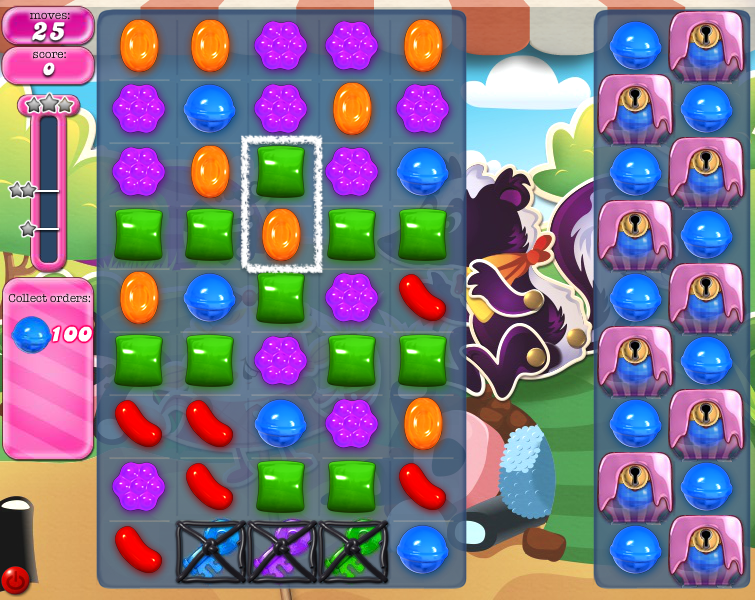
\includegraphics[width=0.4\textwidth]{masters-thesis-master/masters-thesis/contents/02_background/candy_images/Level_1365_Reality.png}
    \label{fig:candy:a}
    }
  \subfloat[]{
    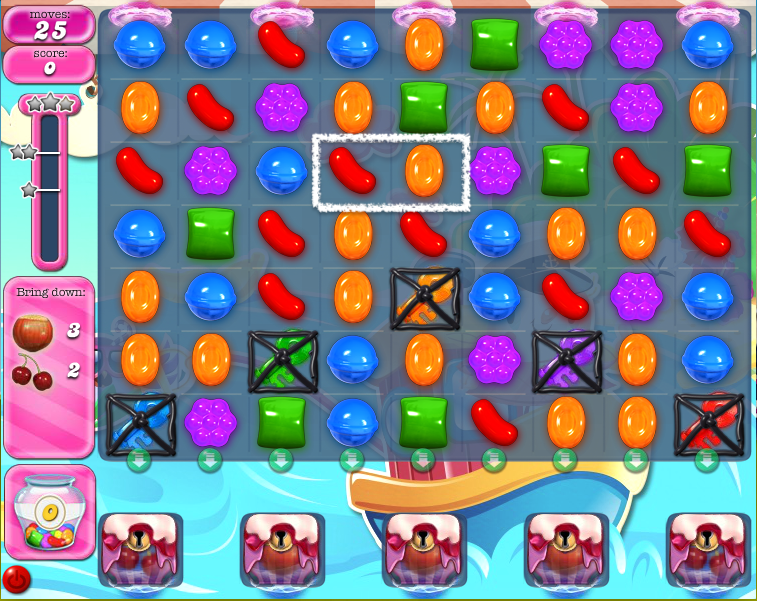
\includegraphics[width=0.4\textwidth]{masters-thesis-master/masters-thesis/contents/02_background/candy_images/Level_1161_Reality.png}
    \label{fig:candy:b}
    }
    
  \subfloat[]{
    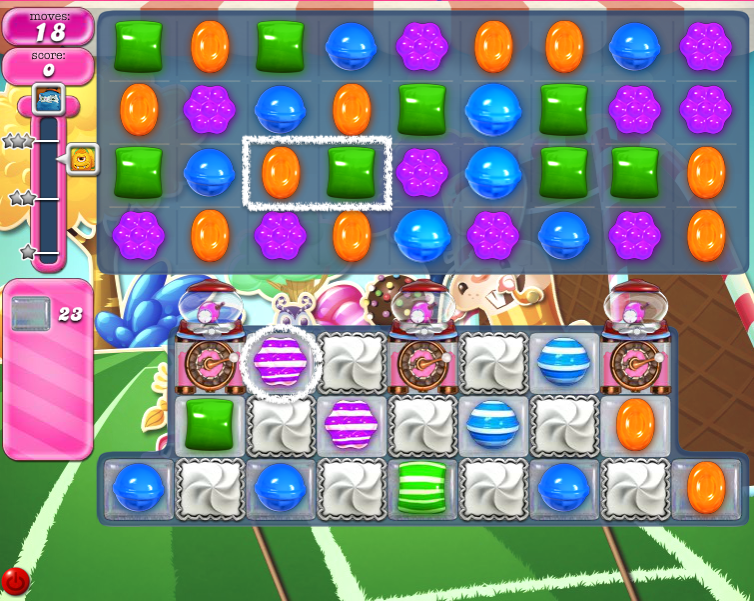
\includegraphics[width=0.4\textwidth]{masters-thesis-master/masters-thesis/contents/02_background/candy_images/Level_1434_Reality.png}
    \label{fig:candy:c}
  }
  \subfloat[]{
    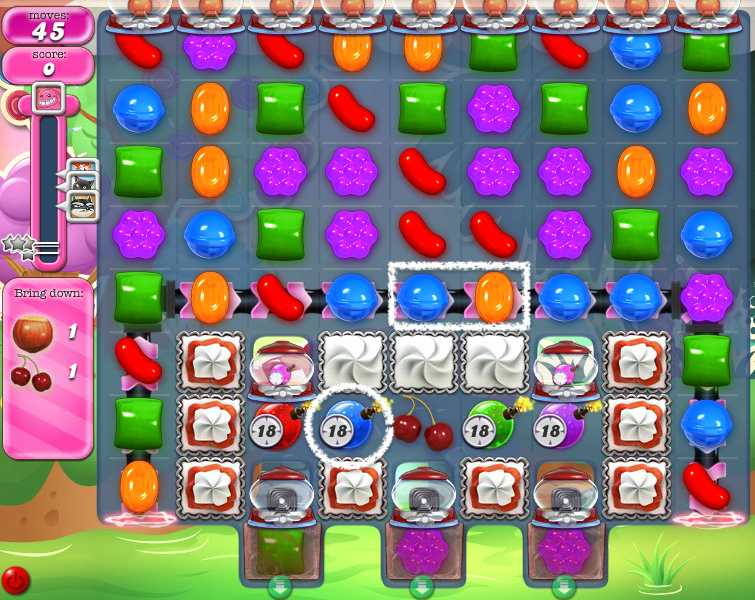
\includegraphics[width=0.4\textwidth]{masters-thesis-master/masters-thesis/contents/02_background/candy_images/Level_963_Reality.png}
    \label{fig:candy:d}
  }
  
    \caption{Examples of legal moves in the game and examples of items. White boxes illustrate examples of possible swaps while white circles illustrate special candies or items.
    }
    \label{fig:candy}
\end{figure}
\noindent
They can be grouped into three main categories:
\begin{enumerate}
    \item \textbf{Pre-level boosters.} Activated before the game starts.
    \item \textbf{In-level boosters.} Activated during the gameplay if the conditions of the game board create any effect when the booster is used. As an example, a player cannot use a "Bomb Cooler" booster if there are no "Bombs" on the game board.
    \item \textbf{Consolation boosters.} Activated at the end of the attempt to prevent failure and retrying.
\end{enumerate}
Some boosters can be used only in specific type of levels. 
In Appendix \ref{boosters} we report a full description of all the boosters with their effects and usage conditions.


\subsection{Gameplay Metrics}
In the last years, game metrics have become popular in the game industry as a source of valuable information about game design. Game metrics are the result of the interaction between the players and the game. Compared to user feedback or surveys, game metrics have the advantage to be objective, not biased by player emotions and they are easier to gather on a large scale. Since our goal is to estimate level difficulty, we use the \acs{sr} on a specific level as a measure of the perceived difficulty. The success rate $sr_{i,k}$ on a level $i$ perceived by a group of players $k$ is defined as follow:
\begin{equation}
 sr_{i,k}= \frac{s_{i,k}}{a_{i,k}} \text{,}
\end{equation}
 \label{eq:sucess_rate}
where $s_{i,k}$ is the sum of the number of successes on level $i$ of each player in group $k$ and $a_{i,k}$ is the sum of the number of attempts on level $i$ of each player in the considered group $k$. The reason why we use the \acs{sr} as a measure of the perceived difficulty is because we believe that if a player needs to try a level many times before solving it, and thus the \acs{sr} is low, he perceives the level as a difficult one, while on the contrary, if a player solves a level in few attempts, he perceives the level as an easy one and the \acs{sr} is high. Another reason why we use the \acs{sr} is to allow a comparison with the state-of-the-art approach. However, since the baseline does not consider different groups of players, we furthermore use a combination of the SR of all the $k$ groups to estimate $sr_{i}$ that is the overall difficulty perceived by all the players on level $i$.

\subsection{Related Work}
Until \textcite{silver_mastering_2016} published their work in 2016, presenting the Google DeepMind’s \textit{AlphaGo} system, most of the research in the game of \textit{Go} was focused on \acs{RL} to teach computer playing the game. The state-of-the-art were \acs{MCTS} programs that simulates thousands of self-play games to estimate the optimal policy. \textcite{silver_mastering_2016} demonstrated how deep neural networks trained on human expert player data can effectively estimate the "value network" used to evaluate board positions and approximate the "policy network" used to select moves in the game of \textit{Go}. The two networks were trained by a combination of reinforcement learning and supervised learning using human expert data. Their research was based on prior work on predicting expert moves in the game of  \textit{Go} using supervised learning techniques \cite{sutskever_mimicking_2008, stern_bayesian_2006, maddison_move_2014}. Their solution is the first computer \textit{Go} program that beat a human professional \textit{Go} player without handicaps. In 2015, \textit{AlphaGo} defeated Fan Hui, a three times European \textit{Go} champion, in all of the 5 matches disputed. In 2016, it beat Lee Sedol, a 9-dan professional player considered one of the best players at \textit{Go}, in a five-game match. 

Similarly to what Silver \textit{et al.} did with \textit{AlphaGo}, \textcite{hlynur_predicting_2017} illustrated how \acs{CNN} can be designed to predict expert moves for the \textit{Othello} game, exceeding the previous state-of-the-art by 5.3\%. He used a \acs{DCNN} trained with handcrafted features and the raw board state as input, showing that removing the handcrafted features decreases the accuracy by only 0.9\% but at the same time allows for a much faster computation. \textcite{chen_game_2017} demonstrated that \acs{CNN} can provide similar performance while requiring fewer resources and training time compared to more complex methods such as deep Q-learning in challenging policy estimation task. More recently, the new Google \textit{AlphaGo Zero} program \cite{silver_mastering_2017} trained solely by self-play reinforcement learning achieved super-human performances, winning 100-0 against the previously published \textit{AlphaGo} system. However, a perfect-play agent that always plays the optimal move and leads to the best possible outcome is out of the scope of this thesis. We aim to model human players and even the best player does not always select the optimal action due to the difficulty of identifing and evaluating each possible move in the \textit{Candy Crush Saga} game. For this reason, it is important that the \acs{AI} agent plays in a human-like manner, making the same sort of errors and therefore using a similar strategy to human players. 

The game of \textit{Go} has several similarities with the game used in our research. First, the grid shape topology of the board and the discrete game action space that make \acs{CNN} a valid approach to simulate gameplay. Second, the vast search space that makes computationally hard to evaluate each possible state-action pair in the game. Third, the observability, since both games have perfect information. Fourth, the time granularity, since both are turn based games and finally, the Markov property, that practically holds for both the games. \textit{Candy Crush Saga} can be considered, for practical purposes, to have the Markov property, even if there are few special cases where specific game items violate this assumption. There is a special candy called "Chameleon candy" that alternates between two colors every turn. However, since this type of candy is really rare in the game, we will treat the game as a Markov process. Even if there are some differences, like the fact that \textit{Go} is a two player zero-sum adversarial game while \textit{Candy Crush Saga} is a single player game or that \textit{Go} is deterministic while \textit{Candy Crush Saga} it is not, we rely on the results of previous work in the game of \textit{Go} to guide our research. Finally, in the last three years, some related work on the \textit{Candy Crush Saga} game has been done. As mentioned in Section \ref{Automatic Playtesting Related Work},  \textcite{poromaa_crushing_2017} used a \acs{MCTS} approach while \textcite{eisen_simulating_2017} and \textcite{purmonen_predicting_2017} used a \acs{CNN}-based approach to simulate gameplay, similarly to what have been done in the \textit{AlphaGo} system.

\section{Theory}

\subsection{Convolutional Neural Networks}
A \acl{CNN} is a specific type of feed-forward artificial neural network that uses a shared-weights architecture and has the translation invariance property. It is mainly used for processing data with a grid-like topology, e.g. time series or images. \acsp{CNN} were inspired by the animal visual cortex where neurons are activated by stimuli from a restricted region of the visual field. A \acs{CNN} consists of an input layer, an output layer and a variable number of hidden layers. Layers can be repeated many times and the output of one layer becomes the input of the next one. An example of a \acs{CNN} architecture is illustrated in Figure \ref{fig:network_architecture_example}.
A key characteristics of \acsp{CNN} is that they have sparse connectivity, meaning that when a convolution operation is performed, the output is determined only by a subset of the input (called receptive field) that depends on the size of the filters. However, in a deep \acs{CNN}, deeper layers may have indirect connections with larger subset of the input. This enable the network to learn complex functions combining simple building blocks. Each hidden layer typically consists of one of the following three types: a convolutional layer, a pooling layer or a fully connected layer. \\

\begin{figure}[t]
    \centering
    
	\begin{tikzpicture}
		\node at (0.5,-1){\begin{tabular}{c}input\end{tabular}};
		
		\draw (0,0) -- (1,0) -- (1,1) -- (0,1) -- (0,0);
		
		\node at (3,3.5){\begin{tabular}{c}   convolutional layer\\   with non-linearities \end{tabular}};
		
		\draw[fill=black,opacity=0.2,draw=black] (2.75,1.25) -- (3.75,1.25) -- (3.75,2.25) -- (2.75,2.25) -- (2.75,1.25);
		\draw[fill=black,opacity=0.2,draw=black] (2.5,1) -- (3.5,1) -- (3.5,2) -- (2.5,2) -- (2.5,1);
		\draw[fill=black,opacity=0.2,draw=black] (2.25,0.75) -- (3.25,0.75) -- (3.25,1.75) -- (2.25,1.75) -- (2.25,0.75);
		\draw[fill=black,opacity=0.2,draw=black] (2,0.5) -- (3,0.5) -- (3,1.5) -- (2,1.5) -- (2,0.5);
		\draw[fill=black,opacity=0.2,draw=black] (1.75,0.25) -- (2.75,0.25) -- (2.75,1.25) -- (1.75,1.25) -- (1.75,0.25);
		\draw[fill=black,opacity=0.2,draw=black] (1.5,0) -- (2.5,0) -- (2.5,1) -- (1.5,1) -- (1.5,0);
		
		\node at (4.2,-1){\begin{tabular}{c}pooling layer \end{tabular}};
		
		\draw[fill=black,opacity=0.2,draw=black] (5,1.25) -- (5.75,1.25) -- (5.75,2) -- (5,2) -- (5,1.25);
		\draw[fill=black,opacity=0.2,draw=black] (4.75,1) -- (5.5,1) -- (5.5,1.75) -- (4.75,1.75) -- (4.75,1);
		\draw[fill=black,opacity=0.2,draw=black] (4.5,0.75) -- (5.25,0.75) -- (5.25,1.5) -- (4.5,1.5) -- (4.5,0.75);
		\draw[fill=black,opacity=0.2,draw=black] (4.25,0.5) -- (5,0.5) -- (5,1.25) -- (4.25,1.25) -- (4.25,0.5);
		\draw[fill=black,opacity=0.2,draw=black] (4,0.25) -- (4.75,0.25) -- (4.75,1) -- (4,1) -- (4,0.25);
		\draw[fill=black,opacity=0.2,draw=black] (3.75,0) -- (4.5,0) -- (4.5,0.75) -- (3.75,0.75) -- (3.75,0);
		
		\node at (8,3.5){\begin{tabular}{c}convolutional layer\\with non-linearities \end{tabular}};
		
		\draw[fill=black,opacity=0.2,draw=black] (7.5,1.75) -- (8.25,1.75) -- (8.25,2.5) -- (7.5,2.5) -- (7.5,1.75);
		\draw[fill=black,opacity=0.2,draw=black] (7.25,1.5) -- (8,1.5) -- (8,2.25) -- (7.25,2.25) -- (7.25,1.5);
		\draw[fill=black,opacity=0.2,draw=black] (7,1.25) -- (7.75,1.25) -- (7.75,2) -- (7,2) -- (7,1.25);
		\draw[fill=black,opacity=0.2,draw=black] (6.75,1) -- (7.5,1) -- (7.5,1.75) -- (6.75,1.75) -- (6.75,1);
		\draw[fill=black,opacity=0.2,draw=black] (6.5,0.75) -- (7.25,0.75) -- (7.25,1.5) -- (6.5,1.5) -- (6.5,0.75);
		\draw[fill=black,opacity=0.2,draw=black] (6.25,0.5) -- (7,0.5) -- (7,1.25) -- (6.25,1.25) -- (6.25,0.5);
		\draw[fill=black,opacity=0.2,draw=black] (6,0.25) -- (6.75,0.25) -- (6.75,1) -- (6,1) -- (6,0.25);
		\draw[fill=black,opacity=0.2,draw=black] (5.75,0) -- (6.5,0) -- (6.5,0.75) -- (5.75,0.75) -- (5.75,0);
		
		\node at (8.5,-1){\begin{tabular}{c}pooling layer \end{tabular}};
		
		\draw[fill=black,opacity=0.2,draw=black] (10,1.75) -- (10.5,1.75) -- (10.5,2.25) -- (10,2.25) -- (10,1.75);
		\draw[fill=black,opacity=0.2,draw=black] (9.75,1.5) -- (10.25,1.5) -- (10.25,2) -- (9.75,2) -- (9.75,1.5);
		\draw[fill=black,opacity=0.2,draw=black] (9.5,1.25) -- (10,1.25) -- (10,1.75) -- (9.5,1.75) -- (9.5,1.25);
		\draw[fill=black,opacity=0.2,draw=black] (9.25,1) -- (9.75,1) -- (9.75,1.5) -- (9.25,1.5) -- (9.25,1);
		\draw[fill=black,opacity=0.2,draw=black] (9,0.75) -- (9.5,0.75) -- (9.5,1.25) -- (9,1.25) -- (9,0.75);
		\draw[fill=black,opacity=0.2,draw=black] (8.75,0.5) -- (9.25,0.5) -- (9.25,1) -- (8.75,1) -- (8.75,0.5);
		\draw[fill=black,opacity=0.2,draw=black] (8.5,0.25) -- (9,0.25) -- (9,0.75) -- (8.5,0.75) -- (8.5,0.25);
		\draw[fill=black,opacity=0.2,draw=black] (8.25,0) -- (8.75,0) -- (8.75,0.5) -- (8.25,0.5) -- (8.25,0);
		
		\node at (12,3.5){\begin{tabular}{c}fully connected layer \end{tabular}};
		
		\draw[fill=black,draw=black,opacity=0.5] (10.5,0) -- (11,0) -- (12.5,1.75) -- (12,1.75) -- (10.5,0);
		
		\node at (13,-1){\begin{tabular}{c}output layer \end{tabular}};
		
		\draw[fill=black,draw=black,opacity=0.5] (12.5,0.5) -- (13,0.5) -- (13.65,1.25) -- (13.15,1.25) -- (12.5,0.5);
	\end{tikzpicture}
	\caption[Architecture of a traditional convolutional neural network.]{Example of CNN architecture. As first introduced by LeCun et al. in 1989, this network alternates between convolutional layers with hyperbolic tangent activation functions to introduce non-linearities and pooling layers. In this representation, the convolutional layers include the activation functions. The grey squares represent the activation maps. The last two layers are fully connected layers. Usually, the output layer uses a softmax activation function. Image generated with code adapted from \cite{stutz_latex-resources:_2018}. }


%    \input{contents/03_method/i00_network_architecture_horizontal}
    \label{fig:network_architecture_example}
\end{figure}
\noindent
\textbf{Convolutional layer:} It applies a convolutional operation to the input and it drastically reduces the number of free parameters allowing to operate with inputs that have high dimensionality like images. Instead of having a connection from each input to each output, as in a fully connected feed-forward neural network, it uses filters (typically of a small size, e.g. 3x3) that are shared between inputs. In this way, each parameter of the filter is used in every position of the input, with various design choices for managing the boundaries. The filters are moved step by step over the input and at each step, the dot product between the filter and the input is computed. The number of units by which the filters shift over the input is the filter stride. On top of that is typically added a non-linear activation function. Each convolutional layer uses one or more filters and each of them, moving over the input, generates an activation map. Finally, all the generated activation maps are stacked together and they constitute the input of the next layer. As a result, the network learns filters that are activated when they detect specific features in the input. Sometimes batch normalization is added at the beginning of the convolutional layer to speed up training and to reduce overfitting. \\ \\
\textbf{Pooling layer:} It reduces the size of each activation map combining multiple outputs of a convolutional layer into a single value. In practice, many types of pooling layers exist and as an example the \textit{max pooling layer} combines multiple output of the previous layer retaining only the maximum value. The idea is to generate smaller representations maintaining only the relevant information introducing invariance to small shifts or distortions. Furthermore, the pooling layer progressively decreases the size of the representation, reducing the number of parameters and the amount of computation required by the network.\\ \\
\textbf{Fully connected layer:} A fully connected layer connects every neuron in the input to every neuron in the output. This type of layer is usually added at the end of the network to feed a \textit{softmax} function and generate a distribution over the output classes. \textcite{lin_network_2013} proposed another strategy called \acf{GAP} to replace the fully connected layers. When using \acs{GAP}, the last convolutional layer has to generate one feature map for each target class. Then, instead of having a fully connected layer, the average of each feature map is computed and the output is fed into a \textit{softmax} function. The advantage of this approach is that since there are no parameters to optimize in the \acs{GAP} layer, overfitting is avoided at this layer. Finally, since from each map only the average value is retained the network is more robust to input spatial translations.\\ \\
The idea of \acs{CNN} \cite{lecun_backpropagation_1989, fukushima_neocognitron:_1980} dates back to the 80s. One of the first applications was to recognize hand-written digits on checks or mails but due to slow computational resources and limited amount of labeled data the research on \acsp{CNN} progressed slowly until 2012. In that year, \textcite{krizhevsky_imagenet_2012} famously developed a network called "AlexNet" and they won, by a large margin, the \acf{ILSVRC} \cite{russakovsky_imagenet_2015}. After this successful result, many variants of \acsp{CNN} have been proposed and new applications have been found. At the time of writing, examples of the most popular and prominent architectures are the inception network and the residual network. The inception network architecture \cite{szegedy_rethinking_2016} was introduced by Google and mainly consists of parallel 1x1, 3x3 and 5x5 convolutional filters combined into several modules. This architecture is able to reduce the number of features, and so the performed operations, compared to the ones of "AlexNet", leading to a very efficient architecture. The main idea of the residual network \cite{he_deep_2016} is to add skip connections allowing the output of a convolutional layer to bypass the next two layers. This approach helps the learning of deep \acsp{CNN} with many layers by better gradient backpropagation. For a deeper understanding about \aclp{NN} and their applications we refer to \cite{goodfellow_deep_2016}.

\subsection{Clustering}

Clustering is an exploratory data mining process that consists of grouping together objects such that elements in the same group (called cluster) are more similar compared to elements in different groups. The term "clustering" refers to the general task and many algorithms to perform it have been proposed. In this thesis we use hierarchical clustering and k-means.

\subsubsection*{Hierarchical clustering}

The algorithm iteratively connects elements to form clusters based on distances between elements. Two main hierarchical clustering approaches exist: the top-down approach starts considering all the elements as a single cluster and iteratively splits them into smaller ones, while the bottom-up approach starts considering all the elements as single clusters and iteratively merges them. Different distance functions can be used, e.g. euclidean distance, hamming distance, cosine distance. Also, the user needs to chose the linkage function, since a cluster consists of multiple data point, the algorithm needs a criterion to select which element to use when computing the distance function. Popular linkage functions are the \textit{single-linkage} function, the \textit{complete-linkage} function and the \textit{average-linkage} function. The \textit{single-linkage} function, considers the minimum of the element distances. As a consequence, the distance $D(X,Y)$ between two clusters $X$ and $Y$ is described by: 
\begin{equation}
 D(X,Y)= \min_{x\in X,y\in Y} d(x,y)  \text{,}
\end{equation}
 \label{eq:single_linkage}
 where $d(x,y)$ denotes the distance between two elements $x$ and $y$. The
\textit{complete-linkage} function considers the maximum of the element distances and it is described by:
\begin{equation}
 D(X,Y)=\max_{x\in X,y\in Y} d(x,y)  \text{,}
\end{equation}
\label{eq:complete_linkage}
instead, the \textit{average-linkage} function, also known as \textit{\acl{UPGMA}} (\acs{UPGMA}), considers the average of the element distances and it is described by:
\begin{equation}\label{eq:average_linkage}
    D(X,Y)=\sum_{x\in X,y\in Y} \frac{d(x,y)}{|X|\cdot|Y|}  \text{,}
\end{equation}
where $|X|$ and $|Y|$ are the cardinalities of clusters $X$ and $Y$ respectively.

Finally, since the general complexity of hierarchical clustering is $\mathcal{O}(n^3)$ this algorithm performs well only for small data sets. However, it does not produce a single partitioning but an extensive hierarchy of merged clusters that can be visualized with a two dimensional diagram known as dendogram \cite{everitt_hierarchical_2011}. Example of a dendogram is illustrated in Figure \ref{fig:dendogram_example}. We can observe how starting with six separate data points the algorithm iteratively merges them until a single cluster containing all the points is obtained.  
\begin{figure}[ht]
    \centering
    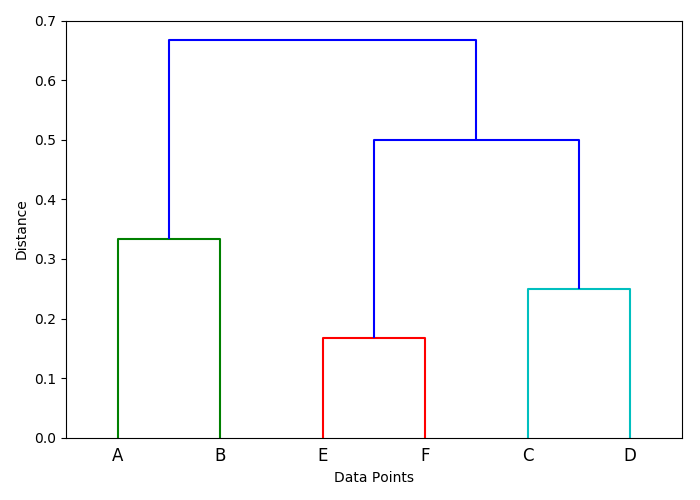
\includegraphics[width=0.6\textwidth]{masters-thesis-master/masters-thesis/contents/02_background/dendogram_example.png}
    \caption{Example of a dendogram. On the x-axis the data points to be clustered, on the y-axis the distance measure. The distance between merged clusters is monotone increasing with the level of the merger. The height of each merge is proportional to the dissimilarity between the data points in each merged cluster. Using a bottom-up approach, the first generated cluster is \{E,F\}, then the second generated cluster is \{C,D\}, the third is \{A,B\} and finally, the last two clusters: \{E,F,C,D\} and the cluster with all the data points \{A,B,E,F,C,D\}.}
    \label{fig:dendogram_example}
\end{figure}

\subsubsection*{K-means}
The algorithm was introduced in 1976 by Stuart Lloyd \cite{lloyd_least_1982}, which is why it is also referred as Lloyd's algorithm, however it was not published outside the Bell labs until 1982 and the term "k-means" was introduced in the same year by James MacQueen. The algorithm aims to partition $n$ observations into $k$  $(\leq n)$ clusters in which each observation belongs to the cluster with the nearest mean. 

\noindent
More formally, given a set of observations $(x_1, x_2, \dots, x_n)$, where each observation is a d-dimensional array, k-means partitions the $n$ observations into $k$ sets $S = {S_1, S_2, \dots, S_k}$ trying to minimize the \acf{WCSS} distances:
\begin{equation}
    \arg\min_{S} \sum_{i=1}^{k} \sum_{x \in S_i} \lVert x - \mu_i \rVert^2 \text{,}
\end{equation}
where $\mu_i$ is the mean of the points in $S_i$.
The most common version of the algorithm uses iterative refinement to assign each observation to a cluster. The number of clusters $k$ is an input parameter of the algorithm and its choice significantly impacts the quality of the output. 
The algorithm, starting with a set of k-means, alternates between two steps until convergence:
\begin{enumerate}
    \item Assignment step: assign each observation to the nearest cluster,
    \item Update step: compute the new means of each cluster, called centroids.
\end{enumerate}
The algorithm converges when no observation changes cluster during the assignment step, however it does not guarantee to find the optimal solution.
A common approach to select the parameter $k$ is the elbow criterion \cite{wierzchon_cluster_2018}. The main idea is to run the algorithm for a range of values of $k$ and computing the \acf{SSE} for each value. Plotting the SSE against the number of clusters $k$, we can chose $k$ by looking at the "elbow" of the line. The idea is to select a small value of $k$ that still has a low SSE. Sometimes this value cannot be unambiguously identified. Regarding the initialization of the centroids, many variants have been proposed and a common approach is to randomly initialize them. For more details about k-means we refer to \cite{wu_advances_2012}.





\chapter{Methods}
\label{chap:method}
 The approach we use for improving automatic playtesting can be divided into three major stages:
 \begin{enumerate}
    \item \textbf{Player modeling.} In this first stage, we model different cohorts of players based on their features. Furthermore, we create artificial agents that simulate their strategies in the game. Since we use human gameplay data to learn the strategies, using the taxonomy defined in \cite{yannakakis_player_2013}, we can classify our method as a direct modeling approach. However, since we do not have any direct strategy feature, we use unsupervised learning techniques in this stage. To model the players we evaluate the following two approaches:
     \begin{enumerate}
        \item \textbf{Clustering players.} First we cluster the players and then we train a different \acs{CNN}-based agent on each player cluster.

        \item \textbf{Clustering simulated strategies.} We train a \acs{CNN}-based agent feeding as input both the player features and the game board. Then, during prediction, by changing the players' input parameters, we can simulate several type of players. Lastly, clustering the simulated strategies we select different agents. 

     \end{enumerate}
    \item \textbf{Gameplay simulation.} On each level, various agents, simulating different player strategies, play the entire level several times. Based on the result of the simulation we compute the \acs{sr} of each agent.
    
    \item \textbf{Players' \acs{sr} prediction.} The final stage is to use the agents' SR on the training levels to fit a prediction model. Using this model we can predict the players' \acs{sr} on new levels.
\end{enumerate}

To perform automatic playtesting, the first stage is executed only one time or when major changes, that made the player models previously defined no longer reliable, are introduced in the game. On the contrary, stages two and three need to be performed each time a new generated game content needs to be tested.

 The novelty of these approaches relies in stage 1. Differently from existing approaches, we model strategies of various cohorts of players by directly learning them from player gameplay data. Some of the existing approaches for automatic playtesting consider only a single strategy while others, even if they simulate various strategies, rely on designers' knowledge or reinforcement learning to model them, without considering player data. Furthermore, to the best of our knowledge, this is the first attempt to use player modeling in a match-three puzzle game. In the next section, we describe the data used in our research. Then, we describe in detail the stages of our two approaches and the evaluation measures.
 
\section{Data}
\subsection{Data Collection}
Since the number of daily active players for the \textit{Candy Crush Saga} game is large and the generated data is greater than what can be used as training data for a \acs{CNN}-based agent in a reasonable amount of time, we decided to track moves and players' statistics only from a subset of all the active players (\textasciitilde1\%). The tracking process of the moves lasted for three months collecting a good and diverse sample of player data. By contrast, the players' statistics, e.g. player's SR or number of boosters used, have been continuously collected while the player was playing the game. This allows to have accurate measures of the player behaviour not only on the levels played during the tracking period.
We collected data from level 1 to level 2945. Levels in the range [1, 2500] are used as training data for the player modeling stage, while levels in the range [2501, 2945] are used as test data in the players' \acs{sr} prediction stage. The split ensures that training data contains all the possible elements of the game since no item is first introduced after level 2500. Furthermore, this split reproduces the same process that is performed in practice where existing levels are used as training data and prediction are performed on future ones. We remind that, as mentioned in Section \ref{delimitations}, we removed levels constrained by time or that contain the "Candy Frog" from the data set. Furthermore, due to an error in the game engine interface that is used by the agents to simulate gameplay in \textit{moves levels}, we removed also this type of levels. Nevertheless, these levels represent only 4.6\% of the total number of levels. This leads to 2161 training levels and 414 test levels.

\subsection{Data Representation}\label{data_representation}
\textbf{Game board features:} Each state is represented by 101 feature layers each one of size 9x9. The feature layers can be categorized into four main types:
\begin{enumerate}
    \item \textbf{Item layers.} There are 80 binary input layers that encode, with a binary representation, the items on the game board. Each of these layers is associated to a single item. Each position in the grid is set to 1 if the item is present and on the contrary, it is set to 0 if the item is not present. Since on each game board, only a subset of all the possible items is present, the layers associated with items that are not on the game board are filled with 0s.
    
    \item \textbf{Objective layers.} There are 19 binary feature layers of this type. Each layer represents a different objective that need to be achieved to win the level. It is filled with 1s if the objective is not yet fulfilled in the given state and contrarily it is filled with 0s if the objective is already fulfilled or if the objective is not requested for the given level.
    
    \item \textbf{Moves left layer.} A layer that represents the number of moves left to finish the level. In the game the maximum number of available moves is 75 and as a consequence the moves left can assume values in the range $\left[1,75\right]$. To give more importance to the last available moves we encode this feature as the ratio of 1 on the number of moves left. Adding this non-linearity has the effect of creating bigger changes in the feature when the moves available are only a few. A change of 1 move left when the available moves are few has a bigger impact on the feature rather than the same change of 1 move when the available moves are a lot. This is because if a player has 75 or 74 available moves he probably do not give too much importance to this difference while if he has only 1 or 2 available moves, the difference becomes important.
    
    \item \textbf{Bias layer.} Additionally, we stack a layer filled with all 1s. This layer allows the network to learn a bias on the position of the performed move in the grid. It is possible that moves in a specific area of the grid are preferred to moves in other positions. For example moves in the lower part of the board could be preferred to moves in the higher part because they increase the probability of creating cascade effects and obtaining more points. This layer can be described as an overall "heatmap" of the performed moves. It add a bias representing the likelihood of choosing a move in a specific position on the grid independently of the content of the game board.
\end{enumerate} 
Note that except for the item layers, the other layers encode only a single value. As a consequence the layers are created by repeating the value in every cell of the 9x9 plane. This allows to exploit the properties of the convolutional neural network also for this input information. \\

\noindent
\textbf{Moves:}
 Each move is a swap between two candies or items. By enumerating the inner edges of the game grid we encode the moves with a scalar number.  As showed in Figure \ref{fig:moves_encoding}, the moves are encoded enumerating first all the horizontal edges and then all the vertical ones. Since the cases where the direction of the move has an impact on the game are rare, we decided to do not distinguish between left-right or right-left moves and between top-down or bottom-up moves. This leads to a total number of 144 possible moves represented with integer values in the range [0, 143]. \\
 \begin{figure}[h!]
    \centering
    \resizebox{0.4
\textwidth}{!}{%
\begin{tikzpicture}[]
\draw[step=1cm,gray,very thin] (0,0) grid (9,9);

\foreach \x in {1,2,3,4,5,6,7,8}{
    \foreach \y [evaluate=\y as \index using int(\x-1+(\y-1)*8)] in {1,2,3,4,5,6,7,8,9}{
        \node at (\x, 9.5 - \y) {\index};
    }
}

\foreach \x in {1,2,3,4,5,6,7,8,9}{
    \foreach \y [evaluate=\y as \index using int(71+\x+(\y-1)*9)] in {1,2,3,4,5,6,7,8}{
        \node at (\x - 0.5, 9-\y) {\index};
    }
}

\end{tikzpicture}
}
    \caption{Moves encoding. Adapted from \cite{eisen_simulating_2017}.}
    \label{fig:moves_encoding}
\end{figure} 

\noindent
\textbf{Player features:}
In Table \ref{tab:player_features} we list all the per-level player features that we use to explore the differences in the player strategies. 
We define as an attempt each trial to solve a level. An attempt is considered ended if the player completes all the objectives, ends all the available moves or decides to exit the level. If a player decides to use a booster that adds extra moves, the attempt ends when also all the extra moves are terminated.  
An attempt is considered ended with a success if the player is able to achieve all the objectives within the constraints of that specific level. Since in this work we do not focus on the subset of levels that have time requirements, the constraint is always a maximum number of moves the player can use to complete the level. As boosters, we consider all the possible types: pre-level, in-level and consolation boosters. Each extra move is considered as a single booster. For example, a plus five extra moves is counted as five boosters. 
\begin{table}[ht]
    \centering
    \small
    \caption{Player features per level}
    \begin{tabular}{l}
    \toprule

    Features \\
    
    \midrule
    % Number of attempts ended \\
    % Number of attempts ended with success \\
    % Number of attempts started \\
    % Maximum number of stars \\
    % Maximum score \\
    % Number of boosters used \\
    Number of attempts ended\\
    Number of attempts ended with success \\
    Number of boosters used \\
    \bottomrule
        
    \end{tabular}
    \label{tab:player_features}
\end{table}

\section{Player Modeling}
The first stage aims to model players with different strategies. The goal of this stage is to generate multiple agents that simulate different strategies instead of having a single model that only simulates an average strategy learnt from all the players. Notice that the strategy learnt by the baseline approach is a combination of examples collected randomly from all the players. As a consequence it only represents an average strategy but it does not represent the strategy of an average player. Since for each player we have the performed moves in different states, a direct comparison between gameplay data cannot tell us how differently the players play. In the following, we describe the two different approaches we introduce for modeling various strategies while learning them directly from player data. 


\subsection{Clustering Players Approach}
The idea is to cluster the players into different groups based on their performance in the game. A first objective with this approach is to discover if players with different performances in the game exhibit a different decision making tendency or strategy and if a \acs{CNN}-based agent is able to capture it, approximating a policy function that shapes their actions in the game. This approach consist of three major stages:
\begin{enumerate}
    \item Computing player metrics
    \item Clustering players
    \item Training of \acs{CNN}-based agents
\end{enumerate}

\paragraph{1. Computing player metrics:}
Using the collected player features, for each player we compute the success rate $sr_i$, on each level $i$, as follows:
\begin{equation}\label{sucess_rate_i}
      sr_i  = \frac{s_i}{a_i} \text{,}
\end{equation}
where $s_i$ is the total number of attempts ended with a success and $a_i$ is the total number of attempts started by the player on level $i$. 
% We decided to use the number of attempt started, to consider as a failed attempts also when a player close the game while he is playing.
Using the per-level SR, we can represent each player with a one dimensional array containing all his SR ordered from level 1 to the last level played by each player. Due to privacy reasons we cannot expose the actual players' SR and as a consequence we use the standardized success rate $\rho_i$ computed as:
\begin{equation}\label{standardized_sr}
       \rho_{i}  = \frac{sr_i - \mu_i }{\sigma_i} \text{,}
\end{equation}
where $\mu_i$ is the average and $\sigma_i$ is the standard deviation of the $SR$ between all the players on level $i$.
An alternative to describe the players, could be to use the maximum number of stars or the maximum score on each level. However, the number of stars can assume only three values while the maximum score contains several outliers. As a consequence, we decided to use the players' SR to more accurately describe the player performances on each level.
Furthermore, in order to have a fair and complete comparison between players, in this approach we restrict our scope only to those players who finished all the training levels. In other words, we eliminate players that did not reach level 2500. This lead to a subset of $32,479$ players. This is also motivated by the fact that we are interested in predicting the perceived difficulty only on new levels and in order to play these levels, a player must have finished all the previous ones. We remind that we tracked only approximately 1\% of the total number of active players.

\paragraph{2. Clustering players:}
Using k-means with euclidean distance we cluster the players' SR distributions to create $k$ clusters of players with similar skill distributions over the training levels. We use k-means since it can work with data with high dimensionality and euclidean distance. Furthermore, k-means computes centroids that can give us a qualitative interpretation of what kind of player group each cluster represents. In order to decide the number of player clusters, represented by the parameter $k$, we use the elbow criterion.

\paragraph{3. Training of \acs{CNN}-based agents:}
Coherently with the defined player clusters, we divide the state-action pair represented by the game boards and the associated performed moves. As a consequence, each cluster data set contains moves tracked from players with similar skill distributions. Then, on each cluster, we train a \acs{CNN} that given the game board as input, predicts the performed move of the player. All the agents are trained for 10 epochs with the same network architecture and the same hyperparameters. For each agent we use 30 million state-action pairs randomly selected from each cluster data set. The test sets consist of 100,000 state-action pairs for each cluster. The training takes about 18 hours on a single machine with 6 CPUs and one Nvidia Tesla K80 GPU. Figure \ref{fig:clustering_players_flow} summarizes the various steps of this approach. 

Finally, as a baseline for this approach, we train an identical \acs{CNN}-based agent with the same amount of data and for the same amount of steps as each cluster agent. The gameplay data are randomly selected from data tracked from player that reached level 2500 without any distinction based on player features. 

\begin{figure}[!ht]
    \centering 
    \resizebox{0.8\textwidth}{!}{%
\begin{tikzpicture}[
decision/.style={diamond, draw, text width=4.5em, text badly centered, node distance=3.5cm, inner sep=0pt},
action/.style   ={rectangle, draw, text width=6em, text centered, rounded corners, minimum height=4em, minimum height=2em},
block/.style   ={rectangle, draw, text width=6em, text centered, rounded corners, minimum height=4em, minimum height=2em},
cloud/.style   ={draw, ellipse, minimum height=2em},
line/.style    ={draw,-latex'},
document/.style = {document, draw, text width=4em, text centered},
node distance=0.5cm, 
auto,]



% Define the nodes
\node[action]                            (dt)        {Tracking data};
\node[action,   right=of dt]             (pp)        {Computing player performance features};
\node[action,   right=of pp]             (cp)        {Clustering players};
\node[action,   right=of cp]             (cd)        {Creating training data sets};
\node[block,    above right=of cd,]      (dpc1)       {Data set from players in cluster 1};
\node[block,     right=of cd,]      (dpc2)       {Data set from players in cluster ... };
\node[block,    below right=of cd,]      (dpc3)       {Data set from players in cluster k};
\node[action,    right= of dpc2]     (tr)        {Training CNNs};
\node[block, above right = of tr]      (nn_1)     {Model trained on cluster 1};
\node[block,  right = of tr]      (nn_2)     {Model trained on cluster ... };
\node[block, below right = of tr]       (nn_3)     {Model trained on cluster k};


% % Connect the nodes
\path[line] (dt) -- (pp);
\path[line] (pp) -- (cp);
\path[line] (cp) -- (cd);
\path[line] (cd) -- (dpc1);
\path[line] (cd) -- (dpc2);
\path[line] (cd) -- (dpc3);
\path[line] (dpc1) -- (tr);
\path[line] (dpc2) -- (tr);
\path[line] (dpc3) -- (tr);
\path[line] (tr) -- (nn_1);
\path[line] (tr) -- (nn_2);
\path[line] (tr) -- (nn_3);



\end{tikzpicture}
}
    \caption{Clustering players flow: We track data from a subset of all the active players. We then compute player performance features and we cluster the players into $k$ clusters. Then, we divide the data set based on the defined clusters. The generated data sets are then used to train $k$ different predictive models.}
    \label{fig:clustering_players_flow}
\end{figure}




\subsection{Clustering Simulated Strategies Approach}
The idea is to let the \acs{CNN} automatically discover the relationship between the player features and the performed moves since the neural network is able to automatically discover even complex relationships between input and output. Similarly to what \textcite{maddison_move_2014} did in their research, we provide the network with additional information regarding the player who performed the move. Compared to the previous approach, where we target one type of player at a time, it has the advantage of avoiding a substantial reduction of training data.
This approach consists of four major stages:

\begin{enumerate}
    \item Computing player metrics
    \item Training the \acs{CNN}-based agent
    \item Predicting moves simulating different players
    \item Clustering the simulated strategies
\end{enumerate}

\paragraph{1. Computing player metrics:}
Since we leave to the \acs{CNN} the task of learning the relationship between player features and predicted moves, this time we use three different dimensions to represent each player. \\
First of all, using the collected player features, we compute the standardized success rate $\rho_{i}$ on each level $i$ as defined in equation \ref{standardized_sr}. Similarly, we computed the average amount of boosters $b_i$, used on each level $i$, as follows:
\begin{equation}
      b_i  = \frac{\text{boosters}_i}{a_i} \text{,}
\end{equation}
where $\text{boosters}_i$ is the total number of boosters used by the player on level $i$ and $a_i$ is the total number of attempts started by the player on level $i$. Subsequently, we compute the standardized value $\beta_i$ as:
\begin{equation}
       \beta_i  = \frac{b_i - \mu_i }{\sigma_i} \text{,}
\end{equation}
where $\mu_i$ is the average and $\sigma_i$ is the standard deviation of the amount of boosters $b_i$ between all the players on level $i$.

Finally, for each player, we compute the following three summary statistics:
\begin{itemize}
    \item The standardized mean success rate $\bar{\rho}$ as:
        \begin{equation}
            \bar{\rho}  = \frac{1}{l} \sum_{i \in L} \rho_i \text{,}
        \end{equation}
    where $L$ is the subset of levels played by the player during the tracking period and $l$ is the number of levels in $L$.
    \item The standardized mean amount of booster $\bar{\beta}$, computed as:
        \begin{equation}
            \bar{\beta} = \frac{1}{l} \sum_{i \in L} \beta_i \text{,}
        \end{equation}
    where $L$ is the subset of levels played by the player during the tracking period and $l$ is the number of levels in $L$.
    \item The number of levels played $l$ during the tracking period.
    % computed as:
    %     \begin{equation}
    %         \lambda  = \frac{l - \mu }{\sigma} \text{,}
    %     \end{equation}
    % where $\mu$ is the average and $\sigma$ is the standard deviation of the number of levels $l$ played between all the players.
\end{itemize}
\noindent
These three player features can be joined together through a unique identifier that represents a specific player. For privacy concern, this unique identifier is anonymised in a way that is not possible to go back to the real player. We decided to use these three metrics because we believe that they can exhaustively represent the various types of players in the investigated game, e.g. skilled vs less skilled players or regular vs occasional players. Since we only take average values between all the levels played by a player, we do not anymore need to restrict our focus to players who completed all the $2,500$ training levels. 

Furthermore, standardizing the \acs{sr}, is not only necessary for privacy reasons but it also helps to take into account that different players may have played different levels. Computing the standard values includes the difficulty of each level in the player metric. However, in order to have meaningful summary statistics, we removed players who played less than 50 levels. This is motivated by the fact that the mean, if computed on few values, becomes too sensitive to outliers. Despite this, we still have tracked data from more than half a million players.


\paragraph{2. Training the \acs{CNN}-based agent:}
We train a \acs{CNN}-based agent that given the game board and the three player features as input, predicts the move performed by the corresponding player. Since players are not divided into groups, we have much more data compared to the previous approach. Therefore, the network is trained for 10 epochs using 125 million state-action pairs as training data. The training data are selected to have approximately 50,000 examples for each level in the range [1, 2500]. As a consequence, each level is represented with a similar amount of data. The training takes about 3 days on a single machine with 6 CPUs and one Nvidia Tesla K80 GPU. The test data consist of 100,000 examples.

\paragraph{3. Predicting moves simulating different players:}
The trained \acs{CNN} acts as a move predictor sensitive to player features. It is able to generate different player moves for the same input game board only by changing the input player parameters. The player features are continuous values and, in theory, we can simulate an infinite number of players. Since our goal is to generate a reasonable amount of different agents, we select for each player features the 5th, 25th, 50th, 75th and 95th percentile and we create an agent for each possible combination of these parameters. These percentiles are selected to have an extensive representation of the real players. We decided to not use the extreme values because they might represent anomalous players. 

Finally, each agent is created by cloning the trained \acs{CNN} and fixing the input player features with a combination among those selected. This generates 125 different agents, each one simulating a different type of player.

\paragraph{4. Clustering the simulated strategies:}
The 125 generated agents can be an exhaustive representation of the different type of players in the \textit{Candy Crush Saga} game. However, simulating gameplay of 125 agents for each level that needs to be tested is computationally expensive. Moreover, some of these agents simulate very similar strategies. In this step, we want to reduce the number of generated agents maintaining only a small number of agents while maximizing the differences in the simulated strategies. To select the agents, we create a validation data set with 10,000 state-action pairs and for each agent we predict the moves. We can then represent each agent with a one-dimensional array containing the predicted moves. Each array can be considered as an explicit representation of the strategy of each agent. Then, we use hierarchical clustering with hamming distance and complete-linkage function on the generated arrays, to group agents with similar strategies. Finally, we select a single agent for each cluster. Figure \ref{fig:clustering_simulated_strategies_flow} summarizes the various steps of this approach. 

As a baseline for this approach, we train a \acs{CNN}-based agent for the same number of steps and using the exact same data but without the input player features. As a result, the baseline agent represents an average policy between all the players and simulates a single strategy. It is worth to remember that the objective of this thesis is not to directly compare the two experimented approaches, but to understand if each approach is better than its own baseline answering if player modeling can improve automatic playtesting.
 

\begin{figure}[ht!]
    \centering
    \resizebox{0.8\textwidth}{!}{%
\begin{tikzpicture}[
decision/.style={diamond, draw, text width=4.5em, text badly centered, node distance=3.5cm, inner sep=0pt},
action/.style   ={rectangle, draw, text width=6em, text centered, rounded corners, minimum height=4em, minimum height=2em},
block/.style   ={rectangle, draw, text width=6em, text centered, rounded corners, minimum height=4em, minimum height=2em},
cloud/.style   ={draw, ellipse, minimum height=2em},
line/.style    ={draw,-latex'},
document/.style = {document, draw, text width=4em, text centered},
node distance=0.5cm, 
auto,]



% Define the nodes
\node[action]                            (dt)        {Tracking data};
\node[action,   right=of dt]             (pf)        {Computing player features};
\node[action,   right=of pf]             (tr)        {Training CNN};
\node[action,   right=of tr]             (sf)        {Selecting player features};
\node[block,    above right=of sf,]      (ag1)       {Agent 1};
\node[block,     right=of sf,]      (ag2)       {Agent ... };
\node[block,    below right=of sf,]      (ag3)       {Agent 125};
\node[action,    right= of ag2]     (pr)        {Predict moves on validation set};
\node[action,    right= of pr]     (css)        {Clustering simulated strategies};
\node[block, above right = of css]      (nn_1)     {Model 1};
\node[block,  right = of css]      (nn_2)     {Model ... };
\node[block, below right = of css]       (nn_3)     {Model k};


% % Connect the nodes
\path[line] (dt) -- (pf);
\path[line] (pf) -- (tr);
\path[line] (tr) -- (sf);
\path[line] (sf) -- (ag1);
\path[line] (sf) -- (ag2);
\path[line] (sf) -- (ag3);
\path[line] (ag1) -- (pr);
\path[line] (ag2) -- (pr);
\path[line] (ag3) -- (pr);
\path[line] (pr) -- (css);
\path[line] (css) -- (nn_1);
\path[line] (css) -- (nn_2);
\path[line] (css) -- (nn_3);



\end{tikzpicture}
}
    \caption{Clustering simulated strategies flow: We track data from a subset of all the active players. We then compute player features and we train a \acs{CNN}-based agent giving as input the game board and the player features. Then, we predict moves on a validation set with different agents. Each agent shares the same network but it has a different player input feature combination. Finally, we cluster the simulated strategies and we select the agents maximizing the differences in their predictions.}
    \label{fig:clustering_simulated_strategies_flow}
\end{figure}


\section{Gameplay Simulation}
\textcite{eisen_simulating_2017} illustrated how a \acs{CNN}-based agent can be used to predict human moves in the \textit{Candy Crush Saga} game. Since his approach reached the best performance to date, we decided to use a similar network architecture for predicting player moves. 

\subsection{Player Moves Prediction}
%After the successful results in predicting expert moves in the game of \textit{Go} \cite{silver_mastering_2017}, 
This stage is identical for both the experimented approaches since it does not depend on how we created the various agents. To simulate gameplay, for each agent, we use the following infrastructure. Several machines run the game engine, integrated with the agent interface, that takes care of simulating the attempts. At the same time, on a web server we run various replicas of the \acsp{CNN}. We decided to separate these two components to allow the agent to use different approaches to select the moves, abstracting it from the predictions of the neural network. The agent interfaces communicate with the \acsp{CNN} trough a component called load balancer. The main task of the load balancer is to redirect the requests received from the agent interfaces to the \acs{CNN} with the lowest utilization. The requests contain the encoded game state obtained from the agent. The response is the predicted probability distribution over the 144 possible moves. When an attempt is finished, the results of the simulation are saved on a table using MySQL database.

For each agent we ran a simulation on both training and test levels. A simulation consists of 100 attempts on each level. This number is selected to run the simulation in a reasonable amount of time. Each attempt runs with a different seed that causes the game to generate different random content. However, to have a fair comparison between agents, the selected seeds are the same for each simulation. The simulation takes approximately 18 hours for each agent while running on a total of 26 \acf{vCPU} cores and 24 GB of memory. The \acs{vCPU} cores are divided between the various components as follow: 18 \acs{vCPU} cores are used to run the bot interface, 2 \acs{vCPU} cores are used by the load balancer while the remaining 6 \acs{vCPU} cores are used to run the \acsp{CNN}. This allocation of resources has demonstrated to work well in practice, in term of speed and utilization. All the computational resources are allocated using a cloud service provider.
When the network is used as an agent to simulate gameplay, a greedy policy is used to select the moves. Since the output of the network is a probability distribution over the 144 available moves, the greedy policy selects the move with the highest predicted probability. 
% Only in the unusual case in which the greedy move is not a legal one, in order to progress in the gameplay simulation, we select the legal move with the highest predicted probability. 
Finally, from the results of the simulations we compute the agents' \acs{sr} on each level. These metrics indicate how difficult a level is for each agent.


\subsection{Convolutional Neural Network Architecture}
When designing a \ac{CNN}, several architectural choices need to be taken and various hyperparameters need to be selected. In this research we rely on the choices made and discussed in \cite{eisen_simulating_2017} with only small changes to the input layer to consider the player features in the clustering simulated strategies approach. For completeness, in this section, we describe the network architecture used for predicting the moves given the states. The network, illustrated in Figure \ref{fig:network_architecture}, is trained with Adam optimizer \cite{kingma_adam:_2014} and an initial learning rate of 0.0005.

\paragraph{Input Layer:}
The input of the network slightly differs between the two approaches we illustrate in our research. In the clustering players approach, the input is represented by 101 layers each one of size 9x9 to represent a game board as described in Section \ref{data_representation}. To train the network we use mini-batch gradient descent with a batch size of 2048 examples since it showed to be a good compromise between accuracy and efficiency. This lead to an input of size [2048x9x9x101]. Differently, in the clustering simulated strategy approach, we add three player features as input leading to an input size of [2048x9x9x104].

\paragraph{Convolutional Layers:}
The network consists of 11 convolutional layers with 35 filters per layer and kernel size of 3x3. Since we do not want the translation invariance property of \acs{CNN} architectures because we want to accurately determine which move to select, we do not use pooling layers. Furthermore, since the game board is only 9x9, we want the output size to be the same as the input size. As a consequence, we used zero-padding and filters with stride of 1.
Subsequently, a last convolutional layer with 144 filters is added to the network. The range $\left[0,143\right]$ represents the encoding of the 144 possible moves that the network can predict.
Each convolutional layer is followed by an \acf{ELU} activation function. The \acs{ELU} function, introduced by \textcite{clevert_fast_2015}, is computed as follow:
\begin{equation}
    f(x)= 
            \begin{cases}
                x,                 & \text{if } x > 0\\
                \alpha (e^x-1),     & \text{if } x \leq 0  
            \end{cases}
\end{equation}
where the \acs{ELU} hyperparameter $\alpha$ controls the saturation of the \acs{ELU} function for negative values. As suggested in \cite{clevert_fast_2015}, we use a value of $\alpha=1.0$. Compared to \acf{ReLU} function, the \acs{ELU} function has also negative values, which allow the network to push the mean of each activation map closer to zero, reducing the \textit{bias shift} typical of \acs{ReLU} functions. Furthermore, as showed in \cite{eisen_simulating_2017}, the \acs{ELU} improved the accuracy of the model by 2.5\% compared to the \acs{ReLU} function.  

\paragraph{Output Layer:}
The output layer is a \acs{GAP} layer that transforms the 144 activation maps of the last convolutional layers into 144 scalars retaining only the average value for each map. Using a \acs{GAP} layer also motivates the choice of encoding the information represented by scalar values into feature planes by replicating the number on all the cells of the 9x9 grid. Otherwise a fully connected layer would be necessary to include these features into the model. Finally, in order to have a probability distribution over the predicted moves, the \textit{softmax} function is applied.

\begin{figure}
    \centering
    \resizebox{\textwidth}{!}{%
\begin{tikzpicture}[
decision/.style={diamond, draw, text width=4.5em, text badly centered, node distance=5cm, inner sep=0pt},
action/.style   ={rectangle, draw, text width=6em, text centered, rounded corners, minimum height=4em, minimum height=2em},
block/.style   ={rectangle, draw, text width=7em, text centered,minimum height=2em, node distance=1cm,},
cloud/.style   ={draw, ellipse, minimum height=2em},
scalar_op/.style   ={text width=6em, text centered, minimum height=2em, node distance=1cm,},
half_scalar_op/.style   ={text width=1em, text centered, minimum height=2em, node distance=0.5cm,},
line/.style    ={draw,-latex'},
document/.style = {document, draw, text width=4em, text centered},
node distance=0.5cm, 
auto,]% Define the nodes
\node [scalar_op] (i) {input};
\node[block, right=of i, ] (c1) {3x3 conv,\\35 filters,\\ELU activation};
\node[below=of c1, shift={(0,5mm)}]{x11};
\node[block, right=of c1, ] (c12) {3x3 conv,\\144 filters,\\ELU activation};
\node[block, right=of c12, ](avg){global average pooling};
\node[block, right=of avg](sm){softmax};
\node[scalar_op, right=of sm](out){output};
%
%\draw[decorate,decoration={mirror,brace,amplitude=5pt,raise=50pt},yshift=10pt,yshift=0pt,-]
%  ([yshift=.5cm]c1.center) -- ([yshift=-.5cm]c11.center) node[black,midway,xshift=-70pt,rotate=90] (convlayers) {11 conv layers zero-padding to maintain dimensions};

%
%% Connect the nodes
\path (i) edge [->] (c1)
(c1) edge [->] node {} (c12)
(c12) edge [->] node {} (avg)
(avg) edge [->] (sm)% 
(sm) edge [->] (out);% 

%% draw cubes 
\pic at ([yshift=3cm]i.center) {annotated cuboid={width=9, height=9, depth=101, scale=.04, units=}}(a);
% 
\pic at ([yshift=3cm, xshift=0.5cm]c1.center) {annotated cuboid={width=9, height=9, depth=35, scale=.04, units=}}(b);
% \pic at ([xshift=3cm]inter.center) {annotated cuboid={width=9, height=9, depth=35, scale=.04, units=}}(c);
%%  \pic at ([xshift=3cm]c11.center) {annotated cuboid={width=9, height=9, depth=35, scale=.04, units=}}(c);
%
% 
\pic at ([yshift=3cm, yshift=-.5cm]c12.center) {annotated cuboid={width=9, height=9, depth=144, scale=.04, units=}};


%
%% draw vectors 
%\path ([xshift=2.5cm]l.center) edge [below,|-|] node {144} ([xshift=6cm]l.center);
%
\path ([xshift=-0.5cm,yshift=1.7cm]avg.center) edge [below,|-|] node[shift={(3mm,0)}] {144} ([yshift=4.2cm, xshift=1.8cm]avg.center);
\path ([xshift=-0.5cm,yshift=1.7cm]sm.center) edge [below,|-|] node[shift={(5mm,0)}] {144} ([yshift=4.2cm, xshift=1.8cm]sm.center);
\path ([xshift=-0.5cm,yshift=1.7cm]out.center) edge [below,|-|] node[shift={(5mm,0)}] {144} ([yshift=4.2cm, xshift=1.8cm]out.center);

 
% % Connect the cubes with arrows
% \path ([xshift=3cm, yshift=-1cm]i.center) edge [right,->] ([xshift=3cm, yshift=1cm]c11.center);

% \path ([xshift=3cm, yshift=-1cm]c11.center) edge [right,->] ([xshift=3cm,yshift=.2]c12.center);

% \path ([xshift=3cm, yshift=-1.5cm]c12.center) edge [right,->] ([xshift=3cm,yshift=-13]avg.center);

% \path ([xshift=3cm,]l.center) edge [right,->] ([xshift=3cm,yshift=0.2cm]sm.center);

\end{tikzpicture}
}
%    \input{contents/03_method/i00_network_architecture_horizontal}
    \caption{Convolutional neural network architecture used in the clustering players approach, with data representations for each layer. In the clustering simulated strategies approach, the input layer changes from 101 to 104 input features. Image generated with code adapted from \cite{eisen_simulating_2017}.} 
    \label{fig:network_architecture}
\end{figure}


\section{Players' SR Prediction}
At this step we have the per-level agents' \acs{sr} on both training and test levels. As demonstrated in \cite{eisen_simulating_2017}, the agents' \acs{sr} does not directly map to the \acs{sr} of the players. However, they are correlated. In this stage we combine the agents' \acs{sr} on test levels to better predict the players' \acs{sr} compared to the baseline in each of the two approaches. In order to not expose the actual values of the players' \acs{sr} for privacy reasons, we scaled the players' \acs{sr} dividing each value by the difference between the maximum and the minimum \acs{sr}.
As a consequence, the scaled players' success rate $sr_i^\prime$ on level $i$ is defined as:
\begin{equation}\label{eq:scaled_sr}
    sr_i^\prime = \frac{sr_i}{max(sr_i) - min(sr_i)} \text{,}
\end{equation}
where $sr_i$ is the actual players' success rate on level $i$, $max(sr_i)$ is the maximum success rate and $min(sr_i)$ is the minimum success rate between all the levels. This has the effect of scaling the values while maintaining the same distribution.
Furthermore, since the distributions of \acs{sr} for both the players and the agents have a positive skew, meaning that the mass of the distribution is concentrated on the left, we apply a log transformation on each variable. Nevertheless, applying the log transformation causes the values of the \acs{sr} that were zero to become minus infinite. As a consequence, we decided to use the mean value to predict the players' \acs{sr} when the agent's \acs{sr} is zero. An alternative could be to use the $log(x + 1)$ transformation where in our case $x$ is the agent's \acs{sr}. However, we prefer to handle the levels where the agent failed in a different way because when the agent's \acs{sr} is zero does not necessary mean that the level is extremely difficult. This is also motivated by the fact that for extremely low values of the agents' \acs{sr} there is no linear relationship with the players' \acs{sr}. Since levels are designed and tested to be solvable by humans within a reasonable number of attempts, extremely low values of the players' \acs{sr} do not exist. This explains why there is no linear relationship between extremely low values of the log of the players' and the log of the agents' \acs{sr}. We excluded those levels where all the agents and the baseline failed since they would just introduce noise to the comparison of the approaches. Finally, we decided to not use a cross-validation approach for two reasons: first, because we want to produce the same scenario that would be used in practice where the existing levels are used to make predictions on new levels and second because we trained the agents on the training levels only and we let them play on new ones to reduce overfitting. 
In this stage we use two slightly different methods for the two experimented approaches. 

\subsection{Clustering Players Approach}
Using the players' and agents' \acs{sr} on training levels we fit a linear regression model for each agent, including the baseline. Then, we use the linear models to predict the players' \acs{sr} on the test levels. 
An issue we need to take into account is that in \textit{Candy Crush Saga}, levels might have been modified during time. Since the players' \acs{sr} is computed from the players' attempts at the time they have played while the agents simulate the current version of the levels, we eliminate from our data set those levels that have drastically changed. We classify a modified level as drastically changed if the players' \acs{sr} on it changes more than $50\%$. These levels represent 18\% of the total number of levels and removing them leads to 1722 training levels and 388 test levels. 

Each model predicts the players' \acs{sr} of the specific group $k$ that it represents. In order to compare our approach with the state-of-the-art, we combine the predictions of the agents on each test level $i$, computing the overall predicted success rate $\widehat{sr}_i$ between all the players using a weighted average as follow:
\begin{equation}\label{combination}
    \widehat{sr}_i = \sum_{j = 1}^{k} w_j \cdot \widehat{sr}_{i,j}  \text{,}
\end{equation}
where $k$ is the number of defined agents, $w_j$ is the percentage of players in cluster $j$ and $\widehat{sr}_{i,j}$ is the success rate on level $i$ of the agent trained with data from cluster $j$.
The idea is that the predictions of each agents have a weight that depends on the percentage of players that the agent simulates.
Finally, the predictions of this model are compared to the predictions of the linear regression model created from the baseline agent's \acs{sr}.

\subsection{Clustering Simulated Strategies Approach}

Since we cannot precisely determine how many players each agent represents, in this approach we predict on each test level $i$, the overall predicted success rate $\widehat{sr}_i$ between all the players using a single linear regression model. The model takes as input all the $k$ agents' success rates $\widehat{sr}_{i,j}$. The predictions of this model are then compared to the predictions of a linear regression model trained with the baseline agent's \acs{sr}. 


\section{Evaluation Metrics}

In this section we describe the metrics we use to evaluate both the move prediction performance of the \acs{CNN} models as well as the \acs{sr} estimation performance of the linear regression models.

\subsection{Player Moves Predictions}
To evaluate the performances of the \acs{CNN}-based agents in predicting player moves we use the top-1 and top-3 prediction accuracy. The top-1 and top-3 prediction accuracy are the ratios of correct predictions to the total number of predicted actions. However, the top-1 accuracy considers a prediction as correct if the correct move coincides with the predicted one while the top-3 accuracy considers a prediction as correct if the right move appears in the top three predicted ones.

\subsection{Linear Regression Models}
To compare the baseline agent with our approach, we compute three different measures. The goal is to see how close the predictions of each approach are to the actual observed values compared to the baseline. The measures used in this research are: the \acf{MAE}, the \acf{MSE} and the adjusted R-squared ($\text{R}^2_{adj}$).
The \acs{MAE} describes the means of the absolute differences between the predicted and the observed players' \acs{sr} on all the $n$ test levels and it is defined as:
\begin{equation}
    \text{MAE} = \frac{1}{n} \sum_{i=1}^{n} |\widehat{sr}_i - {sr}_i| 
\end{equation}
The \acs{MSE} measures the mean of the squared differences between the predicted and the observed players' \acs{sr} on all the $n$ test levels and it is described as:
\begin{equation}
    \text{MSE} = \frac{1}{n} \sum_{i=1}^{n} (\widehat{sr}_i - {sr}_i)^2
\end{equation}
The \acs{MSE} has the property of strongly penalizing large deviations from the observed values.
Finally, the adjusted R-squared, explains the predictive power of the regression models considering the number of predictors. It decreases when a predictor improves the model less than what would be improved by chance. This is a desirable property since in the clustering simulated strategies approach, we compare a method that uses multiple predictors with the baseline approach that only uses a single predictor. The adjusted R-squared is defined as:
\begin{equation}
    \text{R}^2_{adj} = 1 - [\frac{(1-R^2)(n-1)}{n-k-1}] \text{,}
\end{equation}
where $n$ is the number of data points, $k$ is the number of predictors excluding the constant and $\text{R}^2$ equals the square of the Pearson correlation coefficient \cite{benesty_pearson_2009} between the observed and the predicted values.

\chapter{Results}
\label{chap:results}
% \section{Preliminary Data Analysis}

\section{Player Modeling}
We illustrate in this section the results of the two experimented approaches regarding the modeling of the players and the creation of the various agents that simulate different strategies.

\subsection{Clustering Players Approach}
We represented each player with a one dimensional array containing all his $2,500$ standardized success rates $\rho_i$ on the training levels. However, some players have missing SR for various reasons. The missing data points represent $5.16\%$ of the total number of players' \acs{sr}. In order to have comparable players' \acs{sr} distributions, we reconstructed the missing values using linear interpolation.
Figure \ref{fig:player_distribution} shows two examples of standardized players' SR distributions over the training levels.

\begin{figure}[h]
  \centering
  \subfloat[]{
    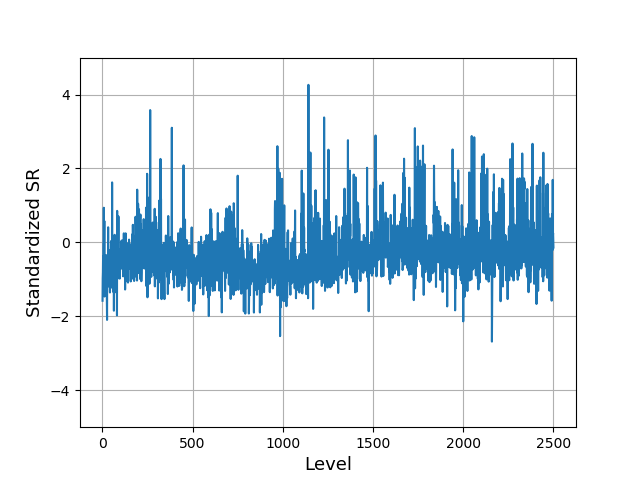
\includegraphics[width=0.45\textwidth]{masters-thesis-master/masters-thesis/contents/04_results/clustering_players_images/one_player_sr_distribution.png}
    \label{fig:player_distribution:a}
    }
  \subfloat[]{
    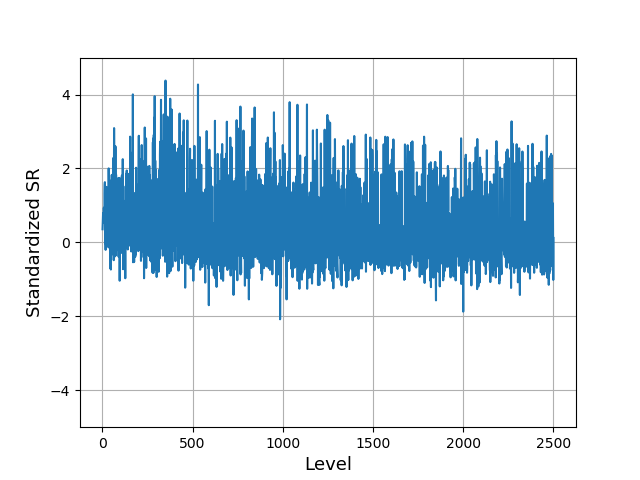
\includegraphics[width=0.45\textwidth]{masters-thesis-master/masters-thesis/contents/04_results/clustering_players_images/one_player_sr_distribution_2.png}
    \label{fig:player_distribution:b}
    }
    \caption{Two examples of standardized players' SR distributions over the levels in range [1, 2500]. 
    }
    \label{fig:player_distribution}
\end{figure}
\noindent
In order to select the number of player clusters $k$, we used the elbow criterion. By looking at the plot of the SSE against several numbers of $k$, as illustrated in Figure \ref{fig:select_k}, we decided to group the players into six different clusters. 
\begin{figure}[h]
  \centering
    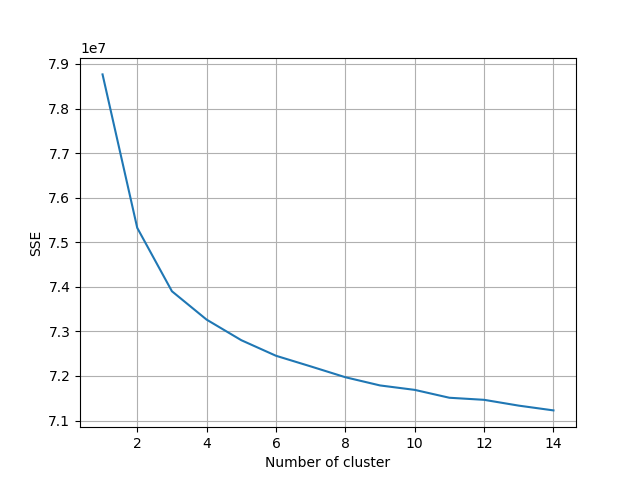
\includegraphics[width=0.6\textwidth]{masters-thesis-master/masters-thesis/contents/04_results/clustering_players_images/select_k.png}
    \caption{Elbow line used to select the number of clusters $k$. On the x-axis various numbers of $k$ while on the y-axis the SSE of the corresponding generated clusters. The plot shows that reasonable values of $k$ are between 3 and 8.}
    \label{fig:select_k}
\end{figure}
Subsequently, we applied k-means to the players' SR distributions. Figure \ref{fig:k_means} shows the centroids of the generated clusters. By looking at the centroids, we can qualitatively describe the six different types of players represented by each cluster. Players in cluster 1 (orange) show a consistently high standardized SR and the cluster can therefore represents very good players. On the contrary, players in cluster 4 (purple), show a very low standardized SR distribution and the cluster can therefore represents less skilled players. 
Players in cluster 0 (blue) show a decreasing standardized SR and the cluster can therefore represents players that encounter difficulties in progressing the game. On the contrary, players in cluster 3 (red), show an increasing standardized SR and the cluster can therefore represents players that learn good strategies over time. Finally, players in cluster 2 (green) show a standardized SR distribution close to the average as well as players in cluster 5 (brown), but with slightly less variance over the levels.
\begin{figure}[h]
  \centering
    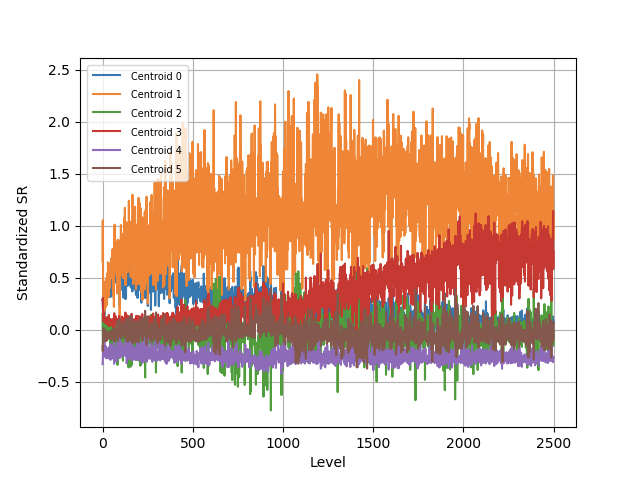
\includegraphics[width=0.6\textwidth]{masters-thesis-master/masters-thesis/contents/04_results/clustering_players_images/centroids_6_clusters.png}
    \caption{Centroids of the 6 generated clusters. The x-axis represents the training levels while on the y-axis the standardized SR. Centroid 0, in blue, represents players with decreasing standardized SR, centroid 1, in orange, represents players with high standardized SR, centroid 2, in green, represents players with average standardized SR, centroid 3, in red, represents players with increasing standardized SR, centroid 4, in purple, represents players with low standardized SR and finally, centroid 5, in brown, represents players with average standardized SR but with less variance compared to centroid 3. [This image is better viewed in color].
    }
    \label{fig:k_means}
\end{figure}
Since k-means generates clusters with different sizes, in Table \ref{tab:clusters_features} we reported the number of players in each cluster. Note that cluster 1 contains only 2\% of the players, indicating the possibility that these players are simply outliers. To understand if the variability in the standardized players' SR distribution has an impact on the obtained clusters, we tried to cluster the levels into few buckets based on their difficulty and then represent each player with his average standardized SR distribution over the buckets. Since we obtained similar player clusters we decided to use the simplest approach avoiding to introduce a second clustering step on the levels.


\begin{table}[h]
    \centering
    \small
    \caption{Player clusters}
    \begin{tabular}{c l c S}
    \toprule
    Cluster \# & Color & \text{\# of Players} & \text{\% of Players} \\
    \midrule
    0 & blue & 3460 & 10.65  \\
    1 & orange & 652 & 2.00 \\
    2 & green & 7042 & 21.68  \\
    3 & red & 2581 & 7.95 \\
    4 & purple & 8958 & 27.58  \\
    5 & brown & 9786 & 30.13 \\
    \bottomrule
    \end{tabular}
    \label{tab:clusters_features}
\end{table}

\subsection{Clustering Simulated Strategies Approach}

In this approach we decided to add other two player features: the standardized mean amount of booster $\bar{\beta}$ and the number of levels played $l$ during the tracking period. Furthermore, instead of using the distribution of the \acs{sr} along the levels, we aggregated the values to have a single measure $\bar{\rho}$, that represents the overall skill of the player. Then, we let the network detect the relationship between these features and the performed move. After training the \acs{CNN}, we predicted on a validation set of 10,000 states with 125 different input player feature combinations. We generated all the possible combinations using the 5th, 25th, 50th, 75th and 95th percentiles of each player feature. The moves predicted by each agent are then considered as a sort of explicit representation of the simulated strategy of the agent. Clustering the simulated strategies we selected six agents that maximized the difference in the predicted moves. Results showed that the 25th and the 75th percentiles were never used by any of the obtained agents. This is reasonable since the player features are real numbers and extreme values lead to more diverse strategies. As a consequence we experimented repeating the clustering only with the 5th, 50th, and 95th percentiles of each player feature. Figure \ref{fig:hierarchical_clustering} shows the dendogram generated by hierarchical clustering. It shows that most of the agents have very similar predictions, however the six most different agents have a difference in the simulated strategies of at least 13\%. This means that by changing the player features the network predicts differently. Table \ref{tab:agents_generated_sim_strategies} shows the selected agents, their player features and a possible interpretation of the simulated types of players. The selected agents are the ones that on each of the six major clusters have a distance to their merged cluster that is the maximum compared to the other agents in the same cluster. As distance measure we used the hamming distance between the simulated strategies. The hamming distance represents the percentage of moves that the compared agents predict differently. We can observe that the two most diverse agents select different moves 31\% of the time.
\begin{figure}[h]
  \centering
    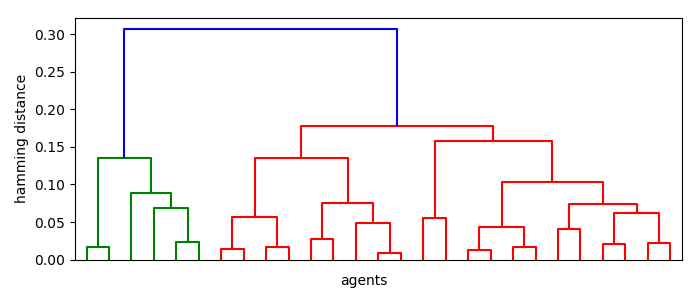
\includegraphics[width=0.6\textwidth]{masters-thesis-master/masters-thesis/contents/04_results/Player_Modeling/Sim_strategies/Plots/hierarchical.png}
    \caption{Dendogram illustrating the differences in the simulated strategies of 27 different agents. The x-axis represents the 27 different generated agents with different combinations of the standardized mean success rate $\bar{\rho}$, the standardized mean amount of boosters $\bar{\beta}$ and the number of different levels played $l$. The y-axis represents the percentage of moves that the agents predict differently. 
    }
    % Each agent share the same network but uses different player features as input. The player features on the x-axis are abbreviated as follows: "bo" means the standardized mean amount of boosters $\bar{\beta}$, "di" means the standardized number of different levels played $l$ while "sk" means skill and represent the standardized mean success rate $\bar{\rho}$.
    \label{fig:hierarchical_clustering}
\end{figure}
\begin{table}[h]
    \centering
    \small
    \caption{Agents generated by clustering simulated strategies} 
       \begin{tabular}{l S c S l }
    \toprule
    
    Agent & \text{Skill ($\bar{\rho}$)} &  Levels played ($l$) & \text{Boosters ($\bar{\beta}$)} & Description \\

    \midrule
    Agent 0 & -0.76  & 241 & -0.06   & less skilled player \\ 
    Agent 1 & -0.76  & 69  & 1.51    & less skilled occasional booster player \\ 
    Agent 2 & 0.96   & 927 & -0.37   & skilled regular non-booster player \\ 
    Agent 3 & 0.96   & 927 & 1.51    & skilled regular booster player \\ 
    Agent 4 & 0.05   & 241 & 1.51    & booster player \\ 
    Agent 5 & 0.96   & 69  & -0.37   & skilled occasional non-booster player \\ 
    
    \bottomrule
    \end{tabular}
    \label{tab:agents_generated_sim_strategies}
\end{table} 


\section{CNNs Training and Prediction}

Except for the input size, we used the same network architecture for the two experimented approaches. Regarding the clustering players approach, Table \ref{tab:Top1_training_test_accuracy} reports the top-1 accuracy, while Table \ref{tab:Top3_training_test_accuracy} reports the top-3 accuracy of each agent. 
With bold we indicate the agent with the best accuracy on each data set. Each row represents a different data set. The first row represents the training accuracy of each agent on its own last mini-batch (consisting of 2048 examples). The remaining rows represent the test accuracy on different test data sets (each one consisting of 100,000 examples). By looking at the accuracy on the test data sets, we observed that in both the top-1 and top-3 accuracy, each agent better represents the players in its cluster compared to the baseline approach. This indicates that the \acs{CNN} model is able to learn different policies by changing the input data used during training. However, we observed that there is only a small difference between the prediction accuracy of the agents and the baseline. This is explained by the fact that we ran experiments with thousands of different players. As a consequence, even if we divide the data, each cluster contains examples from many different players and the \acs{CNN} learns the average strategy of the players on each cluster. Combining data of such a large number of players reduces the differences in the strategies learnt.
\begin{table}[H]
    \centering
    \small
    \caption{Clustering players. Top-1 training and test accuracy} 
    
    \begin{tabular}{l c c c c c c c}
    \toprule

    Data set & Agent 0 & Agent 1 & Agent 2 & Agent 3 & Agent 4 & Agent 5 & Baseline \\
    
    \midrule
    Training data & \textbf{52.97} & 47.46 & 48.77 & 46.39 & 49.10 & 51.78 & 49.74\\
    \hline
    Test cluster 0 data & \textbf{51.93} & - & - & - & - & - & 51.16 \\
    Test cluster 1 data & - & \textbf{47.06} & - & - & - & - & 46.02\\
    Test cluster 2 data & - & - & \textbf{53.03} & - & - & - & 51.97\\
    Test cluster 3 data & - & - & - & \textbf{46.78} & - & - & 45.54\\
    Test cluster 4 data & - & - & - & - & \textbf{51.95} & - & 51.85\\
    Test cluster 5 data & - & - & - & - & - & \textbf{52.89} & 52.49\\
    Test baseline data & 50.11 & 49.52 & \textbf{50.56} & 50.14 & 49.86 & 50.53 & 50.11\\
    \bottomrule
        
    \end{tabular}

    \label{tab:Top1_training_test_accuracy}
\end{table}
\begin{table}[H]
    \centering
    \small
    \caption{Clustering players. Top-3 training and test accuracy} 
    
    \begin{tabular}{l c c c c c c c}
    \toprule

    Data set & Agent 0 & Agent 1 & Agent 2 & Agent 3 & Agent 4 & Agent 5 & Baseline \\
    
    \midrule
    Training data & 82.35 & 77.15 & 80.40 & 77.35 & 81.24 & \textbf{82.82} & 81.01\\
    \hline
    Test cluster 0 data & \textbf{82.79} & - & - & - & - & - & 82.46 \\
    Test cluster 1 data & - & \textbf{78.26} & - & - & - & - & 77.50\\
    Test cluster 2 data & - & - & \textbf{83.63} & - & - & - & 82.99\\
    Test cluster 3 data & - & - & - & \textbf{77.73} & - & - & 76.74\\
    Test cluster 4 data & - & - & - & - & \textbf{83.68} & - & 83.45\\
    Test cluster 5 data & - & - & - & - & - & \textbf{83.75} & 83.56\\
    Test baseline data & 81.47 & 81.11 & \textbf{81.96} & 81.80 & 81.52 & 81.52 & 81.56\\
    \bottomrule
        
    \end{tabular}
    \label{tab:Top3_training_test_accuracy}
\end{table}
Furthermore, we noted that the baseline accuracy is different on each data set.
This confirms that players in different clusters select moves with different strategies and the baseline agent is not specialized to predict any of them. Furthermore, also the agents show different accuracy. A possible explanation is that some players select moves that are more predictable than other players. For example, players in cluster 2, select moves that are more easily predictable by the \acs{CNN}-based model than any other player cluster since the agent 2 performed better than any other agent in the top-1 accuracy.
Nevertheless, all the agents showed a similar training progression and as an example, in Figure \ref{fig:nn_train} we illustrate the training process of two of them.  Finally, if we use the agents to predict on the same game boards, on average they disagree 30\% of the times, meaning that approximately one third of the times they select different moves between each other. This confirms once again that we learned different player strategies.
Note that the prediction accuracy of the model does not directly relate to their performances in the game. 
An agent can be very good in predicting the players that simulates but if the moves performed by that players are bad, the agent will perform poorly when playing the game. With a similar reasoning, even the improvement of the agents' accuracy compared to the baseline agent on each player cluster does not necessary mean that the agents are better than the baseline during gameplay. 
\begin{figure}[h]     
\centering
    \subfloat[]{%Top-1 training accuracy
    \resizebox{0.30\textwidth}{!}{%
\begin{tikzpicture}[]

\begin{axis}[
xlabel={Step},
ylabel={Top-1 accuracy},
legend style={at={(0.96,0.25)}}
]   
    %HU
    \addplot[
    black,
    ]
    table [x=Step, y=Value, col sep = comma]
    {contents/04_results/gameplay_simulation/data/cluster1_top1.csv};

    
    % HF
    \addplot[
    cyan,
    ]
    table [x=Step, y=Value, col sep = comma] {contents/04_results/gameplay_simulation/data/cluster2_top1.csv};
    
    \legend{Agent 1,Agent 2}
    

\end{axis}

\end{tikzpicture}
}
    \label{fig:train_acc_1}
    }
    \subfloat[]{%Top-3 training accuracy
    \resizebox{0.30\textwidth}{!}{%
\begin{tikzpicture}[]

\begin{axis}[
xlabel={Step},
ylabel={Top-3 accuracy},
legend style={at={(0.96,0.25)}}
% scaled x ticks={real:28000},
% xtick scale label code/.code={}
]   
    %HU
    \addplot[
    black,
    ]
    table [x=Step, y=Value, col sep = comma] {contents/04_results/gameplay_simulation/data/cluster1_top3.csv};
    
    % HF
    \addplot[
    cyan,
    ]
    table [x=Step, y=Value, col sep = comma] {contents/04_results/gameplay_simulation/data/cluster2_top3.csv};

    \legend{Agent 1,Agent 2}

\end{axis}

\end{tikzpicture}
}
    \label{fig:train_acc_3}
    }
    \subfloat[]{%Batch loss
    \resizebox{0.285\textwidth}{!}{%
\begin{tikzpicture}[]

\begin{axis}[
xlabel={Step},
ylabel={Batch loss}
% scaled x ticks={real:28000},
% xtick scale label code/.code={}
]   
    %HU
    \addplot[
    black,
    ]
    table [x=Step, y=Value, col sep = comma] {contents/04_results/gameplay_simulation/data/cluster1_loss.csv};
    
    % HF
    \addplot[
    cyan,
    ]
    table [x=Step, y=Value, col sep = comma] {contents/04_results/gameplay_simulation/data/cluster2_loss.csv};

    \legend{Agent 1,Agent 2}

\end{axis}

\end{tikzpicture}
}
    \label{fig:train_batch_loss}
    }
    \caption{Visualization of the training process for agents 1 and 2. Figure (a) illustrates the top-1 training accuracy, Figure (b) shows the top-3 training accuracy while Figure (c) illustrates the batch loss. }
    \label{fig:nn_train}
\end{figure}

Regarding the clustering simulated strategies approach, Table \ref{tab:top1_top3_training_test_accuracy} illustrates the top-1 and top-3 test and training accuracy. We reported the accuracy for both the network that uses the player features and the baseline. 
% Results showed that there is no substantial difference between the experimented approach and the baseline in terms of prediction accuracy, indicating that adding the player features as input does not significantly improve the power of the predictive model. However, 
The maximum disagreement between the generated agents is 31\%, meaning that the \acs{CNN} has learnt to play differently based on the values of the player features.

Finally, we observed that the test accuracy in the clustering player approach is higher than the test accuracy in the clustering simulated strategies approach. A possible explanation is that in the first approach we restricted our focus to players that finished all the training levels and the moves performed by these players are more predictable than the ones performed by random players.  
\begin{table}[h]
    \centering
    \small
    \caption{Clustering simulated strategies. Top-1 and top-3 training and test accuracy of the agent trained with player features and the baseline} 
        
    \begin{tabular}{c c c c }
    \toprule
    
    Data set & Accuracy & Player Features Agent & Baseline \\
    
    \midrule
    \multirow{2}{7em}{Training data} & Top-1 & \textbf{46.52} & 46.04 \\
    & Top-3 & 78.08 & \textbf{78.29} \\
    \hline
    \multirow{2}{7em}{Test data} & Top-1 & \textbf{46.28} & 46.11 \\
    & Top-3 & \textbf{78.01} & 77.82 \\
    \bottomrule
        
    \end{tabular}
    \label{tab:top1_top3_training_test_accuracy}
\end{table} 



\section{Players' SR Prediction}
Throughout this thesis, in order to not expose the actual values for privacy purposes, the players’ SR has been scaled by the difference between the maximum and the minimum value as described in Equation \ref{eq:scaled_sr}.
% The scaling is applied equally to all the players' SR. 
Note that the agents' SR have not been scaled and that on both the scaled players' SR and the agents' SR we applied a log transformation to obtain less skewed distributions.
% Furthermore, applying the log transformation causes the log of the agents' SR that are zero to become minus infinite. 
Furthermore, we used linear regression models to predict the log of the scaled players' SR when the agents' SR is greater than zero and the mean of the log of the scaled players' SR on training levels as a prediction when the agents' SR is zero. For comprehensibility, in the rest of the thesis we will refer to the log of the scaled players' SR as simply the players' SR and we will refer to the log of the agents' SR as simply the agents' SR. 

\subsection{Clustering Players Approach}

In order to validate our models we performed various tests.
First, we tested that there exists a statistical relationship in the training data between each agent's \acs{sr} and the players' \acs{sr} that each agent simulates. Since each agent uses only a single predictor, in Table \ref{tab:reg_analysis} we reported its coefficient and the regression statistics. 
\begin{table}[h]
    \centering
    \small
    \caption{Linear regression analysis between each agents' SR and its corresponding players' SR in the training data} 
       \begin{tabular}{l c c S c }
    \toprule
    
    Agent & coef. & std. err. & \text{t-stat.} & p-value \\
    
    \midrule
    Baseline & 0.696 &      0.006 &    120.84 &      0.00\\ 
    Agent 0 & 0.618  &     0.005  &   127.08  &     0.00\\ 
    Agent 1 & 0.317  &    0.004   &   71.55   &    0.00 \\
    Agent 2 & 0.668  &     0.006  &   105.54  &     0.00\\ 
    Agent 3 & 0.528  &     0.006  &    87.40  &     0.00\\ 
    Agent 4 & 0.800  &     0.006  &   124.90  &     0.00\\ 
    Agent 5 & 0.689  &     0.006  &   124.64  &     0.00\\ 
    
    
    \bottomrule
        
    \end{tabular}
    \label{tab:reg_analysis}
\end{table} 
We can observe that the p-values are all lower than 5\% meaning that is likely that changes in the predictor are related to changes in the response variable. In our case this means that changes in the agent's \acs{sr} are likely to be related to changes in the players' \acs{sr}. Note that each line in the table refers to a different linear model that correlates the agent's \acs{sr} with its corresponding players' \acs{sr}. 

Since we used linear regression models to predict the players' \acs{sr} we also need to ensure that the following assumptions are valid:
\begin{enumerate}
    \item Linearity of the relationship between dependent and independent variables
    \item Homoscedasticity of the errors
    \item Statistical independence of the errors
    \item Normality of the error distribution
\end{enumerate}

\begin{figure}[t]
  \centering
  \subfloat[]{%Players' SR vs predicted SR
    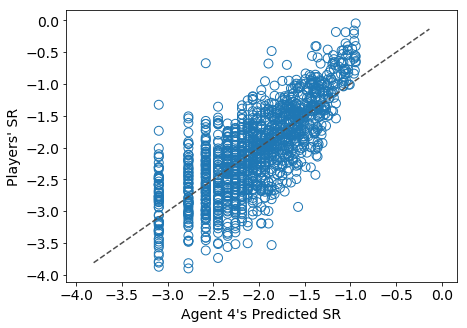
\includegraphics[width=0.31\textwidth]{masters-thesis-master/masters-thesis/contents/04_results/Player_Modeling/Clustering/plots/agent4_pred_obs.png}
    \label{fig:train_example_residuals:train_pred_obs}
    }
    \subfloat[]{%Agent 4's SR vs residuals
    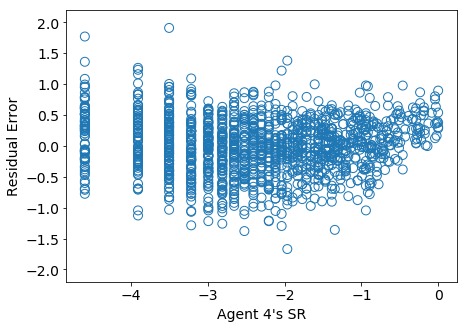
\includegraphics[width=0.31\textwidth]{masters-thesis-master/masters-thesis/contents/04_results/Player_Modeling/Clustering/plots/agent4_res_sr.png}
    \label{fig:train_example_residuals:train_sr}
    }
  \subfloat[]{%Levels vs residuals
    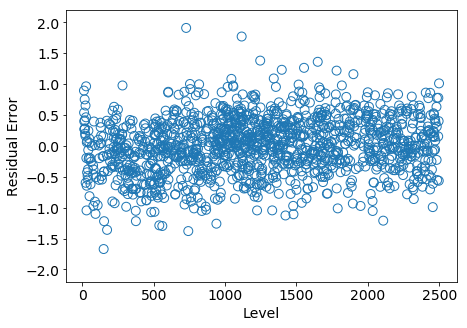
\includegraphics[width=0.31\textwidth]{masters-thesis-master/masters-thesis/contents/04_results/Player_Modeling/Clustering/plots/agent4_res_levels.png}
    \label{fig:train_example_residuals:train_levels}
    }
    
  \subfloat[]{%Residuals frequency
    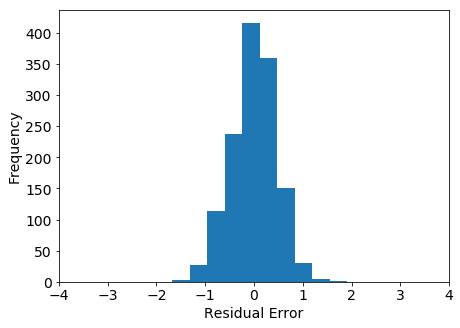
\includegraphics[width=0.31\textwidth]{masters-thesis-master/masters-thesis/contents/04_results/Player_Modeling/Clustering/plots/agent4_res_freq.png}
    \label{fig:train_example_residuals:train_frequency}
    }
  \subfloat[]{%Normal probability plot
    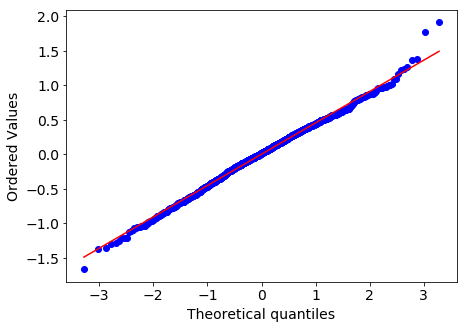
\includegraphics[width=0.315\textwidth]{masters-thesis-master/masters-thesis/contents/04_results/Player_Modeling/Clustering/plots/agent4_qq.png}
    \centering
    \label{fig:train_example_residuals:train_qq}
    }
    \caption{Plots validating the linear regression assumptions in the training data for agent 4. Figure (a) illustrates the linear relationship between the players' SR and the predicted players' SR, the black dashed line is the diagonal. Figure (b) shows the agent's SR against the residual errors while Figure (c) shows the levels against the residuals. Figure (d) shows the histogram of the residual errors and finally, Figure (e) shows the normal probability plot of the residuals.}
    \label{fig:train_example_residuals}
\end{figure}
\noindent
As an example, we check these assumptions for the linear regression model trained with agent 4's \acs{sr}. The same tests are performed with all the remaining linear models and the plots are illustrated in Appendix \ref{assamp_val}. Note, that these analysis are performed on the training data before using the linear models for prediction.
Plotting the agent 4's predicted \acs{sr} against the players' \acs{sr}, as illustrated in Figure \ref{fig:train_example_residuals:train_pred_obs}, we validated that exists a linear relationship between the dependent and the independent variables. Except for very high values of the agent's \acs{sr}, the data points are symmetrically distributed around the diagonal line. This implies that there is no major violation of the linear relationship assumption (1). 
Figure \ref{fig:train_example_residuals:train_sr} illustrates the agent's \acs{sr} against the residual errors. The variance of the errors seems to be fairly constant along the independent variable, except for very high agent's \acs{sr} where it seems to be lower. For completeness, we also checked that the variance of the errors is constant along the dependent variable and we obtained similar results. However, the residual errors seem to be centered around zero only for values of the agent's \acs{sr} between -1 and -4. For very low or very high agent's \acs{sr} the errors are not centered around zero. More precisely, when the agent's \acs{sr} is very low or very high, the residual error is more likely to be positive, meaning that we underestimate levels that are very difficult or very easy for the agent. 
% On the contrary, when the agent's \acs{sr} is high, the residual error is likely to be negative, meaning that we overestimate levels where the agent performs well.
However, since the data points that violate the homoscedasticity assumption (2) are only a small number compared to the total number of training data points, we concluded that there is only a minor violation of this assumption.
In Figure \ref{fig:train_example_residuals:train_sr}, we can also observe that consecutive errors are not correlated, therefore there is no violation of the statistical independence of the errors assumption (3). Figure \ref{fig:train_example_residuals:train_levels} shows that the errors are equally distributed along the levels as well.
Figure \ref{fig:train_example_residuals:train_frequency} illustrates the histogram of the residual errors. We can notice that the histogram seems to represent a normal distribution. Finally, we checked against violation of the normal distribution of the errors assumption (4) by looking at the normal probability plot \cite{chambers_assessing_1983} that is illustrated in Figure \ref{fig:train_example_residuals:train_qq}. We can see that only a few points at both the tails of the theoretical quantiles do not follow the line.
As a result, we can say that there is no violation of the normal distribution of the errors assumption.  

Similar conclusions can be derived for the other linear models with only few exceptions. The linear models trained with agent 1's and agent 3's \acs{sr} showed a small correlation between the levels and the residual errors. This is not surprising since the players that they simulate have a non-constant average \acs{sr} in the training data. This implies that for these two specific agents, adding the levels as a feature of the linear model could improve the performances. Moreover, the linear model trained with agent 1's \acs{sr} violates the normality of the error distribution assumption. However, this agent represent only 2\% of the total number of players and we knew that it could represents outliers or anomalous players. Since agent 1 and 3 represent only 9\% of the players in total, for practical purposes, a lower performance of the linear models for these agents is tolerable. Finally, similar plots for validating the assumptions with the baseline agent are reported in Appendix \ref{assamp_val}.
Subsequently, we use the fitted linear models to predict on test levels.
In Figure \ref{fig:test_example_residuals} we observe that the assumption we validated in the training data for the linear models still hold in the test data.
\begin{figure}[h]
  \centering
  \subfloat[]{%Players' SR against predicted SR
    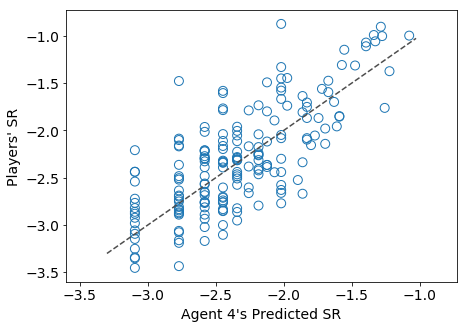
\includegraphics[width=0.45\textwidth]{masters-thesis-master/masters-thesis/contents/04_results/Player_Modeling/Clustering/plots/agent4_pred_obs_test.png}
    \label{fig:test_example_residuals:test_pred_obs}
    }
    \subfloat[]{%Agent 4's SR against residuals
    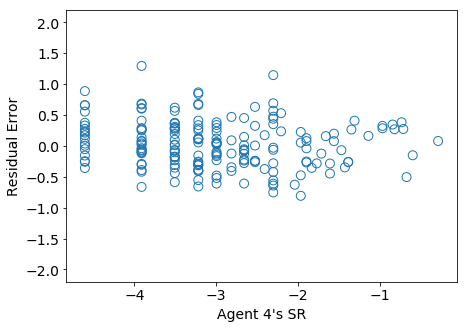
\includegraphics[width=0.45\textwidth]{masters-thesis-master/masters-thesis/contents/04_results/Player_Modeling/Clustering/plots/agent4_res_sr_test.png}
    \label{fig:test_example_residuals:test_sr}
    }
    
    \caption{Plots confirming the linear regression assumptions in the test data for the agent 4. Figure (a) illustrates the linear relationship between the players' SR and the predicted players' SR, the black dashed line is the diagonal. Figure (b) shows the agent's SR against the residual errors.}
    \label{fig:test_example_residuals}
\end{figure}
\noindent
More specifically, Figure \ref{fig:test_example_residuals:test_pred_obs} shows that there is a linear relationship between the agent's and the players' \acs{sr} in the test data while Figure \ref{fig:test_example_residuals:test_sr} shows that the residual errors are well distributed, not correlated and with a fairly constant variance.
In Figure \ref{fig:example_predictions}, as an example, we illustrate the \acs{sr} predictions of the players in cluster 4 for both the baseline and agent 4. The comparisons between the other agents and the baseline while predicting the remaining player clusters are reported in Appendix \ref{predictions_comparison}.
\begin{figure}[h]
  \centering
  \subfloat[]{%Agent 4's predictions
    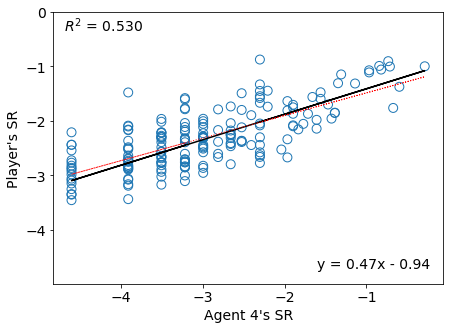
\includegraphics[width=0.45\textwidth]{masters-thesis-master/masters-thesis/contents/04_results/Player_Modeling/Clustering/plots/agent4_test_prediction.png}
    \label{fig:example_predictions:Agent 0's predictions}
    }
  \subfloat[]{%Baseline's predictions trained with all players
    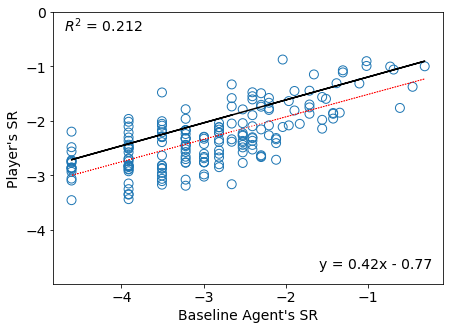
\includegraphics[width=0.45\textwidth]{masters-thesis-master/masters-thesis/contents/04_results/Player_Modeling/Clustering/plots/baseline4_test_prediction.png}
    \label{fig:example_predictions:Baseline agent's predictions}
    }
    
    \subfloat[]{%Baseline's predictions trained with players in cluster 4
    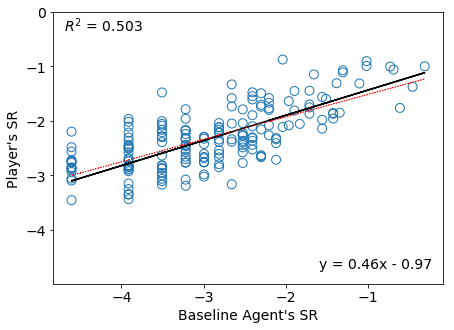
\includegraphics[width=0.45\textwidth]{masters-thesis-master/masters-thesis/contents/04_results/Player_Modeling/Clustering/plots/baseline4_test_pred_in_4.png}
    \label{fig:example_predictions:Baseline agent's predictions in 4}
    }
    \caption{Agent 4's and baseline's predictions for the success rate of players in cluster 4. Figure (a) illustrates the agent 4's predictions while Figures (b) and (c) show the predictions obtained from the baseline's SR. The baseline predictions in (b) are obtained training the baseline linear model to predict the average \acs{sr} of the players. The baseline predictions in (c) are obtained training the baseline linear model to predict the \acs{sr} of the players in cluster 4. In each graph, the black line shows the linear regression model while the red dashed line shows the ideal linear model. In the top left corner we illustrate the $R^2$ measure of the fitted regression model. In the bottom right corner of the graph we report the equation of the line obtained by the linear regression model.}
    \label{fig:example_predictions}
\end{figure}
We observe that the linear model fitted with the agent 4's \acs{sr} significantly outperforms the baseline in predicting the \acs{sr} of players in cluster 4. Moreover, we observe that the baseline approach systematically overestimates these players. This is explained by the fact that cluster 4 represents players which have a \acs{sr} distribution that is consistently under the average value. Similar reasoning can be done looking at the others agents' predictions compared to the baseline. Furthermore, Figure \ref{fig:example_predictions:Baseline agent's predictions in 4} shows that even if we train the baseline agent to predict the \acs{sr} of players in cluster 4 instead of predicting the average \acs{sr} between all the players, the prediction performances remain lower than those of agent 4. This confirms that the \acs{sr} of players in cluster 4 are more correlated to the \acs{sr} of agent 4 rather then the \acs{sr} of the baseline agent. However, if we train the baseline agent to predict the \acs{sr} of players in cluster 4 the difference with our approach in terms of \acs{sr} predictions is small. This suggest that after clustering the players, using only the baseline agent to predict each player cluster \acs{sr} could be a trade-off between computational requirements and prediction accuracy. 

Table \ref{tab:prediction_analysis} reports the MAE, MSE and adjusted R-squared computed on each player cluster. Note that on each row the "agent" columns describe a different agent, the one trained with the corresponding player cluster. For example, we never use agent 1 to predict the \acs{sr} of players in different clusters from cluster 1. On the contrary, the baseline columns indicate always the same baseline agent used to predict the \acs{sr} of players in all the defined clusters. We can observe that each linear model, compared to the baseline, better represents, in terms of \acs{sr} predictions on test levels, the players that the agent simulates. Note that the adjusted R-squared is 1 in the ideal case where the line perfectly fits all the data points but it does not have a lower bound. This means that as the linear model get worse, the adjusted R-squared value can become negative and it can decrease indefinitely.    
\begin{table}[H]
    \centering
    \small
    \caption{Analysis of the linear regression models while predicting on test data sets and comparison with the baseline agent} 
       \begin{tabular}{l c c c c S S }
    \toprule
    
    & \multicolumn{2}{c}{MAE} & \multicolumn{2}{c}{MSE} & \multicolumn{2}{c}{Adj R-squared} \\
    \cmidrule(r){2-3} 
    \cmidrule(r){4-5}
    \cmidrule(r){6-7}
    
    Players in & Agent & Baseline & Agent & Baseline & \text{Agent} & \text{Baseline} \\
    
    \midrule
    Cluster 0 & 0.27 & 0.34  &    0.12 &     0.19   &   0.47  &   0.12   \\ 
    
    Cluster 1 & 0.34 & 0.85 &    0.18 &     0.87  &   -0.27  &   -5.26  \\ 
    
    Cluster 2 & 0.33 & 0.34 &    0.16  &     0.17  &   0.34 &   0.30 \\ 
    
    Cluster 3 & 0.40 & 0.91 &    0.22 &     0.94  &   -0.99 &   -7.75 \\ 
    
    Cluster 4 & 0.31 & 0.41  &    0.15 &     0.26  &   0.49 &   0.13 \\ 
    
    Cluster 5 & 0.30  & 0.31  &    0.14 &     0.16  &   0.50 &   0.44  \\ 
    
    \bottomrule
        
    \end{tabular}
    \label{tab:prediction_analysis}
\end{table} 

A boxplot illustrating the residual errors of the agents and the baseline on each player cluster is shown in Figure \ref{fig:boxplot}. It shows that the agents have an error closer to zero and a lower variance, confirming that they can better predict the players' \acs{sr} that they represent compared to the baseline.
\begin{figure}[h!]       
    \centering
    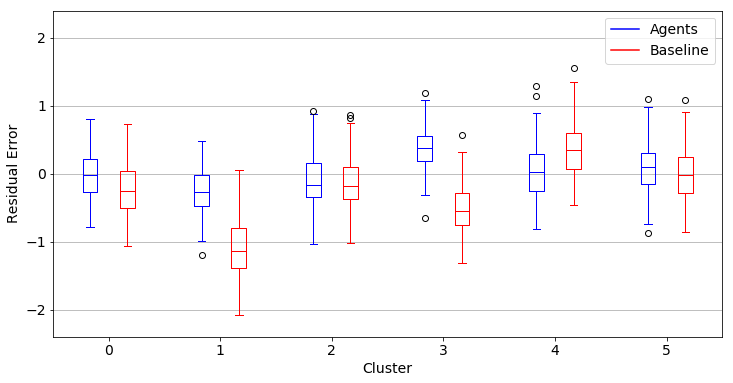
\includegraphics[width=0.6\textwidth]{masters-thesis-master/masters-thesis/contents/04_results/Player_Modeling/Clustering/plots/boxplot.png}
    \caption{Boxplot comparing agent's and baseline's residual errors. For each player cluster illustrates the distribution of the residual errors of the agent representing the cluster, in blue on the left, and the baseline approach, in red on the right.}
    \label{fig:boxplot}
\end{figure}

Finally, in order to compare our approach with the baseline approach and answer our research question we combined the agents' predictions to obtain a single measure. The linear combination of the six predictions, as defined in \ref{combination}, is based on the percentage of players that each agent represents. Table \ref{tab:prediction_performance_linear} reports the evaluation of our approach compared to the baseline. The clustering players approach reduced the prediction MAE from 0.30 to 0.26 with an improvement of 13\% and reduced the prediction MSE from 0.13 to 0.10 with an improvement of 23\%. In the table we also reported the 95\% confidence interval of the mean. We ran a paired t-test to check that the mean difference between the absolute errors per each test level is different from zero. We decided to use a paired t-test because the two approaches are tested on the same levels and we want to remove the variability in the errors that has not been completely removed by the linear regression models due to the minor violation of the homoscedasticity assumption. The paired t-test increases the statistical power of our analysis because it removes the between-level variability. If a level is too difficult, the difference between the approaches does not have to be large even if the error is big. As a result, we obtained a two-tailed p-value of 0.04\%. Since it is lower than 5\% we rejected the hypothesis of no difference between the absolute errors of the two approaches. For completeness, we ran a two-sided t-test to check that the two approaches have a statistically different \acs{MAE}. Since we obtained a p-value lower than 5\%, we can reject the null hypothesis of identical average scores. Similar results were obtained for the \acs{MSE}. As a consequence, we have strong evidence that the new approach outperforms the baseline approach. The MAE is the metric that for practical purposes we consider most important between the two. We prefer to have few wrong predictions and frequent accurate predictions rather than constantly fairly accurate predictions. This because human testing is still worth when concerning subjective or qualitative measurements like fun or player experience and if applied in conjunction with our approach, it can easily detect highly wrong predictions.
\begin{table}[h!]
    \centering
    \small
    \caption{Clustering players. Overall linear regression performance measures} 
       \begin{tabular}{l c c}
    \toprule
    
    Approach  & MAE & MSE \\ % & Adj R-squared
    
    \midrule
    Baseline            & 0.30 $\pm$ 0.03  & 0.13 $\pm$ 0.02  \\ % &   0.43 
    Clustering players  & 0.26 $\pm$ 0.03  & 0.10 $\pm$ 0.02  \\ %  &   0.56
    

    \bottomrule
        
    \end{tabular}
    
    
    %   \begin{tabular}{l c c c c}
    % \toprule
    
    % & \multicolumn{2}{c}{MAE} & \multicolumn{2}{c}{MSE} \\
    % \cmidrule(r){2-3} 
    % \cmidrule(r){4-5}
    % Approach  & Mean & Std err & Mean & Std err \\ % & Adj R-squared
    
    % \midrule
    % Baseline            & 0.30 & 0.015  & 0.13 & 0.013  \\ % &   0.43 
    % Clustering players  & 0.26 & 0.013  & 0.10 & 0.009  \\ %  &   0.56
    

    % \bottomrule
        
    % \end{tabular}
    
    
    \label{tab:prediction_performance_linear}
\end{table} 

% Furthermore, Figure \ref{fig:abs_err} illustrates the distribution of the absolute errors for the baseline and the proposed approach. We observe how with our approach the errors are more shifted toward zero compared to the baseline approach. 
% Finally, also the standard deviation of the absolute errors is reduced. The standard deviation is $0.21$ for the baseline approach and $0.18$ for the clustering players approach.
% \begin{figure}[h]
%   \centering
%   \subfloat[]{
%     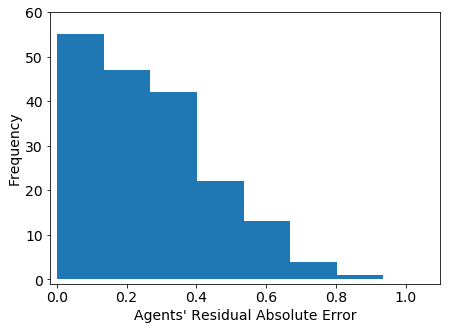
\includegraphics[width=0.45\textwidth]{masters-thesis-master/masters-thesis/contents/04_results/Player_Modeling/Clustering/plots/agents_res_abs_err.png}
%     \label{fig:example_predictions:Agents abs err}
%     }
%   \subfloat[]{
%     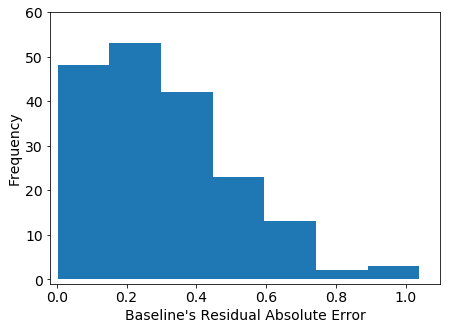
\includegraphics[width=0.45\textwidth]{masters-thesis-master/masters-thesis/contents/04_results/Player_Modeling/Clustering/plots/baseline_res_abs_err.png}
%     \label{fig:example_predictions:Baseline abs err}
%     }
    
%     \caption{Absolute error distributions. Figure (a) illustrates the distribution of the absolute errors for the clustering players approach while Figure (b) illustrates the distribution of the absolute errors for the baseline approach.}
%     \label{fig:abs_err}
% \end{figure}


\subsection*{Predictions using the mean of the players’ success rate}
Regarding data points where the agents or the baseline have a zero \acs{sr}, a prediction is formed using the mean of the players' \acs{sr} where the corresponding agent's or baseline's \acs{sr} are zero in the training data. This means that for each agent, the predictions in the test levels where the agent failed are computed by looking at the mean of the players' \acs{sr} in the training levels where the corresponding agent failed as well. In Table \ref{tab:prediction_performance_tot} we reported both the performance in the linear part and the overall prediction performance. We can say that our approach reduced the MAE by 7\% and the MSE by 4\% when considering both the linear and the mean predictions. Furthermore, we reported the 95\% confidence interval of the measurements. Note that the improvement of our approach is lower when considering the mean predictions as when considering only the linear part.
Since the agents and the baseline failed in different levels, we need to consider that the number of levels predicted with the mean is different between each agent and the baseline. On average the six agents predict 62 levels using the mean while the baseline predicts 69 levels with the mean.
We ran a paired t-test to check that the within pair difference obtained is larger than would be expected to have occurred by chance. Since we obtained a two-tailed p-value greater than 5\% we cannot reject the null hypothesis when considering also the predictions realized with the mean \acs{sr}.
\begin{table}[h]
    \centering
    \small
    \caption{Clustering players. Regression performance measures} 
       \begin{tabular}{l c c c c }
    \toprule
    
    & \multicolumn{2}{c}{MAE} & \multicolumn{2}{c}{MSE} \\
    % & \multicolumn{2}{c}{Adj R-squared}  \\
    \cmidrule(r){2-3} 
    \cmidrule(r){4-5}

    Approach & Linear part & Total & Linear part & Total  \\
    % & Linear part & Total
    \midrule
    Baseline            & 0.30 $\pm$ 0.03 & 0.31 $\pm$ 0.02 & 0.13 $\pm$ 0.02 & 0.14 $\pm$ 0.02   \\ % & 0.43 & 0.43
    Clustering players  & 0.26 $\pm$ 0.03 & 0.29 $\pm$ 0.02 & 0.10 $\pm$ 0.02 & 0.13 $\pm$ 0.02 \\  % & 0.56 & 0.46 
    
    \bottomrule
    \end{tabular}
    \label{tab:prediction_performance_tot}
\end{table} 

Figure \ref{fig:boxplot_tot} illustrates the distribution of the \acs{sr} for the failed levels of each agent as well as the mean used to predict in these cases. The players' \acs{sr} in the failed levels tend to be lower compared to the succeeded levels. This is desirable since we expect levels where the agents failed to be difficult for the players as well. However, the variance is high and as a consequence the mean prediction performs poorly. Furthermore, since the failed levels represent on average 18\% of the test levels, their impact on the regression performances is considerable. Finally, we can observe that the predicted mean in the baseline approach is closer to the true mean compared to other agents. This is due to the fact that the baseline represents a greater number of players and their average \acs{sr} is less variable between training and test levels. On the contrary, the average \acs{sr} on failed levels for some agents, especially agents 1, 2 and 3, changes a lot between training and test levels. This was expected by looking at the \acs{sr} distribution in Figure \ref{fig:k_means} and it can explain why adding these levels reduces the performances of our approach.

\begin{figure}[h!]       
    \centering
    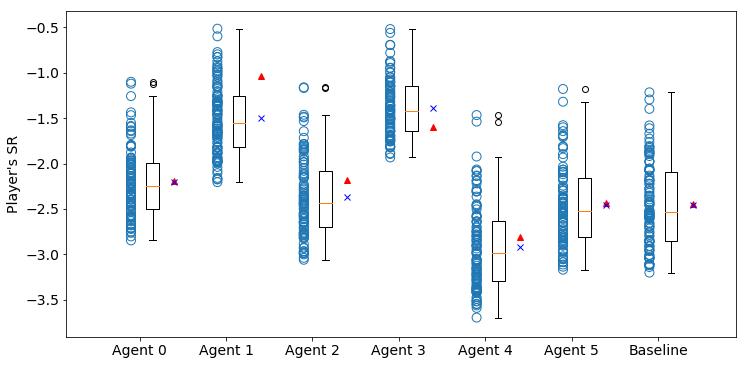
\includegraphics[width=0.6\textwidth]{masters-thesis-master/masters-thesis/contents/04_results/Player_Modeling/Clustering/plots/boxplot_zeros.png}
    \caption{Data points and boxplots of levels predicted with the mean. The red triangles show the mean prediction of each agent while the blue crosses indicated the true mean.}
     \label{fig:boxplot_tot}
\end{figure}

\subsection{Clustering Simulated Strategies Approach}

In this approach, since we cannot accurately determine how many players each agent simulates, instead of combining the predictions of six different linear models, we use a single linear regression model with six predictors.
Another difference with the previous approach is that we no longer need to eliminate levels that drastically changed since both the players' \acs{sr} and the agents' \acs{sr} are computed using the most recent and identical version of the levels.

As we did for the clustering players approach, we validated the four linear regression assumptions in the training data and we reported the plots in Appendix \ref{assamp_val_sim_strategies}. We can observe that the assumptions hold with only a minor violation of the homoscedasticity of the errors assumption. 
Subsequently, we used the linear model fitted with the six agents' \acs{sr} and the one fitted with the baseline's \acs{sr} to predict on test levels. Table \ref{tab:prediction_performance_linear_sim} reports the evaluation of our approach compared to the baseline. The clustering simulated strategies approach reduced the prediction MAE from 0.30 to 0.26 with an improvement of 13\%, the prediction MSE from 0.17 to 0.13 with an improvement of 24\% and finally improved the adjusted R-squared from 0.51 to 0.62 with an improvement of 22\%. 
We ran a paired t-test to check that the per-level mean difference of the absolute errors between the two approaches is different from zero with a significance level of 5\%. We obtained a two-tailed p-value of 0.08\% and rejected the null hypothesis concluding that the mean difference between the two approaches is statistically significantly different to zero.
For completeness, we ran a two-sided t-test to check that the two approaches have a statistically different \acs{MAE}. We obtained a two-tailed p-value lower than 5\% and we rejected the null hypothesis of identical average scores. Furthermore, since in this approach we compared a linear model with six predictors with a linear model with a single predictor, the most important metric is the adjusted R-squared because it takes into account the number of predictors. More precisely, the adjusted R-squared decreases if we add a predictor that improves the model less than what would be improved by chance.  
% Finally, also the standard deviation of the absolute errors is reduced, from $0.25$ for the baseline approach to $0.27$ for the proposed approach.
\begin{table}[h!]
    \centering
    \small
    \caption{Clustering simulated strategies. Overall linear regression performances} 
       \begin{tabular}{l c c c }
    \toprule
    
    
    Approach & MAE & MSE & Adj R-squared \\ 
    
    \midrule
    Baseline & 0.30 $\pm$ 0.04  & 0.17 $\pm$ 0.06 & 0.51  \\ 
    Clustering simulated strategies & 0.26 $\pm$ 0.03 & 0.13 $\pm$ 0.05 &  0.62 \\ 
    

    \bottomrule
        
    \end{tabular}
    
    
    
    %   \begin{tabular}{l c c c c c}
    % \toprule
    
    % & \multicolumn{2}{c}{MAE} & \multicolumn{2}{c}{MSE} & \\
    % % & \multicolumn{2}{c}{Adj R-squared}  \\
    % \cmidrule(r){2-3} 
    % \cmidrule(r){4-5}
    
    % Approach & Mean & Std err & Mean & Std err & Adj R-squared \\ 
    
    % \midrule
    % Baseline & 0.30 & 0.019 & 0.17 & 0.032 & 0.51  \\ 
    % Clustering simulated strategies & 0.26 & 0.017 & 0.13 & 0.024 &  0.62 \\ 
    

    % \bottomrule
        
    % \end{tabular}
 
    \label{tab:prediction_performance_linear_sim}
\end{table} 


\subsection*{Predictions using the mean of the players’ success rate}

The data points where any of the agents or the baseline failed are predicted using the mean of the players' \acs{sr} in the training levels where the corresponding agents or baseline failed as well.
In Table \ref{tab:prediction_performance_tot_sim} we reported the prediction performances in the linear part and the overall performances. The six agents predicted 193 levels using the mean since whenever one of the agents failed a mean prediction is applied, on the contrary, the baseline predicted only 101 levels using the mean players' \acs{sr}. Considering all predictions, the clustering simulated strategies approach achieved a 8\% lower MAE, a 16\% lower MSE and a 19\% higher adjusted R-squared than the baseline approach. However, we ran a paired t-test and we obtained a two-tailed p-value greater than 5\%. As a consequence, we cannot reject the null hypothesis of identical average scores when considering also the predictions realized with the mean \acs{sr} with a significant level of 0.05.

\begin{table}[h]
    \centering
    \small
    \caption{Clustering simulated strategies. Regression performance measures} 
       \begin{tabular}{l c c c c c c }
    \toprule
    
    & \multicolumn{2}{c}{MAE} & \multicolumn{2}{c}{MSE}  & \multicolumn{2}{c}{Adj R-squared}  \\
    \cmidrule(r){2-3} 
    \cmidrule(r){4-5}
    \cmidrule(r){6-7}

    Approach & Linear part & Total & Linear part & Total & Linear & Total \\
    \midrule
    Baseline            & 0.30 $\pm$ 0.04 & 0.35 $\pm$ 0.03 & 0.17 $\pm$ 0.06 & 0.22 $\pm$ 0.05 & 0.51 & 0.46 \\
    Clustering sim. str.  & 0.26 $\pm$ 0.03 & 0.32 $\pm$ 0.03 & 0.13 $\pm$ 0.05 & 0.18 $\pm$ 0.04 & 0.62 & 0.54 \\
    
    \bottomrule
    \end{tabular}
    
    \label{tab:prediction_performance_tot_sim}
\end{table} 

Note that the performance metrics reported in this thesis are computed on the scaled and log-transformed values. Reverting the \acs{sr} predictions and computing the errors on the original \acs{sr} values only led to different absolute values yet similar improvements between the proposed approaches and the baseline.







\chapter{Discussion}
\label{chap:discussion}

\section{Combining the Six Agents with a Single Regression Model}
In the clustering player approach, in order to have a fair comparison with the baseline that uses only a single predictor, we decided to use six linear models and combine their predictions afterwards. However, we experimented also to use a single linear model that takes as input all the six agents' \acs{sr}. We found that this model has a very similar MAE and MSE of our approach. However, looking at the p-value of each predictor we found that agent 2 has a p-value of 0.61, meaning that its predictions are not improving the model and they might be highly correlated to other agents' predictions. By removing this agent from our approach, we found that all the remaining predictors have a p-value that is lower than 5\% while the performance of the approach remained unchanged. A similar result is obtained in the clustering simulated strategies approach. The lowest p-value between the six predictors was 0.08 and removing the corresponding agent did not alter the results. This is beneficial not only for simplicity, but also for sustainability, since each time a new game content needs to be tested we have to simulate gameplay with all the developed agents. By reducing the number of simulations we will reduce the computational resources utilized. Furthermore, by providing more accurate predictions, our approaches can reduce the number of iterations required by game designers to adjust a level. However, we need to consider that the computational requirements of our approach grow linearly with the number of simulated groups of players. From the sustainability point of view, a deeper analysis of the trade-off between number of iterations and number of simulations per iteration is necessary to answer if the proposed approach is more or less sustainable than the baseline approach. Finally, since the various simulations can be executed in parallel the time required to test a game content is the same as the baseline approach.


\section{Comparison of the Two Approaches}

Even if it is not the purpose of this thesis a comparison between the two approaches may be of interest. Nevertheless, we need to remind that the agents in the two approaches are trained on different data sets and predict on different test levels.
By looking at the comparison of the two approaches with the baseline, we observe that they produce very similar improvements in the linear part. On the contrary, if we consider both the linear predictions and the mean predictions the clustering players approach only slightly improve the baseline yet being better in absolute numbers than the clustering simulated strategies approach. However, the diversity may be due to the different test levels considered in the two approaches. Note that in the clustering players approach we had to remove levels that drastically changed during time. Indeed, comparing the two approaches with the same test levels we obtained similar results.
The clustering players approach favors description and interpretation, meaning that the various agents directly simulate a specific group of players. This means that if a particular behaviour is discovered by the simulation of an agent, it is possible to go back to the players that showed this behaviour. However, it requires that meaningful player clusters are created and more importantly, that players in different clusters use, on average, different strategies. On the contrary, the clustering simulated strategy approach works better when the relationship between player features and strategies is unknown. By looking at the player features of the selected agents, it is possible to qualitatively determine which player each generated agent represents. Furthermore, during training, this approach uses all the available data and should be preferred when gameplay data are limited. However, one of the major drawback of this approach is that the feature combinations tested to select the agents grow exponentially with the number of player features. A possible solution could be to randomly select few of them or use evolutionary algorithm to explore the feature space and select the agents. In this research we aimed to model different type of players and as a consequence we selected the agents that led to more diverse strategies, however, it may be of interest to select agents based on their performance in the game or other metrics.


\section{Practical Implications}

Accurately determining the difficulty of a level is crucial for game companies since the difficulty has an impact on the revenues, both directly, in terms of boosters bought by the players and indirectly, in terms of player satisfaction and entertainment. For example, if a too difficult level is included in the game, there is a risk that frustrated players may stop playing the game. Furthermore, being able to estimate the perceived difficulty of a specific group of players, can provide an indication of how many players could be affected by a too difficult level. Additionally, it allows game designer to create levels with a desired difficulty for specific players. As an example, a game designer may want to create a level that is easy for everyone while another game designer may want to develop a level that is easier for regular players than for occasional players. 
Furthermore, it is possible to allow the \acs{CNN}-based agents to play extra moves after the maximum number of available moves is reached. Since the maximum number of moves is a parameter that game designers need to decide when creating a level, simulating longer gameplay allows to compute an estimate of how many moves to add if a level is considered too difficult for a specific type of players or globally too difficult. Furthermore, since players have the possibility to buy boosters that give them extra moves at the end of an attempt, we can estimate the potential impact of this type of boosters on different players. 

The experiments in this thesis were performed using a cloud service provider. Thanks to the fact that the training of the agents and the simulation of the gameplay can be executed in parallel, the proposed approaches scale very well with an increase of computational power. Furthermore, not only the simulation of different agents were executed in parallel, but for each agent, several copies were executed, each one simulating several attempts of the same level. As a consequence, we experimented using 1,000 attempts per level and preliminary results showed a little improvement of the players' \acs{sr} prediction.
Finally, a deeper analysis on the agents' performance discovered that for levels that contain a special item called "Sugar Key", the agents' \acs{sr} is constantly lower than the players \acs{sr}. The "Sugar Key" are key-shaped candies, which can be matched like regular candies, however they cannot be matched with any special candy. The "Sugar Key" is always present with one or more "Sugar Chest". Every time a key is destroyed, a layer of lock on the chests is removed. Removing all the chests is usually a necessary condition to complete the level. As a consequence, the lower agents' performance can be explained by the fact that a different or deeper \textit{strategic thinking} is required when this element is present on the game board, or it might be a lack of training data with these special items since they appear only on 8\% of the levels. Also the "Sugar Key" can appear in six different colors and for each color it is considered as a different input feature for the \acs{CNN}. A deeper analysis is necessary to better understand this issue.

\section{Generalization of the Results}
Despite the fact that we tested our approaches using the \textit{Candy Crush Saga} game, we believe that the same approaches, with few variations, can be applied to other games as well. Using player features to differentiate gameplay simulations and better predict players' behaviour is a general concept that can apply to many games. Furthermore, the proposed approaches could have an even bigger impact on those games where the features of the players have a stronger relationship with the player strategies \cite{holmgard_evolving_2014}. 
% For example, in a shooting game, a player that uses an handgun (player features), probably runs and shots more frequently compared to a player that uses a sniper rifle. In this case, since the relationship between player feature and actions is stronger may be captured better by the prediction model.

\textcite{drachen_guns_2012} in their research, showed how the selection of the clustering algorithm can lead to different insights of the players population. In the clustering players approach, we used k-means to extract the general distribution of players' behaviour. By using others clustering algorithms, like Simplex Volume Maximization, we could identify and model players with extremes behaviours and use them to obtain different insights about the game. Furthermore, as illustrated by \textcite{holmgard_evolving_2016}, the developed agents could be useful to characterize and classify new players by looking at which agent better represents the player decision making style.
In this thesis we focused on the players' \acs{sr} as a metric to evaluate new game content. However, the proposed approaches can be used to estimate other metrics. As an example, in \textit{Candy Crush Saga}, we can use the developed agents to estimate the score distribution and automatically set the thresholds for reaching one, two or three stars on each level. These parameters are usually set and fine-tuned by game designers.
Moreover, especially in other games, the proposed approaches could also work with completely different metrics.

Finally, the developed agents can be used for several purposes. Similarly to what \textcite{holmgard_evolving_2014} did in their research we can visualize the gameplay simulation to observe how different players interact with the game or we can use the agents to perform game balancing \cite{hunicke_case_2005}, providing each player with a slightly different level that matches their performances, skills and expectations.

\section{Limitations}
In this thesis, due to the properties of the experimented game, we used player features that are indirectly related to the player strategies. Defining, tracking and computing player features that directly relate to the performed moves, e.g. number of special candies created, could be useful to improve the developed player models. Moreover, in this work we did not consider the direction of the performed moves. Adding the possibility for the agents to chose between left-right or right-left moves and top-down or bottom-up moves can potentially increase the performances of the developed agents. Furthermore, we could also add the possibility for the agents to use in-level boosters by increasing their action space.
Another possible limitation is that the presented approaches can only be used in games where the content evolves during time since they use data from existing game content to predict on future ones. Nevertheless, in most of the \acs{F2P} games the game content is continuously added in order to engage and retain players. In addition, since we simulate gameplay using \acs{CNN}-based agents, the experimented approaches work better with games that have states that can be represented with images or encoded in a grid-shape topology, games that have a discretizable action space and games that have the Markov property. Finally, a last limitation regards the models used to predict the players' \acs{sr}. In this thesis, we used linear regression models. However, using more complex models could improve the prediction performances and a possible approach is discussed in the next section.  

\section{Future Work}

\subsection{Players' SR Prediction with Generalized Linear Models}
To overcome the limitations of the linear regression models in the players' \acs{sr} prediction stage we could try to use \acfp{GLM}. \acsp{GLM} are helpful, especially when the range of the dependent variable $y$ is restricted and the variance is not the same along the predicted values but depends on the mean of $y$. A generalized linear model is built with a linear predictor and two functions: a link function describing how the mean of $y$ depends on the predictor and a variance function describing how the variance depends on the mean. The general linear regression applied in this research is a particular case of \acs{GLM} with identity link function and unit variance. In our case, since the predicted \acs{sr} is a ratio and assumes values between 0 and 1, it could be better modeled by a binomial distribution. As a consequence a possible approach could be to use a \acs{GLM} with \textit{logit} as link function and variance function $V(\mu_i)$ defined as:
\begin{equation}
    V(\mu_i) = \mu_i(1 - \mu_i) \text{,}
\end{equation}
where $\mu_i$ is the expected value of $y$.
A preliminary experiment showed that a \acs{GLM} with binomial distribution improves the \acs{MAE} of both the proposed approaches.
Furthermore, it could be worth to model the extra uncertainty that derives from the fact that the agents play deterministically and as a consequence the agent's \acs{sr} is self-correlated. Meaning that there are some levels where the agent is always good or always bad while when we aggregate the players we average between different \acs{sr}. More work in this direction could be done to improve the performances of the proposed approaches.


\subsection{Further Applications}
The benefits of having multiple agents simulating different strategies are not limited to better estimate the players' \acs{sr} on new levels. A first extension is to compute different metrics while other applications are reported in this section and future work should deepen these aspects.

\subsubsection*{Clean the data}
 
While tracking gameplay data from players we are aware that also "noise" in the data is tracked as well. As an example, sometimes players might select moves randomly, without focusing on the game and this data are tracked as well. Having multiple agents simulating different strategies could be beneficial to reduce this noise. Our approaches help to directly model the diversity in the player strategies. However, while modeling player strategies we inevitably include the tracked "noise" in the simulated behaviour. This is especially true for casual games that can be played without too much concentration. A possible approach to discover moves that are selected randomly, is to look at the time spent by the players to select each move and compare it with the average time spent. If a move is selected very fast, this could indicate that it is just picked randomly.
Furthermore, some gameplay data are more useful to learn different player strategies than others.
If all the agents predict the same move, this means that independently from which strategy they simulate the players more likely select that specific move. Results showed that 23\% of the time all the developed agents predict the same move. It could indicate that these are states where a specific move is clearly preferred by the players. Maybe because there is only one legal move available or maybe because the predicted move leads to win the game. Since no difference is learnt from the \acsp{CNN} in these states, removing them and re-training the networks could potentially increase the differences in the simulated strategies.
Finally, we need to consider that we are simulating the strategies of groups of players and not individual ones. As a consequence it is possible that two different players, even if they belong to the same cluster, select two different moves in a given state. It is also possible that a player selects different moves even in the exact same state in two different moments. Note that in the experimented game it is hard to decide which move leads to the best outcome. By looking at the predicted probability of the \acs{CNN} we can detect the gameplay data where the network is not sure on which move is the best one. As an example we can set a threshold and if the network predicts two or more moves with probabilities that differ less than the threshold we can assume that the network is not able to decide which one is preferred and a different strategy to select the move might be appropriate in this case. In order to simulate different strategies of the same group of players we can select from the distribution of the predicted moves using different policies instead of the greedy one. This means that for example, if a move is scored $0.2$ by the \acs{CNN}, it will be selected with probability of 20\%. The \textit{softmax} function applied by the output layer guarantees that the predicted scores can be interpreted as probabilities and sum up to one. However, previous experiments showed that selecting moves in a non-greedy manner, only lead to worse performances. Future work in these directions is needed to validate or reject our hypothesis and deeper understand both the players and the game.


\subsubsection*{Categorize levels}
A possible application is to categorize levels based on the strategy required to solve them, similarly to what \textcite{isaksen_simulating_2017} have done with \textit{Tetris} and \textit{Puzzle Bubble}. The idea is to create a population of different agents each one with a different strategy level. Furthermore, the generated population can be extended by adding "strategy errors". Instead of selecting the moves with a greedy strategy, is possible to use an $\epsilon$-greedy strategy where the $\epsilon$ parameter defines how frequently each agent makes an error. The error is performed by selecting a random move instead of the one predicted by the model. Then, by comparing the performances of the agents, is possible to estimate the strategy required by each level. This approach is built on the assumption that the strategy learnt from player data is enough to solve the level. Nevertheless, we observed that on average, 82\% of the tested levels are successfully completed by the agents. 
We performed a preliminary analysis to categorize levels based on the strategy required to solve them. To obtain a meaningful analysis we restricted our focus to those levels that are successfully solved by the agent when playing with no strategy errors, using the greedy policy. We created a population of 16 different agents, each one simulating a different amount of strategy error. We randomly selected 20 levels to test this approach and we ordered the agents from the one that plays completely random (\textit{$\epsilon$ = 1}) to the one that plays greedily (\textit{$\epsilon$ = 0}). By plotting the agent's \acs{sr} against the amount of strategy used, represented by \textit{$1 - \epsilon$}, we observed how the \acs{sr} improves as we reduce the number of random moves performed. Figure \ref{fig:two_levels_strategy} shows for two levels the amount of strategy used by the agent plotted against the agents' \acs{sr}. A strategy level of zero means that the agent uses a random policy while a strategy level of one means that the agent follows a greedy policy. Note that the agents' \acs{sr} are normalized dividing them by the maximum value. This because in order to compare levels, we assume that when the agents play with full strategy they reach the optimal performances ($SR = 1$).
\begin{figure}[h]
  \centering
  \subfloat[]{%Level 154
    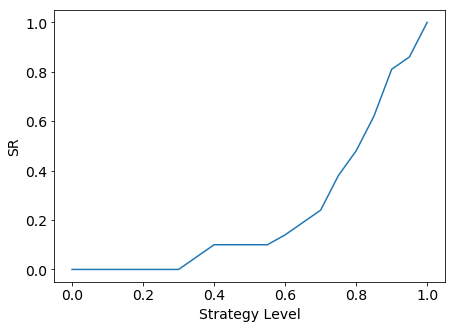
\includegraphics[width=0.45\textwidth]{masters-thesis-master/masters-thesis/contents/05_discussion/strategy_req/154.png}
    \label{fig:154}
    }
    \subfloat[]{%Level 155
    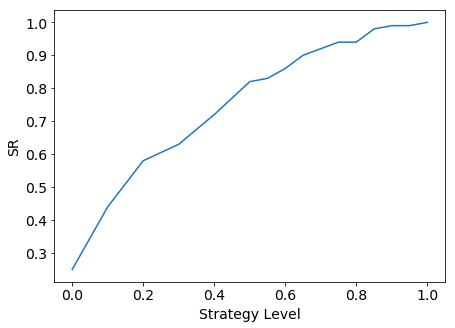
\includegraphics[width=0.45\textwidth]{masters-thesis-master/masters-thesis/contents/05_discussion/strategy_req/155.png}
    \label{fig:155}
    }
    
    \caption{Two examples of strategy requirement plots for two random levels. Figure (a) shows a level (number 154) that has a high strategy requirement while (b) shows a level (number 155) that requires less strategy to be solved. The \acs{sr} on the y-axis is normalized dividing it by the maximum value.}
    \label{fig:two_levels_strategy}
\end{figure}
To estimate the strategy required by a level we propose to use the area above the line. This metric indicates how much strategy is required to complete the levels. In the two extreme cases, the area above the line is zero when no strategy is required and the \acs{sr} is constantly equal to one independently of the amount of random moves. On the contrary, the strategy required is one when the optimal strategy is needed to solve the level and the \acs{sr} is constantly zero except for the agent that plays greedily. Having different metrics to evaluate a level can be useful for game designers to test the levels and to improve the quality of the game. Finally, we can hypothesize that levels that can be successfully solved also with random moves might be perceived less challenging by some players or that levels that require too much strategy might be an obstacle to some other players. A deeper analysis is needed to verify these hypothesis. 

In their research, \textcite{isaksen_simulating_2017} also estimated the dexterity required by each level. However the motor-skill required to correctly perform a move in \textit{Candy Crush Saga} are very low and levels that require a lot of dexterity do not exist. Nevertheless, if the proposed approaches are applied to other games it may be valuable to estimate the dexterity requirement too. Regarding \textit{Candy Crush Saga} a slightly different ability, called observability, can be modeled and estimated on each level. The idea is that players, differently from the developed agents, do not always detect all the available moves on the game board. We can add this type of error to the agents in different quantities and then estimate the observability required by each level. The error can be modeled by randomly reducing the number of available moves that the agent can select. The moves will not be selected randomly as it is for the strategy error, instead they will be selected greedily but within a subset of all the available moves. As an example, an observability of 50\% means that the agent only detects half of the available moves on each game board. As a consequence if the agent predicts a move that is not between the ones that are detected, the move is discarded and the subsequent predicted move is selected. This process is repeated until the predicted move is in the subset of the detected moves. Moreover, instead of randomly detecting the moves, different heuristics can be used to decide which moves are detected and which ones are not. As an example, we can create an agent that more often detect matches of red candies than blue candies or an agent that more often detect matches with T-shape rather than L-shape. Ideally, we could learn also these peculiarities from data.

Another application might be to classify each level based on the agreement between the agents in selecting the moves on game boards obtained from that level.
Computing the agents' agreement on several game states obtained from a specific level allows us to categorize levels based on how often different agents agree. The idea is that levels where all the agents select the same moves are less fun to play since the player strategy has a minor impact on the gameplay.
Finally, we can also categorize levels based on the predicted probabilities of the network \cite{costa_probabilistic_1996}. For example, if the network on a specific level consistently predicts a move with high probability it might indicate that the possible choices for the player are limited and as a consequence the level is less entertaining, while on the contrary if the network predicts many moves with similar probabilities it might indicate a more fun and challenging level.


% \subsection{Three Sources of Noise}
% The proposed approaches allow us to deeper understand what we call "the three source of noise" in the gameplay data. 

% First, players uses different strategies, second,  Third, even if a player is focused on selecting the best move,  Since these are properties of the players, gameplay simulation with player modeling mimics these behaviour as well. Being able to model and separate these three components might be useful to obtain better analysis. 

 
% Regarding the difficulty of evaluating the moves, we can look at the prediction accuracy of the networks. Despite the fact that we select the move with the highest accuracy, if a move is predicted with high accuracy we can say that this move is clearly perceived better than the others moves, at least from the player perspective. On the contrary, if two moves are predicted with equal probability, these could indicate that also for players is hard to evaluate which one is better.










\chapter{Conclusions}
\label{chap:conclusions}

\section{Summary}
We experimented if simulating strategies of various cohorts of players would produce agents' \acs{sr} that can be used to better predict the players' \acs{sr} on new generated game content. We proposed two different approaches to model different player strategies by directly learning them from real player data without expert knowledge. We validated our approaches using the \textit{Candy Crush Saga} game as a test bed. We tracked several player metrics and gameplay data consisting of the game board and the performed move for levels in the range [1, 2945]. In the first approach, called clustering players, we divided the tracked state-action pairs based on the performances of the players that have been tracked. Then, we trained different \acs{CNN}-based agents on each generated player cluster. On the contrary, the second approach, called clustering simulated strategies, is based on the idea of letting the network discover the relationship between player features and player strategy. We trained a \acs{CNN}-based agent that received as input three different player features in addition to the game board. Then, during prediction, by changing the input features we were able to predict different moves and as a consequence to simulate different players. We tested both of the proposed approaches against the state-of-the-art method that simulates an average strategy learnt from a random sample of real players. The goal was to understand if simulating different player strategies could generate agents' \acs{sr} that can be used to better predict players' \acs{sr} on new levels. All the simulations where performed by running 100 attempts for each level and aggregating the results to compute the agent's \acs{sr}. Then, we used linear regression models to map from the agents' \acs{sr} to the players' \acs{sr}. In the clustering players approach we fitted a different linear model for each agent and we combined the predictions based on the percentage of players that each agent simulates. In the clustering simulated strategies approach we used a single linear model that directly combines the various agents' \acs{sr}. Then, we used the developed linear models to predict players' \acs{sr} on test levels. This corresponds to how the approaches could be used in practice. The training will be done on all the available levels and the models will be used to predict on newly created levels. Finally, we compared the prediction performances of our approaches with the state-of-the-art approach. 
We found that both the approaches were able to improve the \acs{MAE} by 13\% and the \acs{MSE} by approximately 23\% in the linear regression part. Adding the mean predictions to have an estimate of the players' \acs{sr} also for levels where the agents failed reduced the improvements. However, also in this case, the proposed approaches performed better then the baseline approach. 
Furthermore, we found that not all the developed agents were strictly necessary to predict the players' \acs{sr} and reducing the number of agent maintained the same prediction accuracy while saving computational resources. We discussed how the clustering players approach favors interpretability and it can provide game designers with multiple difficulty measures, perceived by different type of players instead of only the average perceived difficulty. On the contrary, we discussed how the clustering simulated strategy approach can work without any assumption on the relationship between player features and strategies and how it allows to use all the available data during training. Finally, we discussed limitations and future work that could possibly improve the developed approaches.

\section{Conclusions}
To conclude, we have been able to model different player strategies while directly learning them from real player data. Incorporating characteristics of the players into the model allowed us to improve the prediction accuracy of the \acs{CNN}-based agents as well as the players' \acs{sr} prediction of the linear models. Furthermore, using the proposed approaches, we have been able to provide game designers with level difficulty measures perceived by different cohorts of players helping them to iteratively balance game content and create the best possible player experience.

To answer our research question, results suggested that player modeling can improve the level difficulty estimation of a \acs{CNN}-based agent simulating human gameplay. As a consequence, player modeling techniques can be used to improve automatic playtesting. In addition, the proposed approaches are general and can be extended to work with other games and different player features or to estimate different metrics. 

%------ bibliography ------x
% \emergencystretch=1.1em
\printbibliography
\cleardoublepage
\appendix
\chapter{Appendix}

\section{List of Boosters}\label{boosters}

In the following table there are all the various boosters with their description, effect, usage condition and how they look like in the game. Each row represents one booster.

\begin{table}[H]
    \caption{Full list and description of boosters}
    \centering
    \tiny
    
    \begin{tabular}{
  >{\raggedright\arraybackslash}m{.1\linewidth} % col width
  >{\centering\arraybackslash}m{.05\linewidth} % col width
  >{\arraybackslash}m{.1\linewidth} % col width
  >{\raggedright\arraybackslash}m{.1\linewidth} % col width
  >{\arraybackslash}m{.35\linewidth} % col width
}
    \toprule
    \textbf{Name} & \textbf{Image} & \textbf{Type} & \textbf{Levels} & \textbf{Effect} \\
    \midrule
    Lollipop Hammer & 
    
\includegraphics[width=0.04\textwidth]{masters-thesis-master/masters-thesis/contents/a_appendix/booster_images/Booster_lollipop_hammer.png} &
    In-level &
    All levels &
    Smash a candy (or a blockers) except chocolate spawner, ingredients, toffee tornado or sugar chest and destroy it.\\ 
    Extra Moves +5 & 
    
\includegraphics[width=0.04\textwidth]{masters-thesis-master/masters-thesis/contents/a_appendix/booster_images/Booster_extra_moves_5.png} &
    In-level, Consolation &
    All except timed levels &
    Adds five additional extra moves.\\ 
    Extra Moves +3 & 
    
\includegraphics[width=0.04\textwidth]{masters-thesis-master/masters-thesis/contents/a_appendix/booster_images/Booster_extra_moves_3.png} &
    Pre-level &
    All except timed levels &
    Adds three additional extra moves.\\
    Jelly Fish & 
    
\includegraphics[width=0.04\textwidth]{masters-thesis-master/masters-thesis/contents/a_appendix/booster_images/Booster_jelly_fish.png} &
    Pre-level &
    Jelly levels &
    Spawn 3 jelly fish at random on the gameboard.\\ 
    Colour Bomb & 
    
\includegraphics[width=0.04\textwidth]{masters-thesis-master/masters-thesis/contents/a_appendix/booster_images/Booster_color_bomb.png} &
    Pre-level &
    All levels &
    Start with one colour bomb on the gameboard.\\ 
    Coconut Wheel & 
    
\includegraphics[width=0.04\textwidth]{masters-thesis-master/masters-thesis/contents/a_appendix/booster_images/Booster_coconut_wheel.png} &
    Pre-level &
    Ingredients levels &
    Spawn a coconut wheel on the gameboard.\\ 
    Free Switch & 
    
\includegraphics[width=0.04\textwidth]{masters-thesis-master/masters-thesis/contents/a_appendix/booster_images/Booster_free_switch.png} &
    In-level &
    All levels &
    Allows the player to switch 2 candies even if they do not match.\\ 
    % Extra Time & 
    % 
\includegraphics[width=0.04\textwidth]{masters-thesis-master/masters-thesis/contents/a_appendix/booster_images/Booster_extra_time.png} &
    % Pre-level, consolation &
    % Timed levels &
    % Adds fifteen extra seconds on timed levels.\\ 
    Striped and Wrapped & 
    
\includegraphics[width=0.04\textwidth]{masters-thesis-master/masters-thesis/contents/a_appendix/booster_images/Booster_striped_and_wrapped.png} &
    Pre-level &
    All levels &
    Start the game with a wrapped and a striped candy on the gameboard.\\ 
    Sweet Teeth & 
    
\includegraphics[width=0.04\textwidth]{masters-thesis-master/masters-thesis/contents/a_appendix/booster_images/Booster_sweet_teeth.png} &
    In-level &
    All levels &
    Eats several candies, liquorice, chocolate, icing and marmalade.\\ 
    Bomb Cooler & 
    
\includegraphics[width=0.04\textwidth]{masters-thesis-master/masters-thesis/contents/a_appendix/booster_images/Booster_bomb_cooler.png} &
    In-level &
    All levels &
    Adds five extra moves to Candy Bombs. Available only if there are Candy Bombs on the gameboard.\\
    Lucky Candy & 
    
\includegraphics[width=0.04\textwidth]{masters-thesis-master/masters-thesis/contents/a_appendix/booster_images/Booster_lucky_candy.png} &
    Pre-level &
    Order levels &
    Spawn a lucky candy on the gameboard.\\ 
    Bubblegum Troll & 
    
\includegraphics[width=0.04\textwidth]{masters-thesis-master/masters-thesis/contents/a_appendix/booster_images/Booster_bubblegum_troll.png} &
    In-level &
    Levels with chocolate spawners &
    Removes all chocolate and stop the chocolate spawners for 5 moves.\\ 
    UFO & 
    
\includegraphics[width=0.04\textwidth]{masters-thesis-master/masters-thesis/contents/a_appendix/booster_images/Booster_UFO.png} &
    Pre-level &
    All levels &
    Spawn a UFO on the gameboard.\\ 
    Striped Brush & 
    
\includegraphics[width=0.04\textwidth]{masters-thesis-master/masters-thesis/contents/a_appendix/booster_images/Booster_Striped_Brush.png} &
    In-level &
    All levels &
    Allows the player to convert any regular candy into a striped candy and to choose the directions of the stripes.\\
    Party Popper & 
    
\includegraphics[width=0.04\textwidth]{masters-thesis-master/masters-thesis/contents/a_appendix/booster_images/Party_Popper_Booster.png} &
    In-level &
    All levels &
    Clears the gameboard and adds special candies.\\
    \bottomrule
    \end{tabular}

% After that, you can buy more boosters if you want to use them.
% You can also get free boosters in various ways. You can be awarded boosters by completing usually 10 levels in some games by King.com, and refill your lives. There is one booster that is only available when a Facebook or King.com friend sends you one, namely the +3 moves booster.
% As of November 27, 2013, players can obtain free boosters every day from the daily booster wheel.
% As of April 22, 2015, some players can obtain free boosters by collecting Sugar Drops on specially marked levels.
% When the player completes the final level in the Dreamworld for the first time, the player receives an award equivalent to the Jackpot.
% Some of the events will provide boosters as rewards upon completing the objective.
% In rare case if an event is glitched, there will be some boosters for making up.
% Owing to the rarity, almost all main walkthrough videos involve gameplay without boosters, and will give special notice if they are using boosters.


% Note1: Boosters shown in bold are available only in the web version, not on mobile.

% Note2: Boosters shown in strikeout are no longer available on any device.




    \label{tab:boosters}
\end{table}
    
\section{Supplement Information Regarding CNN Inputs}

In the following table there are all the input features of the \ac{CNN}. Each row represents one feature layer.

\FloatBarrier

\begin{table}[H]
    \caption{Full list of input features (1/2)}
    \centering
    \tiny
        \begin{tabular}{l l}
    \toprule
    \textbf{Layers} \\%& \textbf{Comments} \\
    \midrule
      
    REGULAR\_CANDY \\%& Encodes that the candy on that position is a regular candy\\   
    PEPPER\_CANDY \\%& Explode after a certain number of moves leading to failing the objective\\   
    MYSTERY\_CANDY \\%& Mystery candies spawn a random item when being destroyed\\   
    CHAMELEON\_CANDY \\%& A chameleon candy is a candy that changes it's color after every move\\   
    CANDY\_COLOR \\   
    CANDY\_COLOR\_RED \\   
    CANDY\_COLOR\_YELLOW \\   
    CANDY\_COLOR\_BLUE \\   
    CANDY\_COLOR\_GREEN \\   
    CANDY\_COLOR\_ORANGE \\   
    CANDY\_COLOR\_PURPLE \\   
    FISH \\  
    COCONUT\_WHEEL \\   
    INGREDIENT \\   
    EXTRA\_TIME \\ 
    MULOCK\_KEY \\   
    CHOCOLATE\_FROG \\ 
    POPCORN \\   
    UFO \\ 
    CANDY\_STRIPED\_LINE \\   
    CANDY\_STRIPED\_COLUMN \\   
    CANDY\_WRAPPED \\   
    LUCKY\_CANDY \\   

    CANDY\_CANNON\_AMMO\_CHAMELEON \\ 
    CANDY\_CANNON\_AMMO\_LUCKY \\ 
    CANDY\_CANNON\_AMMO\_TIME \\ 
    
    CONVEYOR\_BELT \\ 
    CONVEYOR\_BELT\_UP \\   
    CONVEYOR\_BELT\_RIGHT \\   
    CONVEYOR\_BELT\_DOWN \\   
    CONVEYOR\_BELT\_LEFT \\   

    CONVEYOR\_BELT\_PORTAL \\ 
    CONVEYOR\_BELT\_PORTAL\_NONE \\ 
    CONVEYOR\_BELT\_PORTAL\_RED \\   
    CONVEYOR\_BELT\_PORTAL\_BLUE \\   
    CONVEYOR\_BELT\_PORTAL\_GREEN \\   

    DIVINE\_DROP \\   
    SUGAR\_DROP \\ 
    LIGHT\_1 \\   
    LIGHT\_2 \\  
    
    LICORICE\_SQUARE \\   
    MULTI\_FROSTING\_1 \\   
    MULTI\_FROSTING\_2 \\   
    MULTI\_FROSTING\_3 \\   
    MULTI\_FROSTING\_4 \\   
    MULTI\_FROSTING\_5 \\   
    CHOCOLATE\_SPAWNER \\   
    MARMELADE\_LOCK \\   
    CANDY\_CANNON\_AMMO\_CANDY \\ 
    CANDY\_CANNON\_AMMO\_INGREDIENT \\ 
    CANDY\_CANNON\_AMMO\_LIQUORICE\_SQUARE \\ 
    CANDY\_CANNON\_AMMO\_PEPPER \\ 
    CANDY\_CANNON\_AMMO\_MULOCK\_CANDY \\ 
    CANDY\_CANNON\_AMMO\_MYSTERY\_CANDY \\ 
      
    \bottomrule
    \end{tabular}

    \label{tab:features_1}
\end{table}

\begin{table}[H]
    \caption{Full list of input features (2/2)}
    \centering
    \tiny
        \begin{tabular}{l}
    \toprule
    \textbf{Layers} \\%& \textbf{Explanation} \\
    \midrule
    
    CAKE\_BOMB \\   
    JELLY\_FROG \\ 
    MULOCK\_1 \\   
    MULOCK\_2 \\   
    MULOCK\_3 \\   
    MULOCK\_4 \\   
    MULOCK\_5 \\ 
    
    EVIL\_SPAWNER \\   
    FROGGER\_EXIT \\ 
    JELLY\_COLOR\_GREEN \\   
    JELLY\_COLOR\_RED \\   
    BOBBER \\ 
    
    VOID \\   
    EMPTY \\   
 
    CANDY\_CANNON \\ 
    STATIC\_BLOCKER \\ 
    FROSTING \\   
    LIQUORICE\_LOCK \\   
    FUDGE \\  
    INGREDIENT\_COLLECTOR \\   
    PORTAL \\ 
    PORTAL\_ENTER\_POINT \\   
    PORTAL\_EXIT\_POINT \\  
    PORTAL\_VISIBLE \\  
    PORTAL\_VISIBLE\_ENTER\_POINT \\ 
    PORTAL\_VISIBLE\_EXIT\_POINT \\  
        
      
    
    % **** Candy Orders ****
    % **** single ****
    ORDER\_CANDY\_COLOR\_RED \\ 
    ORDER\_CANDY\_COLOR\_BLUE \\ 
    ORDER\_CANDY\_COLOR\_YELLOW \\ 
    ORDER\_CANDY\_COLOR\_ORANGE \\ 
    ORDER\_CANDY\_COLOR\_PURPLE \\ 
    ORDER\_CANDY\_COLOR\_GREEN \\ 
    ORDER\_CANDY\_WRAPPED \\ 
    ORDER\_CANDY\_STRIPED \\ 
    ORDER\_CANDY\_COLOR \\ 
    ORDER\_CANDY\_FUDGE \\ 
    ORDER\_CANDY\_FROSTING \\ 
    ORDER\_CANDY\_POPCORN \\ 
    ORDER\_LIQUORICE\_SQUARE \\ 

    % **** double ****
    ORDER\_STRIPED\_STRIPED \\ 
    ORDER\_STRIPED\_WRAPPED \\ 
    ORDER\_STRIPED\_CANDY\_COLOR \\ 
    ORDER\_WRAPPED\_WRAPPED \\ 
    ORDER\_CANDY\_COLOR\_CANDY\_COLOR \\ 
    ORDER\_CANDY\_COLOR\_WRAPPED\\
    
    BIAS\_LAYER \\%& A feature plane consisting of 1.\\ 
    MOVES\_LEFT \\% & A feature plane that is 1 at every position of an candy, \\ &that can be involved in a legal move\\ 

    \bottomrule
    \end{tabular}

    \label{tab:features_2}
\end{table}






\section{Supplement Plots for the Clustering Players Approach}





\subsection{Assumption Validation on Training Levels Plots}\label{assamp_val}

\begin{figure}[H]
  \centering
  \subfloat[Agent 0]{
    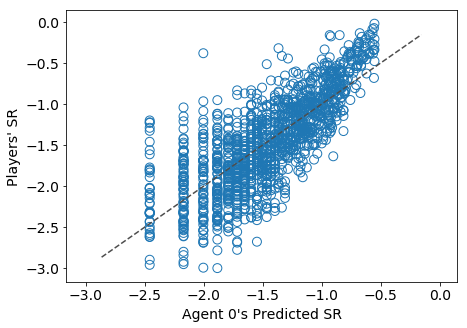
\includegraphics[width=0.31\textwidth]{masters-thesis-master/masters-thesis/contents/a_appendix/assumption_validation/pred_obs/a0.png}
    \label{fig:assamp_val:pred_obs_a0}
    }
    \subfloat[Agent 1]{
    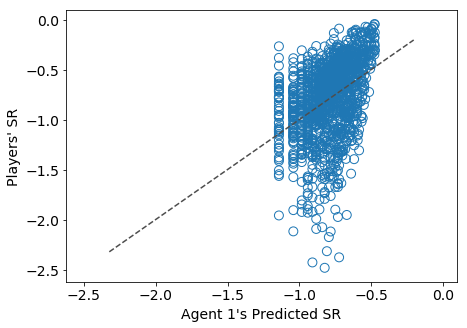
\includegraphics[width=0.31\textwidth]{masters-thesis-master/masters-thesis/contents/a_appendix/assumption_validation/pred_obs/a1.png}
    \label{fig:assamp_val:pred_obs_a1}
    }
  \subfloat[Agent 2]{
    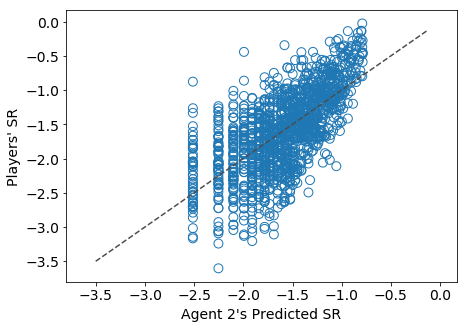
\includegraphics[width=0.31\textwidth]{masters-thesis-master/masters-thesis/contents/a_appendix/assumption_validation/pred_obs/a2.png}
    \label{fig:assamp_val:pred_obs_a2}
    }
    
  \subfloat[Agent 3]{
    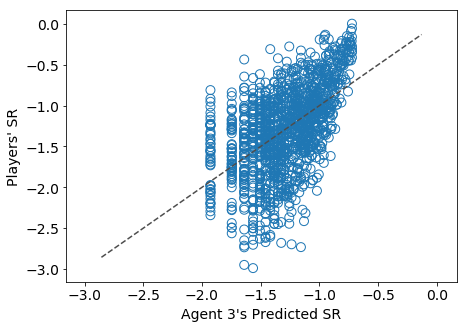
\includegraphics[width=0.31\textwidth]{masters-thesis-master/masters-thesis/contents/a_appendix/assumption_validation/pred_obs/a3.png}
    \label{fig:assamp_val:pred_obs_a3}
    }
    \subfloat[Agent 4]{
    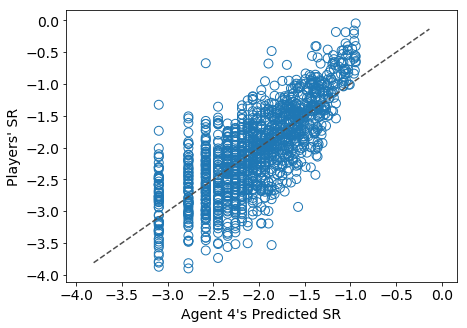
\includegraphics[width=0.31\textwidth]{masters-thesis-master/masters-thesis/contents/a_appendix/assumption_validation/pred_obs/a4.png}
    \label{fig:assamp_val:pred_obs_a4}
    }
  \subfloat[Agent 5]{
    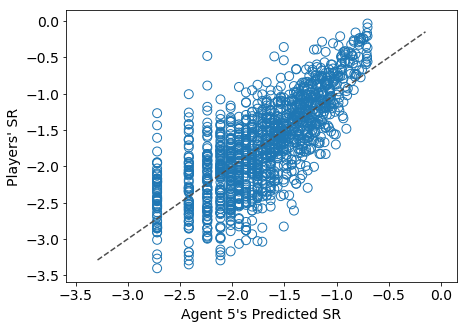
\includegraphics[width=0.31\textwidth]{masters-thesis-master/masters-thesis/contents/a_appendix/assumption_validation/pred_obs/a5.png}
    \label{fig:assamp_val:pred_obs_a5}
    }
    \caption{Players' SR against predicted SR}
    \label{fig:assamp_val:pred_obs}
\end{figure}

\begin{figure}[H]
  \centering
  \subfloat[Agent 0]{
    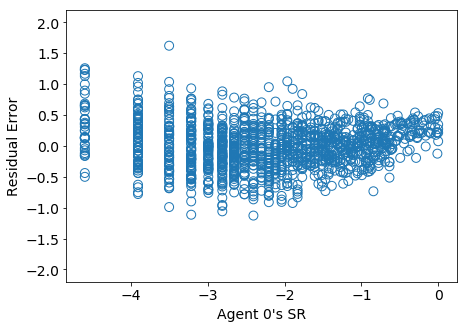
\includegraphics[width=0.31\textwidth]{masters-thesis-master/masters-thesis/contents/a_appendix/assumption_validation/res_sr/a0.png}
    \label{fig:assamp_val:res_sr_a0}
    }
    \subfloat[Agent 1]{
    \includegraphics[width=0.31\textwidth]{masters-thesis-master/masters-thesis/contents/a_appendix/assumption_validation/res_sr/a1.png}
    \label{fig:assamp_val:res_sr_a1}
    }
  \subfloat[Agent 2]{
    \includegraphics[width=0.31\textwidth]{masters-thesis-master/masters-thesis/contents/a_appendix/assumption_validation/res_sr/a2.png}
    \label{fig:assamp_val:res_sr_a2}
    }
    
  \subfloat[Agent 3]{
    \includegraphics[width=0.31\textwidth]{masters-thesis-master/masters-thesis/contents/a_appendix/assumption_validation/res_sr/a3.png}
    \label{fig:assamp_val:res_sr_a3}
    }
    \subfloat[Agent 4]{
    \includegraphics[width=0.31\textwidth]{masters-thesis-master/masters-thesis/contents/a_appendix/assumption_validation/res_sr/a4.png}
    \label{fig:assamp_val:res_sr_a4}
    }
  \subfloat[Agent 5]{
    \includegraphics[width=0.31\textwidth]{masters-thesis-master/masters-thesis/contents/a_appendix/assumption_validation/res_sr/a5.png}
    \label{fig:assamp_val:res_sr_a5}
    }
    \caption{Agent's SR against residuals}
    \label{fig:assamp_val:res_sr}
\end{figure}


\begin{figure}[h]
  \centering
  \subfloat[Agent 0]{
    \includegraphics[width=0.31\textwidth]{masters-thesis-master/masters-thesis/contents/a_appendix/assumption_validation/res_levels/a0.png}
    \label{fig:assamp_val:res_levels_a0}
    }
    \subfloat[Agent 1]{
    \includegraphics[width=0.31\textwidth]{masters-thesis-master/masters-thesis/contents/a_appendix/assumption_validation/res_levels/a1.png}
    \label{fig:assamp_val:res_levels_a1}
    }
  \subfloat[Agent 2]{
    \includegraphics[width=0.31\textwidth]{masters-thesis-master/masters-thesis/contents/a_appendix/assumption_validation/res_levels/a2.png}
    \label{fig:assamp_val:res_levels_a2}
    }
    
  \subfloat[Agent 3]{
    \includegraphics[width=0.31\textwidth]{masters-thesis-master/masters-thesis/contents/a_appendix/assumption_validation/res_levels/a3.png}
    \label{fig:assamp_val:res_levels_a3}
    }
    \subfloat[Agent 4]{
    \includegraphics[width=0.31\textwidth]{masters-thesis-master/masters-thesis/contents/a_appendix/assumption_validation/res_levels/a4.png}
    \label{fig:assamp_val:res_levels_a4}
    }
  \subfloat[Agent 5]{
    \includegraphics[width=0.31\textwidth]{masters-thesis-master/masters-thesis/contents/a_appendix/assumption_validation/res_levels/a5.png}
    \label{fig:assamp_val:res_levels_a5}
    }
    \caption{Levels against residuals}
    \label{fig:assamp_val:res_levels}
\end{figure}

\begin{figure}[H]
  \centering
  \subfloat[Agent 0]{
    \includegraphics[width=0.31\textwidth]{masters-thesis-master/masters-thesis/contents/a_appendix/assumption_validation/freq/a0.png}
    \label{fig:assamp_val:freq_a0}
    }
    \subfloat[Agent 1]{
    \includegraphics[width=0.31\textwidth]{masters-thesis-master/masters-thesis/contents/a_appendix/assumption_validation/freq/a1.png}
    \label{fig:assamp_val:freq_a1}
    }
  \subfloat[Agent 2]{
    \includegraphics[width=0.31\textwidth]{masters-thesis-master/masters-thesis/contents/a_appendix/assumption_validation/freq/a2.png}
    \label{fig:assamp_val:freq_a2}
    }
    
  \subfloat[Agent 3]{
    \includegraphics[width=0.31\textwidth]{masters-thesis-master/masters-thesis/contents/a_appendix/assumption_validation/freq/a3.png}
    \label{fig:assamp_val:freq_a3}
    }
    \subfloat[Agent 4]{
    \includegraphics[width=0.31\textwidth]{masters-thesis-master/masters-thesis/contents/a_appendix/assumption_validation/freq/a4.png}
    \label{fig:assamp_val:freq_a4}
    }
  \subfloat[Agent 5]{
    \includegraphics[width=0.31\textwidth]{masters-thesis-master/masters-thesis/contents/a_appendix/assumption_validation/freq/a5.png}
    \label{fig:assamp_val:freq_a5}
    }
    \caption{Residual frequency}
    \label{fig:assamp_val:freq}
\end{figure}

\begin{figure}[H]
  \centering
  \subfloat[Agent 0]{
    \includegraphics[width=0.31\textwidth]{masters-thesis-master/masters-thesis/contents/a_appendix/assumption_validation/qq/a0.png}
    \label{fig:assamp_val:qq_a0}
    }
    \subfloat[Agent 1]{
    \includegraphics[width=0.31\textwidth]{masters-thesis-master/masters-thesis/contents/a_appendix/assumption_validation/qq/a1.png}
    \label{fig:assamp_val:qq_a1}
    }
  \subfloat[Agent 2]{
    \includegraphics[width=0.31\textwidth]{masters-thesis-master/masters-thesis/contents/a_appendix/assumption_validation/qq/a2.png}
    \label{fig:assamp_val:qq_a2}
    }
    
  \subfloat[Agent 3]{
    \includegraphics[width=0.31\textwidth]{masters-thesis-master/masters-thesis/contents/a_appendix/assumption_validation/qq/a3.png}
    \label{fig:assamp_val:qq_a3}
    }
    \subfloat[Agent 4]{
    \includegraphics[width=0.31\textwidth]{masters-thesis-master/masters-thesis/contents/a_appendix/assumption_validation/qq/a4.png}
    \label{fig:assamp_val:qq_a4}
    }
  \subfloat[Agent 5]{
    \includegraphics[width=0.31\textwidth]{masters-thesis-master/masters-thesis/contents/a_appendix/assumption_validation/qq/a5.png}
    \label{fig:assamp_val:qq_a5}
    }
    \caption{Normal probability plots of residuals}
    \label{fig:assamp_val:qq}
\end{figure}

\begin{figure}[H]
  \centering
  \subfloat[Players' SR vs predicted SR]{
  \centering
    \includegraphics[width=0.31\textwidth]{masters-thesis-master/masters-thesis/contents/a_appendix/assumption_validation/baseline/b0.png}
    \label{fig:assamp_val:baseline_b0}
    }
    \subfloat[Baseline's SR vs residuals]{
    \centering
    \includegraphics[width=0.31\textwidth]{masters-thesis-master/masters-thesis/contents/a_appendix/assumption_validation/baseline/b1.png}
    \label{fig:assamp_val:baseline_b1}
    }
  \subfloat[Levels vs residuals]{
  \centering
    \includegraphics[width=0.31\textwidth]{masters-thesis-master/masters-thesis/contents/a_appendix/assumption_validation/baseline/b2.png}
    \label{fig:assamp_val:baseline_b2}
    }
    
  \subfloat[Residual frequency]{
  \centering
    \includegraphics[width=0.31\textwidth]{masters-thesis-master/masters-thesis/contents/a_appendix/assumption_validation/baseline/b3.png}
    \label{fig:assamp_val:baseline_b3}
    }
    \subfloat[Normal probability plot]{

    \includegraphics[width=0.315\textwidth]{masters-thesis-master/masters-thesis/contents/a_appendix/assumption_validation/baseline/b4.png}
    \centering
    \label{fig:assamp_val:baseline_b4}
    }
    \caption{Assumptions validation for the baseline}
    \label{fig:assamp_val:baseline}
\end{figure}




\subsection{Agents' and Baseline's Predictions in the Player Clusters}\label{predictions_comparison}

\begin{figure}[H]
  \centering
  \subfloat[Agent 0's predictions]{
    \includegraphics[width=0.4\textwidth]{masters-thesis-master/masters-thesis/contents/a_appendix/agents_baseline_player_clusters/a0.png}
    \label{fig:predictions_comparison:a0}
    }
    \subfloat[Baseline's predictions for cluster 0]{
    \includegraphics[width=0.4\textwidth]{masters-thesis-master/masters-thesis/contents/a_appendix/agents_baseline_player_clusters/b0.png}
    \label{fig:predictions_comparison:bo}
    }
    
  \subfloat[Agent 1's predictions]{
    \includegraphics[width=0.4\textwidth]{masters-thesis-master/masters-thesis/contents/a_appendix/agents_baseline_player_clusters/a1.png}
    \label{fig:predictions_comparison:a1}
    }
  \subfloat[Baseline's predictions for cluster 1]{
    \includegraphics[width=0.4\textwidth]{masters-thesis-master/masters-thesis/contents/a_appendix/agents_baseline_player_clusters/b1.png}
    \label{fig:predictions_comparison:b1}
    }
      
  \subfloat[Agent 2's predictions]{
    \includegraphics[width=0.4\textwidth]{masters-thesis-master/masters-thesis/contents/a_appendix/agents_baseline_player_clusters/a2.png}
    \label{fig:predictions_comparison:a2}
    }
  \subfloat[Baseline's predictions for cluster 2]{
    \includegraphics[width=0.4\textwidth]{masters-thesis-master/masters-thesis/contents/a_appendix/agents_baseline_player_clusters/b2.png}
    \label{fig:predictions_comparison:b2}
    }
    \caption{Agents' vs baseline's predictions on each player cluster (1/2)}
    \label{fig:predictions_comparison_1}
\end{figure}

\begin{figure}[H]
  \centering
  \subfloat[Agent 3's predictions]{
    \includegraphics[width=0.4\textwidth]{masters-thesis-master/masters-thesis/contents/a_appendix/agents_baseline_player_clusters/a3.png}
    \label{fig:predictions_comparison:a3}
    }
  \subfloat[Baseline's predictions for cluster 3]{
    \includegraphics[width=0.4\textwidth]{masters-thesis-master/masters-thesis/contents/a_appendix/agents_baseline_player_clusters/b3.png}
    \label{fig:predictions_comparison:b3}
    }
    
  \subfloat[Agent 4's predictions]{
    \includegraphics[width=0.4\textwidth]{masters-thesis-master/masters-thesis/contents/a_appendix/agents_baseline_player_clusters/a4.png}
    \label{fig:predictions_comparison:a4}
    }
  \subfloat[Baseline's predictions for cluster 4]{
    \includegraphics[width=0.4\textwidth]{masters-thesis-master/masters-thesis/contents/a_appendix/agents_baseline_player_clusters/b4.png}
    \label{fig:predictions_comparison:b4}
    }
    
  \subfloat[Agent 5's predictions]{
    \includegraphics[width=0.4\textwidth]{masters-thesis-master/masters-thesis/contents/a_appendix/agents_baseline_player_clusters/a5.png}
    \label{fig:predictions_comparison:a5}
    }
  \subfloat[Baseline's predictions for cluster 5]{
    \includegraphics[width=0.4\textwidth]{masters-thesis-master/masters-thesis/contents/a_appendix/agents_baseline_player_clusters/b5.png}
    \label{fig:predictions_comparison:b5}
    }
    \caption{Agents' vs baseline's predictions on each player cluster (2/2)}
    \label{fig:predictions_comparison_2}
\end{figure}



\section{Supplement Plots for the Clustering Simulated Strategies Approach}

\subsection{Assumptions Validation on Training Levels Plots}\label{assamp_val_sim_strategies}

\begin{figure}[h!]
  \centering
  \subfloat[Agents' SR vs predicted SR]{
  \centering
    \includegraphics[width=0.31\textwidth]{masters-thesis-master/masters-thesis/contents/a_appendix/assumption_validation/sim_strategies_train_agents/a0.png}
    \label{fig:assamp_val:train_agents_a0}
    }
    \subfloat[Mean agents' SR vs residuals]{
    \centering
    \includegraphics[width=0.31\textwidth]{masters-thesis-master/masters-thesis/contents/a_appendix/assumption_validation/sim_strategies_train_agents/a1.png}
    \label{fig:assamp_val:train_agentse_a1}
    }
  \subfloat[Levels vs residuals]{
  \centering
    \includegraphics[width=0.31\textwidth]{masters-thesis-master/masters-thesis/contents/a_appendix/assumption_validation/sim_strategies_train_agents/a2.png}
    \label{fig:assamp_val:train_agents_a2}
    }
    
  \subfloat[Residual frequency]{
  \centering
    \includegraphics[width=0.31\textwidth]{masters-thesis-master/masters-thesis/contents/a_appendix/assumption_validation/sim_strategies_train_agents/a3.png}
    \label{fig:assamp_val:train_agents_a3}
    }
    \subfloat[Normal probability plot]{
    \includegraphics[width=0.31\textwidth]{masters-thesis-master/masters-thesis/contents/a_appendix/assumption_validation/sim_strategies_train_agents/a4.png}
    \centering
    \label{fig:assamp_val:train_agents_a4}
    }
    \caption{Assumptions validation for the agents' linear model}
    \label{fig:assamp_val:train_agents}
\end{figure}

\begin{figure}[h]
  \centering
  \subfloat[Baseline's SR vs predicted SR]{
  \centering
    \includegraphics[width=0.31\textwidth]{masters-thesis-master/masters-thesis/contents/a_appendix/assumption_validation/sim_strategies_train_base/b0.png}
    \label{fig:assamp_val:train_base_b0}
    }
    \subfloat[Baseline's SR vs residuals]{
    \centering
    \includegraphics[width=0.31\textwidth]{masters-thesis-master/masters-thesis/contents/a_appendix/assumption_validation/sim_strategies_train_base/b1.png}
    \label{fig:assamp_val:train_base_b1}
    }
  \subfloat[Levels vs residuals]{
  \centering
    \includegraphics[width=0.31\textwidth]{masters-thesis-master/masters-thesis/contents/a_appendix/assumption_validation/sim_strategies_train_base/b2.png}
    \label{fig:assamp_val:train_base_b2}
    }
    
  \subfloat[Residual frequency]{
  \centering
    \includegraphics[width=0.31\textwidth]{masters-thesis-master/masters-thesis/contents/a_appendix/assumption_validation/sim_strategies_train_base/b3.png}
    \label{fig:assamp_val:train_base_b3}
    }
    \subfloat[Normal probability plot]{

    \includegraphics[width=0.31\textwidth]{masters-thesis-master/masters-thesis/contents/a_appendix/assumption_validation/sim_strategies_train_base/b4.png}
    \centering
    \label{fig:assamp_val:train_base_b4}
    }
    \caption{Assumptions validation for the baseline's linear model}
    \label{fig:assamp_val:train_base}
\end{figure}
\clearpage
\pagestyle{empty}
%\renewcommand*{\chapterpagestyle}{empty}
\chapter*{Declaration}




\vspace*{2cm}
\noindent
I hereby certify that I have written this thesis independently and I have only used the specified sources and resources indicated in the bibliography.

\vspace{2cm}

\noindent
Stockholm, \today

\vspace{3cm}

\hspace*{7cm}%
\dotfill\\
\hspace*{8.5cm}%
\textit{Davide Anghileri}
\clearpage

\includepdf[noautoscale,pages=2]{kth-cover}

\end{document}